\documentclass[
    iai, % Saisir le nom de l'institut rattaché
    il, % Saisir le nom de l'orientation
    %confidential, % Décommentez si le travail est confidentiel
]{heig-tb}

\usepackage[nooldvoltagedirection,european,americaninductors]{circuitikz}
\usepackage{tabularx}
\usepackage{graphicx}
\usepackage{comment}
\usepackage{pdfpages}
\usepackage{lscape}

\signature{signature_alec_berney.svg}

\setcounter{tocdepth}{1}

\makenomenclature
\makenoidxglossaries
\makeindex

\addbibresource{bibliography.bib}

\input{nomenclature}
\input{acronyms}
\newglossaryentry{heig-vd}{
    name=HEIG-VD,
    description={Haute École d'Ingénierie et de Gestion du canton de Vaud}
}
\newglossaryentry{hes-so}{
    name=HES-SO,
    description={Haute École Supérieure de Suisse Occidentale}
}
\newglossaryentry{latex}{
    name=latex,
    description={Un langage et un système de composition de documents}
}
\newglossaryentry{maths}{
    name=mathematics,
    description={Les mathematiques sont ce que les mathématiciens fonts}
}
\newglossaryentry{docker}{
    name=Docker,
    description={Docker est un outil permettant de gérer des containers, une sorte de machine virtuelle plus légère ayant pour but d'encapsuler une ou plusieurs applications / outils technologiques ainsi que toutes les dépendances que ces dernières exigent pour leur bon fonctionnement}
}
\newglossaryentry{kubernetes}{
    name=Kubernetes,
    description={Kubernetes est un système open-source permettant d'automatiser le déploiement, la mise à l'échelle et la gestion des applications conteneurisées}
}
\newglossaryentry{devops}{
    name=DevOps,
    description={Défini tout le processus conteant l'intégration continue, le déploiement continu et la livraison continue}
}
\newglossaryentry{ci}{
    name=CI,
    description={Continuous Integration / Intégration continue}
}
\newglossaryentry{cd}{
    name=CD,
    description={Continuous Deployement / Déploiement continu}
}
\newglossaryentry{github}{
    name=Github,
    description={GitHub is a website and cloud-based service that helps developers store and manage their code, as well as track and control changes to their code}
}
\newglossaryentry{gitlab}{
    name=Gitlab,
    description={GitLab is The DevOps Platform, delivered as a single application. This makes GitLab unique and creates a streamlined software workflow, unlocking your organization from the constraints of a pieced together toolchain}
}
\newglossaryentry{sgbd}{
    name=SGBD,
    description={Système de Gestion de Base de Données (DBMS), logiciel système servant à stocker, à manipuler ou gérer, et à partager des données dans une base de données}
}
\newglossaryentry{mysql}{
    name=MySQL,
    description={Système de gestion de bases de données relationnelles (SGBDR)}
}
\newglossaryentry{fablab}{
    name=Fablab,
    description={Laboratoire permettant tout type de travaux situé à la HEIG-VD }
}
\newglossaryentry{teams}{
    name=Microsoft Teams,
    description={Plateforme collaborative de visioconférence appartenant à Microsoft}
}
\newglossaryentry{backend}{
    name=Backend,
    description={Terme désignant un étage de sortie d'un logiciel devant produire un résultat. On l'oppose au front-end (aussi appelé un frontal) qui lui est la partie visible de l'iceberg}
}
\newglossaryentry{frontend}{
    name=Frontend,
    description={Partie frontale du projet affichant l'interface utilisateur permettant d'utiliser la logique du backen}
}
\newglossaryentry{bd}{
    name=BD,
    description={Une base de données permet de stocker et de retrouver des données structurées, semi-structurées ou des données brutes ou de l'information, souvent en rapport avec un thème ou une activité. Celles-ci peuvent être de natures différentes et plus ou moins reliées entre elles}
}
\newglossaryentry{rest}{
    name=REST,
    description={REST (representational state transfer) est un style d'architecture logicielle définissant un ensemble de contraintes à utiliser pour créer des services web}
}
\newglossaryentry{api}{
    name=API,
    description={Une interface de programmation d’applications ou interface de programmation applicative (souvent désignée par le terme API pour Application Programming Interface) est un ensemble normalisé de classes, de méthodes, de fonctions et de constantes qui sert de façade par laquelle un logiciel offre des services à d'autres logiciels}
}
\newglossaryentry{framework}{
    name=Framework,
    description={En programmation informatique, un framework est un ensemble cohérent de composants logiciels structurels qui sert à créer les fondations ainsi que les grandes lignes de tout ou partie d'un logiciel, c'est-à-dire une architecture}
}
\newglossaryentry{php}{
    name=PHP,
    description={Language de programmation web}
}
\newglossaryentry{laravel}{
    name=Laravel,
    description={Framework web utilisant le language de programmation php}
}
\newglossaryentry{template}{
    name=Template,
    description={Modèle de projet web frontend définissant déjà toute l'interface graphique et étant adaptable au besoin}
}
\newglossaryentry{javascript}{
    name=JavaScript,
    description={Language de programmation web}
}
\newglossaryentry{vuejs}{
    name=Vue.js,
    description={Framework web frontend utilisant le language de programmation Javascript}
}
\newglossaryentry{nodejs}{
    name=Node.js,
    description={Environnement d’exécution JavaScript construit sur le moteur JavaScript V8}
}
\newglossaryentry{ide}{
    name=IDE,
    description={Un environnement de développement est un ensemble d'outils qui permet d'augmenter la productivité des programmeurs qui développent des logiciels}
}
\newglossaryentry{os}{
    name=OS,
    description={En informatique, un système d'exploitation (souvent appelé OS — de l'anglais Operating System) est un ensemble de programmes qui dirige l'utilisation des ressources d'un ordinateur par des logiciels applicatifs}
}
\newglossaryentry{conteneur}{
    name=conteneur,
    description={Un conteneur est une sorte de machine virtuelle allégée contenant une application}
}

\newglossaryentry{tcp}{
    name=TCP,
    description={Transmission Control Protocol, abrégé TCP, est un protocole de transport fiable, en mode connecté, documenté dans la RFC 7931 de l’IETF}
}
% Auteur du document (étudiant-e) en projet de Bachelor
\author{Alec Berney}

% Activer l'option pour l'accord du féminin dans le texte
\genre{male}

% Titre de votre travail de Bachelor
\title{Gestionnaire de travaux du FabLab}

% Le sous titre est optionnel
\subtitle{Travail de Bachelor}

% Nom du professeur responsable
\teacher {Prof. Y. Chevallier (HEIG-VD)}

% Mettre à jour avec la date de rendu du travail
\date{\today}

% Numéro de TB
\thesis{7212}



\surroundwithmdframed{minted}

%% Début du document
\begin{document}
\selectlanguage{french}
\maketitle
\frontmatter
\clearemptydoublepage

%% Requis par les dispositions générales des travaux de Bachelor
\preamble
\authentification

%% Résumé / Version abbrégée
\begin{abstract}
    % Francais
Le Fablab est un laboratoire de la Haute école d'ingénierie et de gestion du canton de Vaud.
Les étudiants peuvent y réaliser toutes sortes de travaux à l'aide de machines ou outils spécifiques. Généralement, ces travaux sont demandés par les étudiants auprès de techniciens.
La gestion de ces demandes ne convient pas aux responsables du Fablab. C'est pourquoi une plateforme web dédiée à la gestion de ces demandes a déjà fait l'objet d'un précédent travail de Bachelor.
Cependant, l'application n'est pas complètement terminée et déployé. C'est pourquoi un nouveau travail de Bachelor a été proposé afin d'améliorer et de compléter ce travail.\\
La plateforme web finale permettra une meilleure gestion des échanges et commandes.\\
Cela aménera également une nouvelle dimension au niveau du suivi et de l'administration du laboratoire.\\
Une procédure claire, allant de la demande à la réalisation du travail demandé, sera également mise en place grâce à cette application.\\
Pour faciliter le suivi des demandes client, la plateforme mettra en place un système de notifications par email et sur l'application elle-même.\\
L'outil web étant à destination des utilisateurs de l'école, l'authentification via un compte de l'école sera fournie.\\

\asterism

% English
The Fablab is a laboratory of the High School of Engineering and Management of the canton of Vaud.
Here, students can carry out all kinds of work with the help of machines, devices or tools that are made available to them. Generally, these works are requested by the students to some technicians.
The management of these requests does not suit the Fablab managers.
This is why a web platform dedicated to the management of these requests has already been the subject of a previous Bachelor work. However, the application is not fully completed and deployed. Therefore, this Bachelor work has been proposed to improve and complete the work. \\
The final web platform allows a better management of exchanges and orders.
It also brings a new dimension to the follow-up and administration of the laboratory.
A clear procedure, from the request to the completion of the work, will also be put in place into this application. \\
To facilitate the follow-up of the customers' requests, the platform implements a notification system by email and on the application itself. \\
As the web tool is intended to reach school users, an authentication with school account will be provided.
\end{abstract}

%% Sommaire et tables
\clearemptydoublepage
{
    \tableofcontents
    \let\cleardoublepage\clearpage
    \listoffigures
    \let\cleardoublepage\clearpage
    \listoftables
    \let\cleardoublepage\clearpage
    \listoflistings
}

\printnomenclature
\clearemptydoublepage
\pagenumbering{arabic}

%% Contenu
\mainmatter

\chapter{Introduction}

\section{Contexte}
Le \Gls{fablab} est un laboratoire permettant de réaliser des travaux sur des machines spécifiques à ce dernier. Actuellement, pour réaliser un travail sur une machine, il est nécessaire de réaliser une demande par email à l'un des techniciens ayant le droit d'usiner sur la machine souhaitée. Une fois la demande reçue, le technicien usine dès qu'il le peut et doit recontacter le mandataire pour lui donner son travail fini. Durant toute cette période, aucun retour n'a été donné au mandataire. En cas de problème avec un travail, le technicien doit également recontacter le client.\\
Certains défauts majeurs peuvent être identifier avec la procédure actuelle, les voici :
\begin{itemize}
    \item il n'y a aucun suivi des travaux pour le mandataire, \cite{lieberherr};
    \item les échanges liés aux travaux peuvent être réalisé via plusieurs canaux (email, \Gls{teams}, vocal, etc.), \cite{lieberherr};
    \item risque de désorganisation, \cite{lieberherr};
    \item manque de clarté quant à la procédure, \cite{lieberherr};
    \item aucun historique des travaux réalisé;
    \item gestion des problèmes survenus lors du travail compliqué.
\end{itemize}
Une première partie du projet a déjà été réalisée lors du travail de Bachelor de monsieur Tristan Lieberherr. De ce fait aucun cahier des charges n'était défini à l'origine, car il était d'abord nécessaire d'effectuer une analyse du projet afin de définir les points d'améliorations qu'allaient contenir le cahier des charges.

\section{But du travail de Bachelor}
Le but, plus global, de ce travail de Bachelor, est de fournir une application web au \Gls{fablab} afin de faciliter la gestion et le suivi des demandes de travaux pour leur laboratoire.

Le but au niveau technique est de fournir une application déployée en production.\\
Il est également important de significativement améliorer le travail déjà existant en ajoutant certaines fonctionnalités et améliorant la qualité du code.\\
Cette application devra reposer sur une base de données bien conçues et ayant déjà prévu certains améliorations possibles. Elle devra également posséder un \Gls{backend} propre permettant de reprendre et l'améliorer sans devoir tout repenser.\\
La qualité de l'environnement de travail et de production ne seront pas à négliger et devront être facilement repris en main par la futur équipe s'occupant du projet.

\section{État de la situation}
Cette section permet de définir ce qui a déjà été réalisé et de l'analyser.\\
Pour commencer, il faut savoir que le travail fourni est déjà fonctionnel et fait l'objet d'une documentation suffisante pour le reprendre en main.\\
Les choix technologiques déjà réalisés et utilisés sera abordé plus tard dans le document.

\subsection{Analyse du système existant}
Dans cette partie, nous allons énumérer tous les aspects de l'ancien travail fourni. Nous n'allons
pas toucher le détail, car le but est seulement de faire ressortir les points essentiels.

\subsubsection{Environement de développement}
Pour commencer, parlons de l'environnement de travail. Il faut savoir que le projet a été transmi avec deux dépôts \Gls{github} au nom de l'ancien Bachelier et le rapport de l'ancien travail de Bachelor.

Maintenant, voici les points qui ressortent de l'analyse concernant l'environnement de travail:
\begin{itemize}
    \item deux dépôts (\Gls{repository}) \Gls{github} à son nom sont fournis;
    \item les deux dépôts ne contiennent que très peu d'information concernant le projet;
    \item le projet tourne sur d'anciennes technologies améliorées depuis;
    \item le projet n'est pas si aisément reprenable en main suite au manque d'informations concernant les technologies;
    \item l'environnement de développement est difficilement transmissible à une tierce personne, il est compliqué de vite intégrer l'équipe de développement,
    \item aucun outil de collaboration n'est fourni, nous parlons ici de \Gls{devops} (\Gls{ci} et \Gls{cd}).
\end{itemize}

\subsubsection{Base de données}
Cette partie défini tout ce qui touche à la base de données et influence également le \Gls{backend}.\\
Les points ressortant de l'analyse de la base données sont les suivants:
\begin{itemize}
    \item la base de données contient les ressources principales (utilisateurs, travaux, messages, fichiers);
    \item la base de données possèdent de la redondance paraîssant inutile;
    \item la base de données ne peut pas intégrer la gestion de plusieurs rôles;
    \item la base de données n'intégrent pas la notion de machines et de catégories de travaux;
    \item la gestion des types de fichiers acceptés pour les travaux n'est pas présente.
\end{itemize}

\newpage

\subsubsection{Backend / API}
Passons maintenant au \Gls{backend} qui est la plus grosse partie du travail.\\
Il faut savoir que toute l'analyse de la base de données s'applique également pour une bonne partie du \Gls{backend} et ne sera pas répétée.\\
Les points ressortant de l'analyse de ce dernier sont les suivants:
\begin{itemize}
    \item le principe \Gls{rest} n'est pas respecté en ce qui concerne l'\Gls{api};
    \item les entrées utilisateurs ne font l'objet d'aucune vérification syntaxique et sémantique;
    \item l'architecture de code ne respecte pas totalement celle mise à disposition par \Gls{laravel};
    \item le code n'utilise pas toutes les possibilités utiles fournies par le \Gls{framework};
    \item le contrôle de l'accès aux ressources via des rôles n'est pas mis en place;
    \item le système de stockage de fichier est fonctionnel;
    \item le système de notification est fonctionnel, mais non sécurisé;
    \item les travaux d'arrière plan envoyant des emails est fonctionnel;
    \item le Backend utilise une version antérieur du \Gls{framework};
    \item le Backend est actuellement entièrement fonctionnel.
\end{itemize}

\subsubsection{Frontend}
Finalement, passons au \Gls{frontend}, ce dernier a été réalisé à l'aide d'un \Gls{template}. Il a été adapté aux besoins de l'application. Le but du projet n'étant pas concentrer sur le \Gls{frontend}, seul une analyse de surface a été réalisée.\\
Les points ressortant de l'analyse de ce dernier sont les suivants:
\begin{itemize}
    \item le \Gls{frontend} est fonctionnel;
    \item le projet possède des dépendances obsolètes et non mise à jour;
    \item les valeurs textuelles sont toutes insérées directement dans le code et n'offre pas la possibilité de traduire facilement le site;
    \item les valeurs concernant les machines et les catégories de travaux sont \emph{hardcodées} dans le \Gls{frontend}.
\end{itemize}

\subsection{Propositions d'améliorations}

\subsubsection{Environement de développement}
Concernant l'environnement de travail, il est important d'améliorer significativement la façon dont
une personne peut s'intégrer au travail, à l'équipe de développement.\\
Pour commencer, il est nécessaire de créer une orgranisation \Gls{github} accueillant les 2 dépôts Github.
Chaque dépôt devra lister les technologies utilisées et indiquer comment les installer, ainsi que
comment configurer facilement son environnement de travail afin de participer au projet.\\
Il sera également nécessaire de réaliser un suivi du travail grâce aux outils fourni par \Gls{github} (issues, kanban, milestones, etc.).\\
Fournir un environement aisément configurable pour tout un chacun est également un point essentiel.
Une \Gls{ci} devra impérativement être mise en place afin de faciliter le travail à plusieurs sur le projet. Il en va de même pour le CD, si l'on souhaite déployer aisément les différentes versions de l'application.

\newpage

\subsubsection{Base de données}
La base de données fera l'objet d'une toute nouvelle conception pour améliorer tous les points énumérés précédement et intégrer les notions manquantes. Le Backend en sera fortement influencé.

\subsubsection{Backend}
Le \Gls{backend} étant fortement influencé par la base de données, ce dernier se verra adminsitrer de gros changements.\\
Les sujets sur lequel une amélioration devra être apportée sont les suivants:
\begin{itemize}
    \item le principe \Gls{rest} devra être appliqué;
    \item les entrées utilisateurs devront au moins faire l'objet d'une vérification syntaxique et peut-être sémantique;
    \item l'architecture de code se rapprochera le plus possible de ce qui est proposé par Laravel;
    \item le code utilisera le plus possible les outils fournis par le \Gls{framework};
    \item le contrôle de l'accès aux ressources via des rôles sera mis en place;
    \item le système de notification pourra être sécurisé et fera appel à l'\Gls{api};
    \item le \Gls{backend} passera à la nouvelle version du \Gls{framework}.
\end{itemize}

Après avoir lister tous ces points, on se rend compte que le \Gls{backend} devra presque être réaliser de
zéro. Ce ne sera pas totalement le cas, car, sur certains points, l'ancien projet sera toujours
présent comme référence en cas de questions ou de doutes.

\subsubsection{Frontend}
Les améliorations possibles concernant le \Gls{frontend} gravite essentiellement autour de la mise à jour des dépendances du projet et la façon dans les valeurs sont stockées.\\
Un système de gestion des langues (ii8n) pourrait être envisagé, ainsi que vérifier les entrées utilisateurs.\\
Le \Gls{frontend} sera surtout modifié pour être adapté aux changements du \Gls{backend}.

\section{Cahier des Charges}

\subsection{Prologue}

Le projet étant déjà existant, aucun cahier des charges n'était défini à l'origine. En effet, il était d'abord nécessaire de réaliser une analyse du projet afin de définir les points d'améliorations qu'allaient contenir le cahier des charges.

\subsection{Objectifs \label{objectifs}}

Les objectifs principaux du projet sont les suivants:
\begin{itemize}
    \item mettre en place une infrastructure de développement professionnel;
    \item mettre en place les \Gls{devops} pour le projet existant;
    \item améliorer la conception de la base de données en ajoutant des données précieuses;
    \item améliorer le \Gls{backend} du projet existant.
\end{itemize}

\newpage
Nous allons maintenant passer à la liste des tâches qui devront être effectuées durant le travail de Bachelor.

Pour les toutes les tâches qui seront listées plus bas, celles qui nécessitent une décomposition en plusieurs tâches voient le numéro de ses sous-tâches suivi d'une lettre. Les tâches possédant des sous-tâches des priorités différentes, n'auront aucune priorité globale.

Je m'engage à réaliser les tâches énumérées dans le tableau \ref{taches}.

\begin{table}[h]
    \begin{center}
        \caption{Liste des tâches / exigences à réaliser durant le projet \label{taches}}
        \begin{tabularx}{1.0\textwidth} {l|X|r}
            No. & Tâche / Exigence                                                                                                       & Priorité      \\ \hline
            1   & Créer une infrastructure de développement professionnel                                                                & Obligatoire   \\
            2   & Mettre en place un \emph{pipeline} DevOps complet                                                                      & Obligatoire   \\
            2.a & Mettre en place la CI                                                                                                  & Obligatoire   \\
            2.b & Mettre en place la CD                                                                                                  & Obligatoire   \\
            2.c & Mettre en place une infrastructure de production accueillant le rendu du projet                                        & Obligatoire   \\
            3   & Mettre à jour le projet existant vers les nouvelles versions des technologies utilisées                                & Obligatoire   \\
            3.a & Mettre à jour le frontend                                                                                              & Obligatoire   \\
            3.b & Mettre à jour le backend                                                                                               & Obligatoire   \\
            4   & Reconcevoir la base de données                                                                                         & Obligatoire   \\
            4.a & La base de données doit prendre en compte les rôles des utilisateurs                                                   & Obligatoire   \\
            4.b & La base de données doit prendre en compte les ressources liées aux machines industrielles utilisées dans l'application & Obligatoire   \\
            5   & Améliorer le backend du projet                                                                                         &               \\
            5.a & Appliquer les standards de programmation web (REST)                                                                    & Obligatoire   \\
            5.b & Mettre en place une architecture de code cohérente                                                                     & Obligatoire   \\
            5.c & Mettre en place une vérification des entrées utilisateurs                                                              & Obligatoire   \\
            5.d & Mettre en place l'authentification de l'utilisateur                                                                    & Obligatoire   \\
            5.e & Ajouter la gestion des rôles des utilisateurs                                                                          & Obligatoire   \\
            5.f & Ajouter la gestion des ressources liées aux machines industrielles utilisées dans l'application                        & Intermédiaire \\
            5.g & Améliorer le système de notifications pour le rendre plus sécurisé                                                     & Basse         \\
            6   & Améliorer le Frontend                                                                                                  &               \\
            6.a & Mettre à jour le Frontend pour coller aux modifications des routes du backend / de l'api                               & Obligatoire   \\
            6.b & Ajouter la gestion des ressources liées aux machines industrielles utilisées dans l'application                        & Intermédiaire \\
            6.c & Améliorer le système de notifications pour le rendre plus sécurisé                                                     & Basse         \\
            7   & Tester l'application à l'aide de tests automatisés                                                                     & Obligatoire   \\
            7.a & Réaliser des tests unitaires automatisés                                                                               & Obligatoire   \\
            7.b & Réaliser des tests d'intégration automatisés                                                                           & Obligatoire   \\
        \end{tabularx}
    \end{center}
\end{table}

\newpage
\subsection{Déroulement global projet}

Le projet se réalise durant le semestre de printemps. Le semestre possède 14 semaines de travail de 1 jour et demi de travail si nous excluons la semaine du CRUNCH et celle des vacances.\\
Il y a ensuite 6 semaines à temps plein pour finaliser le travail de Bachelor.

Une séance hebdomadaire est prévue avec le professeur responsable du travail, m. Chevallier.

Le projet est réparti en 3 principales phases, qui s'effectueront dans l'ordre suivant:
\begin{enumerate}
    \def\labelenumi{\arabic{enumi}.}
    \item L'analyse du projet:
          \begin{enumerate}
              \def\labelenumii{\alph{enumii}.}
              \item L'étude du projet et de ses technologies,
              \item Les choix technologiques et conceptuels.
          \end{enumerate}
    \item La conception et réalisation du projet, contenant principalement:
          \begin{enumerate}
              \def\labelenumii{\alph{enumii}.}
              \item La mise en place des environnements de développement et de production,
              \item La réalisation des \Gls{devops},
              \item L'amélioration du \Gls{backend} et de la base de données,
              \item La modification du \Gls{frontend}.
          \end{enumerate}
    \item La préparation des livrables.
\end{enumerate}

La première phase d'analyse a pour objectif de définir tout le cadre théorique du projet et les divers choix à réaliser tout au long de ce dernier.\\
Cette phase devrait se terminer à la fin de la semaine numéro 7 ou 8.\\
Tout en sachant que cette phase contient l'écriture du cahier des charges et que ce dernier doit être rendu au plus tard 6 semaines après le début du travail de bachelor, c'est-à-dire, le 10.04.2022.

La seconde phase, concernant la conception et la réalisation du projet est la plus conséquente.
Cette dernière suivra la première et devrait se terminer lors de la 20ème semaine si tout se déroule comme prévu.

La dernière phase, concernant la préparation des livrables, est une phase importante qui se réalisera tout au long du projet et se terminera la dernière semaine du travail de bachelor.

Un rendu intermédiaire est également prévu après 150 heures de travail et possède comme date le 11.05.2022.

\subsection{Résultats attendus}

Les résultats attendus pour ce projet dépendent énormément des tâches établies définies dans la partie \ref{objectifs} du cahier des charges.\\
En effet, chaque tâche définie est vérifiable et sera donc utilisée pour évaluer le résultat du projet.
\newpage

% cliffhanger

\chapter{Analyse}

\section{Choix technologiques}

Dans cette section, je vais énumérer tous les choix technologiques ou conceptuels liés au projet.
Mais avant cela, il est nécessaire de définir précisément les besoins pour le projet afin de réaliser des choix cohérents en fonction de ces derniers.\\
Pour chaque choix, technologiques ou conceptuels, une liste des possibilités réalisables sera énumérée et si possible représentée visuellement.\\
Cette liste de possibilités sera accompagnées des avantages et inconvénients de chaque solution en s'inspirant des besoins du projet.

\subsection{Rappel des choix technologiques déjà effectués}
Dans cette section, je vais énumérer les choix technologiques déjà effectués par le premier étudiant ayant travaillé sur le projet.\\
Considérant les choix de l'étudiant comme bon et bien argumenté, je ne vois aucune raison de les remettre en question, surtout qu'un travail conséquent a déjà été réalisé avec les technologies choisies.

Voici un résumé des décisions prises lors de la première phase du projet:
\begin{enumerate}
    \item \Gls{backend}: \Gls{php} avec le \Gls{framework} \href{https://laravel.com/}{Laravel}.
    \item \Gls{frontend}: \Gls{javascript} avec \href{https://vuejs.org/}{Vue.js}.
    \item \Gls{sgbd}: \href{https://www.mysql.com/}{MySQL}.
    \item Outil \emph{SSO}: \href{https://www.switch.ch/aai/about/shibboleth/}{Shibboleth}.
\end{enumerate}

En résumé, monsieur Lieberherr avait principalement choisi \Gls{laravel} pour sa simplicité et la rapidité à créer un \Gls{backend} fonctionnel. \\
En ce qui concerne le \Gls{frontend}, le \Gls{framework} \Gls{vuejs} a été choisi car il était simple à prendre en main et un modèle (\Gls{template}) de site avait déjà été trouvé et correspondait au besoin de l'application. \\
En ce qui conerne la base de données, le \Gls{sgbd} \Gls{mysql} a été choisi pour sa popularité, sa facilité de prise en main et le fait qu'il soit relationnel. \\
Pour finir, l'authentification via l'outil \emph{SSO} et \emph{Shibboleth} a été presque imposé car une une authentification scholaire avec les comptes \emph{Switch} était demandée.

Pour plus de précisions sur ces choix technologiques, je vous invite à consulter son \href{https://tb.heig-vd.ch/7532}{rapport}.

Au final, la \emph{stack} de technologies que nous allons utilisés est disponible sur le tableau \ref{stack}.

\begin{table}[h]
    \begin{center}
        \caption{Stack de technologies utilisées avec versions \label{stack}}
        \begin{tabularx}{1.0\textwidth} {X|X}
            Technologie & Version         \\ \hline
            PHP         & 8.1.8           \\
            Composer    & 2.3.9           \\
            Laravel     & 9.2             \\
            Node.js     & 14.16.1         \\
            NPM         & 6.14.12         \\
            Vue.js      & 2.6.14          \\
            HTML        & 5               \\
            CSS         & 3               \\
            Ubuntu      & 20.04 LTS       \\
            Apache      & 2               \\
            MySQL       & 8.0.30 (latest) \\
            GitHub      &                 \\
            Docker      & 20.10.17        \\
        \end{tabularx}
    \end{center}
\end{table}

% cliffhanger
Les anciens choix technologiques expliqués, il est temps de passer aux besoins que nous avons pour ce projet afin de plus tard justifier les choix que nous allons réaliser.

\subsection{Besoins pour le projet}
Je vais ici définir les besoins du projet et ceci en les séparant par parties distinctes.

\subsubsection{Besoins pour l'infrastructure de développement}
Pour commencer, définissons l'infrastructure de développement.\\
L'infrastructure de développement englobe tous les outils à installer et toutes les configurations à réaliser sur un pc vierge afin que le développeur puisse commencer à développer l'application.

En général, ce qui est recherché, c'est la simplicité et la rapidité de configuration de cet environnement.

Nous allons essentiellement nous concentrer sur les outils à installer spéficiquement pour notre projet qui sont les suivants:
\begin{itemize}
    \item le \Gls{sgbd} (Système de Gestion de Base de Données);
    \item le language \Gls{php}, avec Composer et le \Gls{framework} \Gls{laravel};
    \item l'environement d'exécution (runtime environment) Node.js et le \Gls{framework} Vue.js.
\end{itemize}

Pour l'infrastructure de développement nous recherchons avant tout:
\begin{itemize}
    \item la simplicité de mise en place du projet;
    \item la facilité de prise en main du projet;
    \item la disponbilité des outils utilisés;
    \item la difficulté à mettre en place cette infrastructure.
\end{itemize}

% cliffhanger
Après avoir défini les besoins pour notre infrastructure de développement, il faut faire de même avec celle de production et c'est ce que nous allons faire.

\newpage

\subsubsection{Besoins pour l'infrastructure de production}
Pour commencer, l'infrastructure de production englobe tous les outils à installer et toutes les configurations à réaliser sur une machine de production vierge afin que le programme final soit accessible est utilisable par n'importe quel utilisateur.

En général, la simplicité de mise à jour du programme, la performance et la robustesse sont recherchées.

Pour une machine de production, il est nécessaire d'installer les mêmes outils qu'en développement.Cependant, certains outils et programmes doivent être ajouter et ce sont principalement les suivants:
\begin{itemize}
    \item un serveur \Gls{http};
    \item un \Gls{proxy}.
\end{itemize}

Les critères qui influenceront notre décision sur l'infrastructure de producton sont:
\begin{itemize}
    \item la performance de l'infrastructure;
    \item la simplicité de mise à jour du programme au sein de l'infrastructure;
    \item la robustesse de l'infrastructure;
    \item la simplicité de mise en place de l'infrastructure;
    \item la flexibilité de l'infrastructure.
\end{itemize}

% cliffhanger
Après avoir défini les besoins pour notre infrastructure de développement et de production, nous aimerions savoir ce qu'il faut pour réussir à assurer une bonne transition entre l'environnement de développement et de production. C'est pourquoi nous allons maintenant voir les besoins des \Gls{devops}.

\subsubsection{Besoins pour les Devops}
Le \emph{pipeline} \Gls{devops} défini toutes les étapes réalisées et les outils utilisé pour parvenir à mettre en place une infrastructure de travail et de livraison de produit fonctionnel et automatisée au maximum.\\
Le but des \Gls{devops} étant d'automatisé le plus de tâches possibles, on attend donc du \emph{pipeline} les critères suivants:
\begin{itemize}
    \item la performance de l'infrastructure (dans le sens de la rapidité);
    \item la simplicité de mise en place du \emph{pipeline};
    \item la simplicité de mise à jour du \emph{pipeline};
    \item la robustesse du \emph{pipeline};
    \item la possibilité d'ajouter des étapes intermédiaires de tests du produit entre l'infrastructure de développement et de prodution.
\end{itemize}

\subsubsection{Importance de l'open source et de la gratuité des outils}
Pour tous les choix technologiques qui vont être réaliser, un besoin essentiel intervient.
Plus nous utilisons d'outils open source ou gratuit, plus nous faciliterons l'intégration de n'importe quel développeur au projet.\\
Mais utiliser des outils qui sont gratuits ou open source offre également un plus pour l'intégration aux \Gls{devops} car il facilitera de façon non négligeable la mise en place de ces derniers.

% docker
Dans la suite de ce chapitre, nous allons beaucoup parler de \Gls{docker} et des autres solutions de \Gls{conteneur}, c'est pourquoi une introduction et analyse de l'outil est disponible en annexe de ce rapport.

% dev
\subsection{Infrastructures de développement}

\subsubsection{Présentation des infrastructures de développement possibles}

%\figi{infrastructure-dev-choix.drawio}{18cm}{Différentes possibilités d'infrastructure de développement}
\begin{center}
    \begin{figure}[H]
        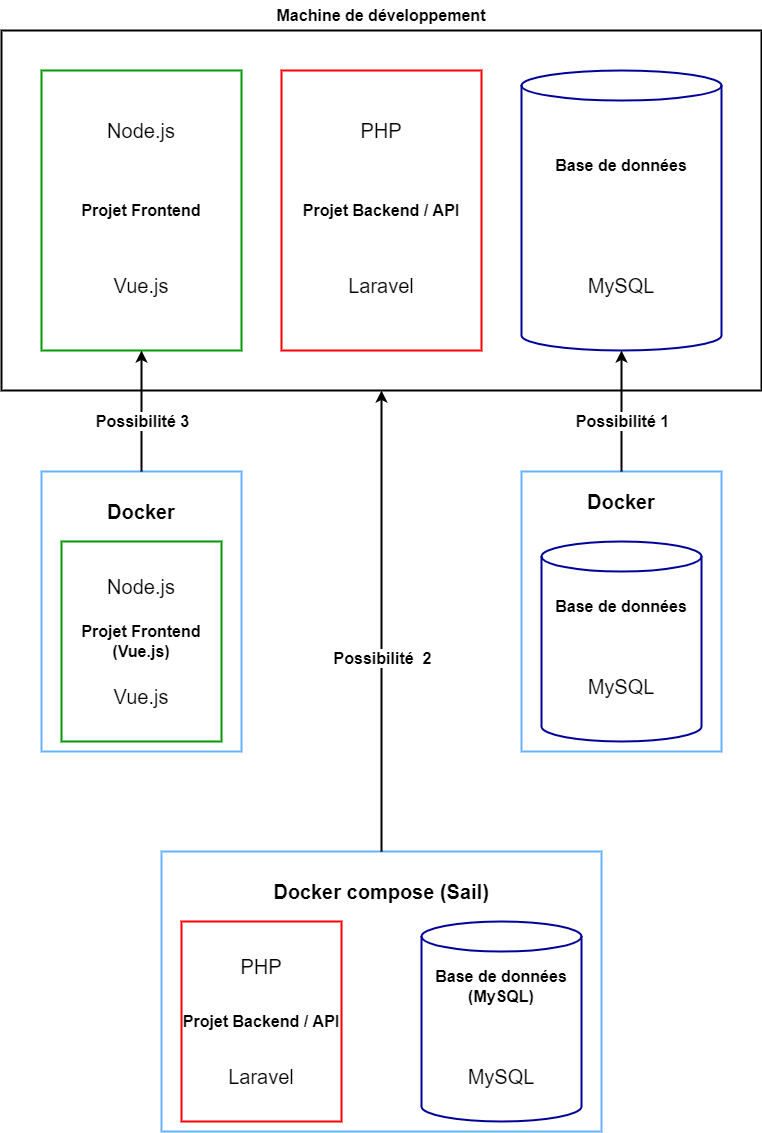
\includegraphics[width=\textwidth]{./assets/figures/infrastructure-dev-choix.drawio.png}
        \caption{Différentes possibilités d'infrastructure de développement \label{infrastructure-dev-choix.drawio}}
    \end{figure}
\end{center}

La figure \ref{infrastructure-dev-choix.drawio} représente l'infrastructure de développement actuelle avec chacune des possibilité d'amélioration. \\
On constante que tous les outils ont été installés nativement sur la machine de développement sans virtualisation ou conteneurisation.

Le premier changement pouvant être effectué est d'utiliser une infrastructure avec uniquement la base de données en \Gls{conteneur} \Gls{docker} et le reste installer nativement, comme montré avec la possibilité numéro 1.

Le second changement, est de passer tout l'environnement de développement du \Gls{backend} sous plusieurs \Gls{conteneur}s \Gls{docker} en utilisant un outil fourni par Laravel, \href{https://laravel.com/docs/9.x/sail}{Sail}. Ce changement correspond à la possibilité 2.

\Gls{laravel} proposait un outil nommé \href{https://laravel.com/docs/9.x/homestead}{Homestead} qui est un environnement de développement virtualisé à l'aide d'une machine virtuelle \href{https://www.vagrantup.com/}{Vagrant}. \\
Cette solution est considérée comme le prédecesseur à \Gls{laravel} Sail.\\
C'est pourquoi, cette solution ne fera pas parti des choix que nous allons argumenter, mais est
présentée comme complément sur la figure \ref{infrastructure-dev-laravel-homestead.drawio}.

%\figi[Infra. dev. avec Homestead]{infrastructure-dev-laravel-homestead.drawio}{16cm}{Infrastructure de développement avec Laravel Homestead}

\begin{center}
    \begin{figure}[H]
        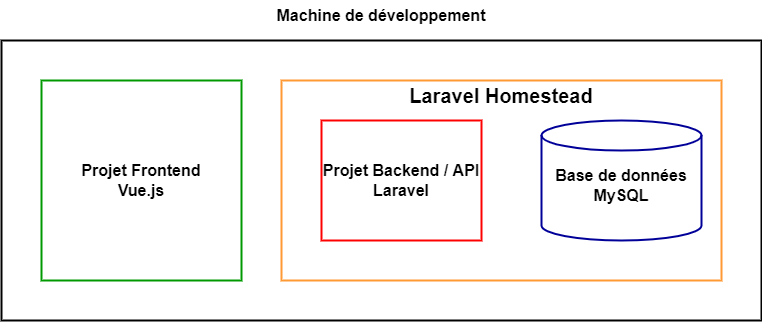
\includegraphics[width=\textwidth]{./assets/figures/infrastructure-dev-laravel-homestead.drawio.png}
        \caption{Infrastructure de développement avec Laravel Homestead \label{infrastructure-dev-laravel-homestead.drawio}}
    \end{figure}
\end{center}

Finalement, le dernier changement serait de créer un \Gls{conteneur} \Gls{docker} pour le projet \Gls{vuejs}. Ce changement correspond à la possibilité 3.

%https://laravel.com/docs/9.x/sail
%https://blog.logrocket.com/laravel-and-docker-a-guide-to-using-laravel-sail/
%https://r00t4bl3.com/post/how-to-setup-docker-environment-for-laravel-development
%https://dockerize.io/guides/php-laravel-guide
%https://www.honeybadger.io/blog/laravel-docker-php/

\clearpage

% vraiment bien se blinder au niveau des arguments via blog et études, sources écrites
% si on a pas trouvé, on peut dire je ne sais pas, on DOIT dire -> joker ultime
% toucher quelque chose en surface, si je ne connais pas, si point essentiel dans projet, faire un choix + essai -> prototype, démonstration sur expérience
% aussi parlé des charges qui devront être supportées et si c'est possible, nb user final par ex

\subsubsection{Évolutions de l'infrastructure de développement possibles}
Les différentes infrastructures désormais présentées, il est nécessaire de les comparer en listant les pours et les contres de chaque changement en prenant comme référentielle l'infrastructure actuelle. \\
Les 3 améliorations (combinées ou non) proposées sont les suivantes:
\begin{itemize}
    \item passage du \Gls{sgbd} en machine \Gls{docker};
    \item passage du projet \Gls{laravel} (et toutes ces technologies) en \Gls{conteneur} \Gls{docker};
    \item passage du projet Vue.js (et toutes ces technologies) en \Gls{conteneur} \Gls{docker}.
\end{itemize}

Pour tous les argumentes concernant le temps que nous pouvons mettre à installer certaines technologies nativement, il faut savoir que cela peut prendre plusieurs heures si des difficultés sont rencontrées, alors qu'avec \Gls{docker}, il suffit de télécharger et lancer un \Gls{conteneur}, ce qui prend maximum cinq minutes.

\subsubsection{Passage du SGBD en conteneur Docker}
Dans cette section, nous allons énumérer les avantages et inconvénients des solutions native et conteneurisée du \Gls{sgbd}. \\
Les avantages et inconvénients de la solution native sont visibles avec la table \ref{dev-sgbd-native}.

\begin{table}[h]
    \begin{center}
        \caption{SGBD natif \label{dev-sgbd-native}}
        \begin{tabularx}{1.0\textwidth} {X|X}
            Avantages                                                           & Inconvénients \\ \hline
            + Gestion de la BD plus facile car le SGBD est installé nativement  &
            - Demande du temps pour l'installation                                              \\
            + Le SGBD peut-être déjà installé et peut être utilisée directement &
            - Configuration à réaliser à la main                                                \\
            + Ne nécessite pas Docker                                           &
            - Risque d'erreur lors de la configuration                                          \\             & - Installation différente pour chaque OS                                                                    \\
        \end{tabularx}
    \end{center}
\end{table}

Nous allons, maintenant, énumérer les avantages et inconvénients d'avoir le \Gls{sgbd} en \Gls{conteneur}
\Gls{docker}. Ces derniers sont visible avec la table \ref{dev-sgbd-docker}

\begin{table}[h]
    \begin{center}
        \caption{SGBD en conteneur Docker \label{dev-sgbd-docker}}
        \begin{tabularx}{1.0\textwidth} {X|X}
            Avantages                             & Inconvénients                                                           \\ \hline
            + Accélère l'installation de l'environnement de développement,
            \cite{labrecque,data-flair-pros-cons} & - Gestion de la BD
            potentiellement plus compliquée, car les interfaces graphiques ne sont pas forcément présentes                  \\
            + Apporte de la cohérence au niveau des technologies utilisées, au sein de l'équipe,
            \cite{labrecque,data-flair-use-cases} & - Docker peut avoir des problèmes de performances,
            \cite{labrecque}                                                                                                \\
            + Rend le debugging dû aux environnements de développement plus facile, car le même environnement est utilisé partout,
            \cite{labrecque,koukia}               & - Nécessite Docker et les connaissances qui vont avec. \cite{labrecque} \\
            + Facilite la configuration, car elle est en gande partie déjà réalisée une fois le projet récupérer,
            \cite{data-flair-pros-cons}           &                                                                         \\
            + Compatible avec tous les OS         &                                                                         \\
        \end{tabularx}
    \end{center}
\end{table}

Si nous évaluons les deux solutions proposées selon les besoins énumérés dans les chapitres précédents.
Nous nous rendons facilement compte que la solution avec \Gls{docker} est celle qui se rapproche le plus de ces derniers.

\subsubsection{Passage de Laravel en conteneur Docker}
Dans cette section, nous allons énumérer les avantages et inconvénients des solutions native et conteneurisée du projet \Gls{laravel}. \\
Les avantages et inconvénients de la solution native sont visibles avec la table \ref{dev-laravel-native}.

\begin{table}[h]
    \begin{center}
        \caption{Laravel natif \label{dev-laravel-native}}
        \begin{tabularx}{1.0\textwidth} {X|X}
            Avantages                           & Inconvénients
            \\ \hline
            + Meilleur performance              & - Peut générer des conflits si plusieurs versions sont présentes \\
            + Gestion totale de l'environnement & - Impossibilité d'avoir plusieurs versions différentes
            installées                                                                                             \\
                                                & - L'installation demande du temps                                \\
                                                & - Configuration à faire à la main                                \\
                                                & - Risque d'erreur lors de la configuration                       \\
                                                & - Installation différente pour chaque OS                         \\
        \end{tabularx}
    \end{center}
\end{table}

Nous allons, maintenant, énumérer les avantages et inconvénients d'avoir l'environnement \Gls{laravel} en
machine \Gls{docker}. Ces derniers sont visible avec la table \ref{dev-laravel-docker}.

\begin{table}[h]
    \begin{center}
        \caption{Laravel en conteneur Docker \label{dev-laravel-docker}}
        \begin{tabularx}{1.0\textwidth} {X|X}
            Avantages                                                                                                                   & Inconvénients
            \\ \hline
            + Accélère l'installation de l'environnement de développement, \cite{labrecque}                                             & - Docker peut avoir des problèmes de performances, \cite{labrecque}     \\
            + Apporte de la cohérence au niveau des technologies utilisées, au sein de l'équipe, \cite{labrecque, data-flair-use-cases} &                                                                         \\
            + Rend le debugging dû aux environnements de développement plus facile, \cite{labrecque,koukia}                             & - Nécessite Docker et les connaissances qui vont avec. \cite{labrecque} \\
            + Facilite la configuration, car elle est en gande partie déjà réalisée, \cite{data-flair-pros-cons}                        &                                                                         \\
            + Compatible avec tous les OS                                                                                               &                                                                         \\
            + Existance d'un outil donné par Laravel et conçu pour être utiliser avec Docker, il
            s'agit de \href{https://laravel.com/docs/9.x/sail}{Sail}
                                                                                                                                        &                                                                         \\
            + Permet d'avoir plusieurs versions installées                                                                              &                                                                         \\
        \end{tabularx}
    \end{center}
\end{table}

Si nous évaluons les deux solutions proposées selon les besoins cités précédemment, nous nous rendons compte que la solution avec \Gls{laravel} Sail est celle qui se rapproche le plus de ce que nous recherchons. De plus \emph{Sail} intégre également le \Gls{conteneur} \Gls{mysql}.

\subsubsection{Passage de Vue.js en conteneur Docker}
Dans cette section, nous allons énumérer les avantages et inconvénients des solutions native et conteneurisée du projet Vue.js. \\
Les avantages et inconvénients de la solution native sont visibles avec la table \ref{dev-vuejs-native}.

\begin{table}[h]
    \begin{center}
        \caption{Vue.js natif \label{dev-vuejs-native}}
        \begin{tabular}{c|c}
            Avantages                                        & Inconvénients                     \\ \hline
            + Meilleur performance                           & - Configuration à faire à la main \\
            + Node.js possède un bon gestionnaire de version &                                   \\
            + Compatible avec tous les OS                    &                                   \\
            + Gestion totale de l'environnement              &                                   \\
        \end{tabular}
    \end{center}
\end{table}

Nous allons, maintenant, énumérer les avantages et inconvénients d'avoir l'environnement \Gls{laravel} en
\Gls{conteneur} \Gls{docker}. Ces derniers sont visible avec la table \ref{dev-vuejs-docker}.

\begin{table}[h]
    \begin{center}
        \caption{Vue.js en conteneur Docker \label{dev-vuejs-docker}}
        \begin{tabular}{c|c}
            Avantages                                     & Inconvénients                                         \\ \hline
            + Rapide à installer                          & - Nécessite Docker et les connaissances qui vont avec \\
            + Configuration en gande partie déjà réalisée & - Peut-être compliqué à mettre en place               \\
            + Compatible avec tous les OS                 &                                                       \\
        \end{tabular}
    \end{center}
\end{table}

Si nous évaluons les deux solutions proposées selon les besoins énumérés précédemment, nous remarquons que  la solution avec \Gls{docker} n'apporte pas forcément assez d'avanatages comparé à
celle proposant l'installation native et cela est principalement dû au bon gestionnaire de paquets
\href{https://www.npmjs.com/}{NPM} de \Gls{javascript}. C'est pourquoi, la solution proposant
l'installation native sera préférée.

\subsubsection{Résultat de l'analyse}
Suite à cette analyse des outils, la solution la plus adaptée semble être de mettre en place
l'environement de développment illustré sur le tableau \ref{env-dev}.

\begin{table}[h]
    \begin{center}
        \caption{Environement de développment choisi \label{env-dev}}
        \begin{tabular}{c|c}
            Outil             & Technologie utilisée             \\ \hline
            SGBD - MySQL      & Docker (inclu dans Laravel Sail) \\
            Frontend - Vue.js & Installation native              \\
            Backend - Laravel & Laravel Sail (Docker)            \\
        \end{tabular}
    \end{center}
\end{table}

% cliffhanger
L'infrastructure de développement choisie, il est nécessaire de faire de même avec celle de production.

% prod
\clearpage
\subsection{Infrastructures de production}

\subsubsection{Serveur HTTP et Proxy}
Pour que l'infrastructure de production soit complète, il est important de choisir un serveur \Gls{http} et un \Gls{proxy}.
Pour réaliser un \Gls{proxy} et un serveur \Gls{http}, les technologies suivantes peuvent être utilisées:
\begin{itemize}
    \item \href{https://httpd.apache.org/}{Apache};
    \item \href{https://www.nginx.com/}{NGINX};
    \item \href{https://www.haproxy.org/}{HAProxy}.
\end{itemize}

J'ai choisi \Gls{apache} comme serveur \Gls{apache} et \Gls{proxy} car c'est le seul outil \Gls{http} sur lequel je posséde quelques connaissances basics, mais aussi car il avait été utilisé dans le projet initial. Finalement, il me paraîssait également simple à mettre en place.

% cliffhanger
Maintenant le serveur \Gls{http} et un \Gls{proxy} choisi, nous pouvons continuer à réaliser nos choix d'infrastructure de la production.

\subsubsection{Présentation des infrastructures de production possibles}

La figure \ref{infrastructure-prod-choix.drawio} représente l'infrastructure de production actuelle avec chacune des possibilité d'amélioration. \\
On constante que tous les outils ont été installés nativement sur la machine de production sans virtualisation ou conteneurisation.

%\figi{infrastructure-prod-choix.drawio}{16cm}{Différentes possibilités d'infrastructure de production}
\begin{center}
    \begin{figure}[H]
        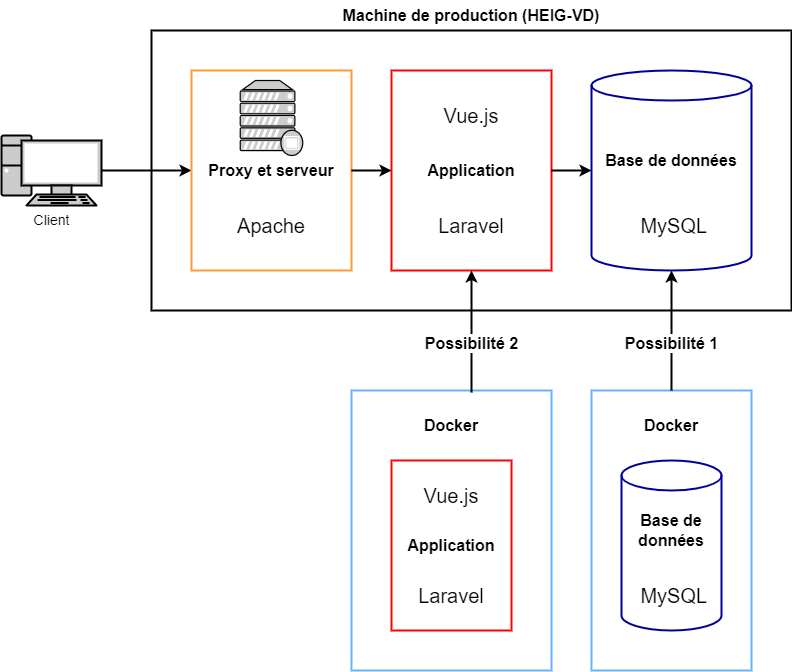
\includegraphics[width=\textwidth]{./assets/figures/infrastructure-prod-choix.drawio.png}
        \caption{Différentes possibilités d'infrastructure de production \label{infrastructure-prod-choix.drawio}}
    \end{figure}
\end{center}

Le premier changement pouvant être effectué est d'utiliser une infrastructure avec uniquement la base de données en \Gls{conteneur} \Gls{docker} et le reste installer nativement, comme montré avec la possibilité numéro 1.

Le second changement, est de passer tout l'environnement de production du \Gls{backend} sous plusieurs \Gls{conteneur}s \Gls{docker} en utilisant un \emph{Docker-compose}. Ce changement correspond à la possibilité 2. Si cela venait à être réaliser, il serait possiblement nécessaire de conteneuriser le serveur \Gls{http}.

\subsubsection{Évolutions de l'infrastructure de production possibles}
Les différentes infrastructures possibles désormais présentées, il est nécessaire de les comparer en listant les pours et les contres de chaque changement en prenant comme référentiel l'infrastructure actuelle.\\
Les deux améliorations (combinées ou non) proposées sont les suivantes:
\begin{itemize}
    \item passage du \Gls{sgbd} en machine \Gls{docker};
    \item passage du projet \Gls{laravel} (et toutes ces technologies) en machine \Gls{docker}.
\end{itemize}

\subsubsection{Passage du SGBD en conteneur Docker}
Nous allons maintenant énumérer les avantages et inconvénients d'installer le \Gls{sgbd} nativement.
Certains peuvent être les mêmes qu'énumérer dans la partie précédente. Ces derniers sont visible avec la table \ref{prod-db-native}.

\begin{table}[h]
    \begin{center}
        \caption{SGBD natif \label{prod-db-native}}
        \begin{tabularx}{1.0\textwidth} {X|X}
            Avantages                                                         & Inconvénients                            \\ \hline
            + Gestion de la BD plus facile car le SGB est installé nativement & - Demande du temps
            pour l'installation                                                                                          \\
            + Sauvegarde aisément réalisable                                  & - Configuration à réaliser à la main     \\
            + Mise en place d'un service de façon triviale                    &                                          \\
                                                                              & - Installation différente pour chaque OS \\
        \end{tabularx}
    \end{center}
\end{table}

Nous allons, maintenant, énumérer les avantages et inconvénients d'avoir le \Gls{sgbd} en \Gls{conteneur}
\Gls{docker}. Ces derniers sont visible avec la table \ref{prod-db-docker}.

\begin{table}[h]
    \begin{center}
        \caption{SGBD en conteneur Docker \label{prod-db-docker}}
        \begin{tabularx}{1.0\textwidth} {X|X}
            Avantages                                                  & Inconvénients                                                          \\ \hline
            + Accélère l'installation de l'environnement de production & - Gestion de la BD
            potentiellement plus compliquée                                                                                                     \\
            + Facilite la mise à jour de l'environnement de production si l'environnement de
            développement intègre un containeur Docker pour le SGBD    & - Sauvegarde de la BD
            potentiellement plus compliquée sans interface graphique                                                                            \\
            + Configuration en gande partie déjà réalisée              & - Mise en place d'un service non trivial                               \\
            + Compatible avec tous les OS                              & - Docker peut avoir des problèmes de performances
            \cite{labrecque}                                                                                                                    \\
                                                                       & - Nécessite Docker et les connaissances qui vont avec \cite{labrecque} \\
        \end{tabularx}
    \end{center}
\end{table}

Si nous évaluons les deux solutions proposées selon les besoins, désormais bien connus et suivants:
\begin{itemize}
    \item la performance de l'infrastructure;
    \item la simplicité de mise à jour du programme au sein de l'infrastructure;
    \item la robustesse de l'infrastructure;
    \item la flexibilité de l'infrastructure.
\end{itemize}

Nous nous rendons compte que les deux solutions se valent à peu de chose près. Je choisi donc d'essayer de mettre en place une infrastructure avec \Gls{docker} en premier temps. Si cela est trop compliqué, l'autre solution étant viable pourra toujours être utilisée.

\subsubsection{Passage de Laravel en conteneur Docker}
Passons maintenant au passage de l'environnement \Gls{laravel} en \Gls{conteneur} \Gls{docker}.

Pour ceci, nous allons énumérer les avantages et inconvénients d'installer nativement cet
environnement. Ces derniers sont visible avec la table \ref{prod-laravel-native}.

\begin{table}[h]
    \begin{center}
        \caption{Laravel natif \label{prod-laravel-native}}
        \begin{tabularx}{1.0\textwidth} {X|X}
            Avantages                           & Inconvénients                                               \\ \hline
            + Meilleur performance              & - Mise à jour compliquée si un changement de version a lieu \\
            + Gestion totale de l'environnement & - L'installation demande du temps                           \\
                                                & - Configuration à faire à la main                           \\
        \end{tabularx}
    \end{center}
\end{table}

Nous allons, maintenant, énumérer les avantages et inconvénients d'avoir l'environnement \Gls{laravel}
en machine \Gls{docker}. Ces derniers sont visible avec la table \ref{prod-laravel-docker}.

\begin{table}[h]
    \begin{center}
        \caption{Laravel en conteneur Docker \label{prod-laravel-docker}}
        \begin{tabularx}{1.0\textwidth} {X|X}
            Avantages                                                  & Inconvénients                        \\ \hline
            + Mise à jour du programme facilitée, dans tous les cas    & - Peut laisser des failles de
            sécurité, suivant l'environnement mis en place                                                    \\
            + Accélère l'installation de l'environnement de production & - Mise en place d'un service
            non trivial                                                                                       \\
            + Configuration en gande partie déjà réalisée              & - Docker peut avoir des problèmes de
            performances, \cite{labrecque}                                                                    \\
            + Offre une possibilité d'extensibilité horizontale        & - Nécessite Docker et les
            connaissances qui vont avec. \cite{labrecque}                                                     \\
        \end{tabularx}
    \end{center}
\end{table}

Si nous évaluons les deux solutions proposées selon les besoins explicité précédemment,nous nous rendons compte que la solution avec \Gls{docker} paraît plus adaptée mais la configuration des \Gls{conteneur}s pourrait être compliquée. De ce fait, la solution native, étant viable, peut également être utilisée.

\subsubsection{Résultat de l'analyse}
Suite à cette analyse des outils, la solution la plus adaptée semble être de mettre en place
l'environnement de production suivant \ref{env-prod}.

\begin{table}[h]
    \begin{center}
        \caption{Environement de production choisi \label{env-prod}}
        \begin{tabular}{c|c}
            Outil             & Technologie utilisée \\ \hline
            SGBD - MySQL      & Docker               \\
            Backend - Laravel & Docker               \\
        \end{tabular}
    \end{center}
\end{table}

La solution installant \Gls{laravel} nativement a finalement été préférée lors de la réalisation du projet par manque de connaissance et la complexité de la mise en place d'une environnement \Gls{docker} complet.

% cliffhanger
Les choix d'infrastructures réalisés, une analyse de risque de cette dernière serait nécessaire, mais je vais vous expliquer par la suite ce qui m'a empêcher d'en réaliser une.

\subsubsection{Analyse de risques}
L'analyse de risques de l'infrastructure de production est un point très important lorsque l'on publie un logiciel. Cette dernière peut être très complexe et nécessite énormément de connaissances.
Une analyse de risque complète demande une quantité conséquente de travail. L'intervention d'experts dans le domaine, via par exemple, des audits serait une solution pour réaliser cette partie du projet.\\
L'analyse de risques ne pourra donc pas être réaliser lors de ce projet, pour toutes les raisons énumérées plus haut, mais aussi car ce n'est pas le but principal de ce dernier.\\
J'ai donc décider d'appliquer tout ce que je connaissais et faire le meilleur travail possible sans aller en profondeur dans le sujet.

\clearpage

% cliffhanger
La discussion sur l'analyse de risque faite, revenons au choix qui fera le lien entre notre infrastructure de développement et de production, les \Gls{devops}.

% devops
\subsection{Pipeline DevOps}

Dans la partie suivante, nous allons parler de \Gls{devops}, si vous êtes familier avec le terme et le concept, vous pouvez sans autre sautez la section.

\subsubsection{Introduction aux Devops}

%https://blog.logrocket.com/how-to-create-a-ci-cd-for-a-laravel-application-using-github-actions/
%https://www.youtube.com/watch?v=scEDHsr3APg
%https://www.padok.fr/blog/devops-tout-savoir
%https://azure.microsoft.com/en-us/overview/what-is-devops/#devops-overview
%https://www.ibm.com/cloud/learn/devops-a-complete-guide
Pour commencer, c'est quoi les \Gls{devops}?\\
Les \Gls{devops} c'est un ensemble de processus permettant de gérer et faciliter le développement et le déploiement continu de l'application. Cela permet de garantir une meilleure qualité du code et de simplifier l'intégration de ce dernier. C'est-à-dire, si un collaborateur souhaite ajouter sa partie du code au projet, il doit d'abord passer par un système automatisé de contrôle et d'intégration de son code avant de pouvoir l'ajouter. Cette partie est appelée \Gls{ci}.\\
Les \Gls{devops} intègre également tout ce qui est déployement continu et livraison continue (\Gls{cd}).
En pratique, ils intègrent également d'autre aspect, comme la maintenance de l'infrastructure de
production et de développement, la sécurité des processus et beaucoup d'autres concepts.\\
Au final c'est un cycle de vie visant à faciliter le développement d'applications en équipe.\\
Nous peuvons observer un exemple de lifecycle fourni par IBM selon la figure \ref{devops-lifecycle}.

\begin{center}
    \begin{figure}[H]
        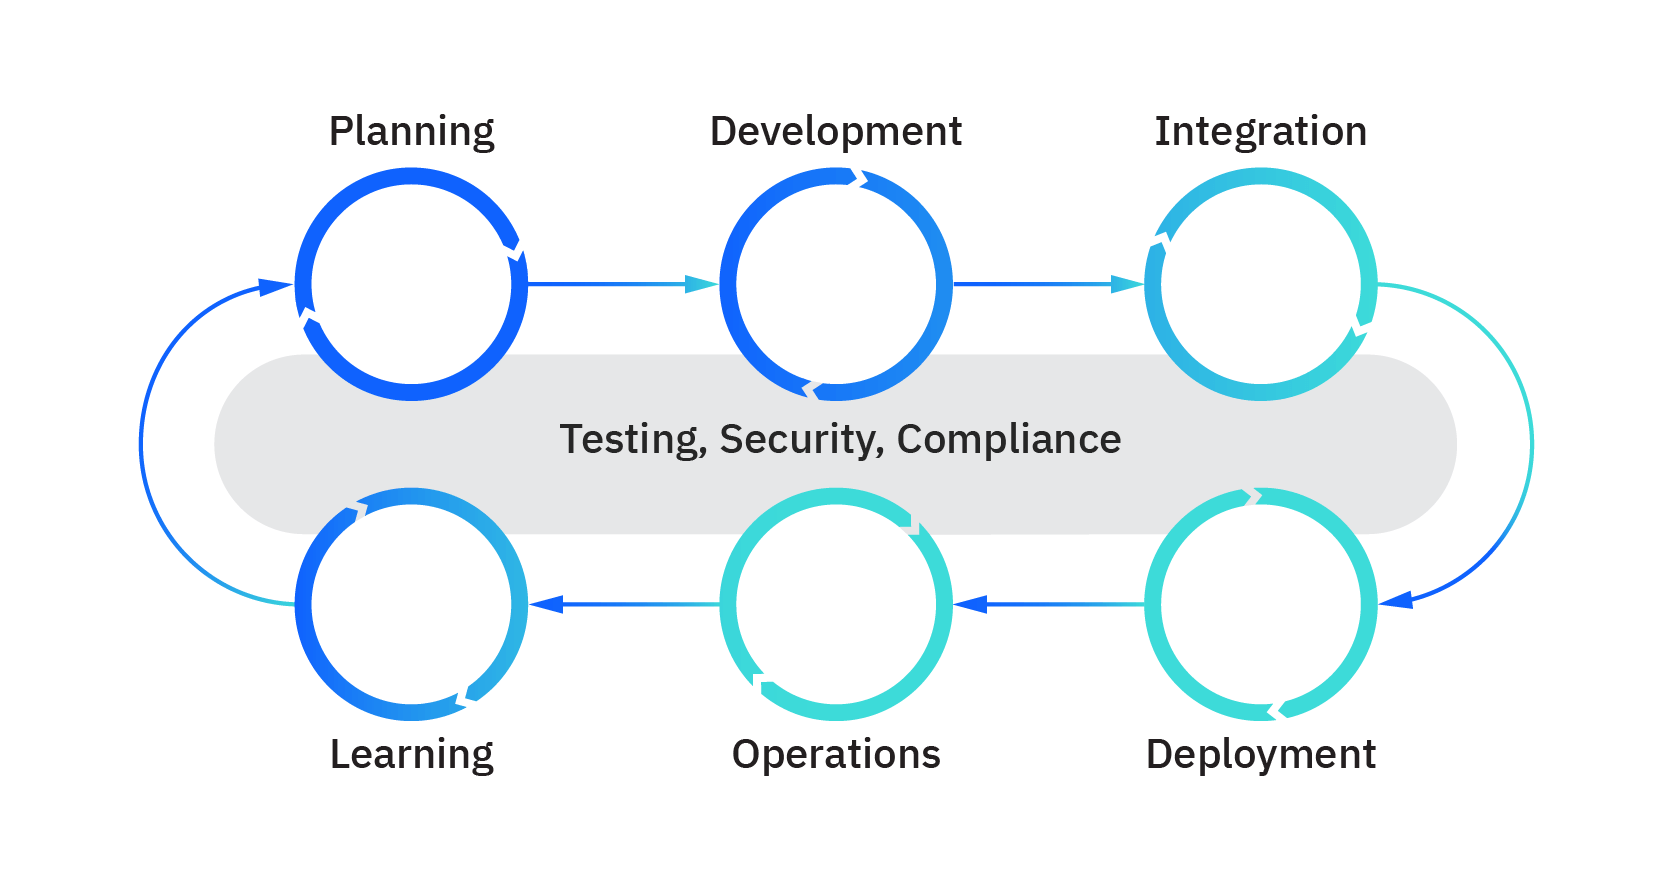
\includegraphics[width=\textwidth]{./assets/figures/ibm-devops-lifecycle.png}
        \caption[Cycle de vie de développement]{Cycle de vie de développement - IBM} \label{devops-lifecycle}
    \end{figure}
\end{center}

Aucun \Gls{devops} ou \emph{pipeline} n'avait été réalisé lors du précédent projet.\\
Nous avons donc que des propositions, sans solution existante (ce qui était le cas pour d'autres choix).\\

% cliffhanger
Avant de présenter chacun des \emph{pipeline} \Gls{devops} proposé, il est nécessaire d'expliquer pourquoi chacun de ces derniers passent par \Gls{github}, et plus précisément, les \Gls{github} Actions.

\subsubsection{Choix de GitHub}
Tout d'abord, il faut comprendre qu'il existe d'autres outil de "gestion" de \Gls{devops}, appelé
aussi services de \Gls{ci} / \Gls{devops}, en voici une liste non exhaustive:
\begin{multicols}{2}
    \begin{itemize}
        \item \href{https://www.jenkins.io/}{Jenkins};
        \item \href{https://www.jetbrains.com/teamcity/}{TeamCity};
        \item \href{https://www.guru99.com/top-20-continuous-integration-tools.html}{CircleCI};
        \item \href{https://www.travis-ci.com/}{Travis-CI};
        \item \href{https://about.gitlab.com/}{GitLab};
        \item \href{https://www.atlassian.com/software/bamboo}{Bamboo};
        \item \href{https://www.gocd.org/}{GoCD};
        \item \href{https://azure.microsoft.com/fr-fr/services/devops/}{Azure DevOps}.
    \end{itemize}
\end{multicols}

Tous ces outils, mise à part \Gls{gitlab}, doivent être installé en plus et configurer pour le projet.\\
Comme il s'agit d'un projet assez restreint et n'impliquant que peu de personnes, nous cherchons à rester dans une solution simple et donc "all in one".\\
Nous n'allons donc pas plonger dans les détails de chaque technologie citée plus haut.\\
Parmi les solutions "all in one", c'est-à-dire qui propose des services de \Gls{ci} / \Gls{devops} et permette le versioning de code, il reste uniquement \Gls{gitlab} et \Gls{github} comme choix.\\
Ne souhaitant pas réaliser une profonde analyse sur ces 2 solutions, car les 2 étant souvent considérées comme équivalentes ou interchangeable, ma connaissance de la solution \Gls{github} est un argument suffisant, selon moi, pour faire pencher la balance en sa faveur.
% Tous les outils CI / CD
%https://katalon.com/resources-center/blog/ci-cd-tools#
%https://www.lambdatest.com/blog/31-best-ci-cd-tools/
%https://www.guru99.com/top-20-continuous-integration-tools.html
%https://stackshare.io/stackups/github-actions-vs-gitlab-ci#pros

% cliffhanger
Le choix du dépôt de code fait, voyons comment nous allons réaliser la suite des \Gls{devops} avec ce dernier et quel choix nous allons faire.

\subsubsection{Présentation et comparaison des \emph{pipeline} Devops possibles}

Sur la figure \ref{devops-choix.drawio}, nous remarquons le \emph{pipeline} \Gls{devops} que nous allons utiliser mais avec 3 possibilités en ce qui concerne la façon de transférer le code entre le développement et la production. Nous allons justement parcourir ces choix dans ce chapitre.

%\figi{devops-choix.drawio}{16cm}{Différents \emph{pipeline}s DevOps possibles}
\begin{center}
    \begin{figure}[H]
        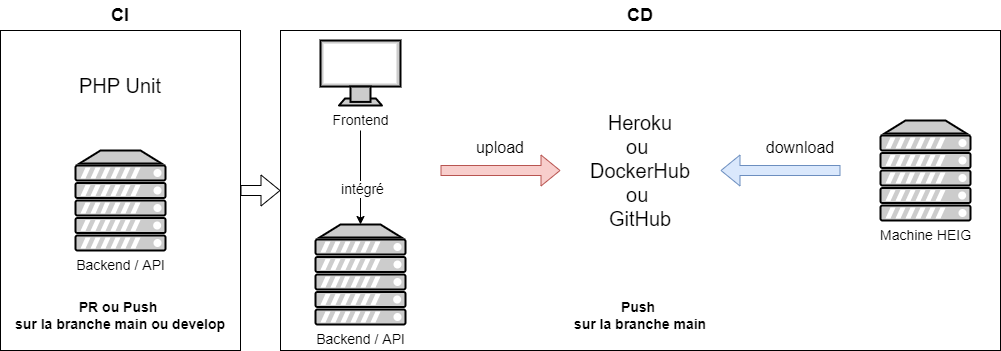
\includegraphics[width=\textwidth]{./assets/figures/devops-choix.drawio.png}
        \caption{Différents \emph{pipeline}s DevOps possibles \label{devops-choix.drawio}}
    \end{figure}
\end{center}

Le \emph{pipeline} passant par \Gls{docker} possède uniquement un intérêt si l'infrastructure de production tourne uniquement à l'aide de \Gls{conteneur}s \Gls{docker}. En effet, le but est de construire les images \Gls{docker} contenant tout ce qui est nécessaire (configurations, programmes, etc.) au niveau de la machine de développement, puis d'envoyer ces dernières sur un dépôt (\Gls{repository}) d'image, en l'occurence, \emph{Dockerhub}. Puis de
récupérer ces images sur la machine de production et de les télécharger, puis lancer.

Le second \emph{pipeline}, passerait par une plateforme appelée Heroku. Heroku permet de déployer son application sur l'un de leur serveur, puis le redéployer sur une machine de production finale.\\
Cette approche est très intéressante car l'étape intermédiaire permet de tester l'application sur une autre machine que celle de développement et ceci avant de livrer en production.\\
Le problème avec cette solution, c'est qu'il est impossible de donner des accès \Gls{vpn} à cet organisme et donc impossible de déployer sur notre machine à l'intérieur du réseau de la \Gls{heig-vd}.

Finalement, le troisième \emph{pipeline} passant uniquement par \Gls{github}, est la solution la plus simpliste en terme du nombre de technologies utilisées. Cette dernière repose sur le fait de pousser le code sur \Gls{github} et de le mettre à jour sur la machine de production via un script qui récupère les données sur le \Gls{github}.

\subsubsection{Comparaison des \emph{pipeline} Devops possibles}
Nous allons définir pour chacun des \emph{pipeline}s, les avantages et inconvénients de ces derniers.
Mais pour réaliser cette section, certains prototypes doivent être réalisés, ainsi que des recherches appronfidies sur la mise en oeuvre des différents \emph{pipeline}.\\
En effet, n'étant pas expert dans le domaine, et n'ayant pas le temps de le devenir le temps de ce travail, l'un des critères / besoins importants et la facilité de mise en place du \emph{pipeline}.

Comme le \emph{pipeline} utilisant \emph{Heroku} ne peut pas être utilisé et que le \emph{pipeline} utilisant \emph{DockerHub} n'est également pas utilisable car l'application \Gls{laravel} ne sera pas conteneurisée, il ne nous reste plus que la solution passant par \Gls{github}.

%\clearpage
%\subsection{Système de gestion de base de données}
% postgre vs mysql
%https://www.geeksforgeeks.org/difference-between-mysql-and-postgresql/
%https://www.simplilearn.com/tutorials/sql-tutorial/postgresql-vs-mysql
%https://www.ibm.com/cloud/blog/postgresql-vs-mysql-whats-the-difference
%https://stackshare.io/stackups/mysql-vs-postgresql

% upgrade to laravel 9
%https://laravel.com/docs/9.x/upgrade
%https://github.com/laravel/vonage-notification-channel/blob/3.x/UPGRADE.md

% cliffhanger
Le choix concernant les \Gls{devops} fait, il ne nous reste plus que le dernier choix concernant le système d'authentification à réaliser et nous allons voir cela dans la prochaine section.

\subsection{Système d'authentification}
Pour l'authentification, nous avions deux possibilités, utiliser le système de l'école ou utiliser \href{https://www.switch.ch/edu-id/}{Switch edu-ID}. Switch edu-ID est basé sur \href{https://www.switch.ch/aai/about/shibboleth/}{Shibboleth} et \href{https://support.google.com/a/answer/6262987?hl=fr}{SAML}, tandis que le système de l'école utilise \href{https://www.keycloak.org/}{Keycloak}.

Shibboleth a comme désavantage d'être un outil supplémentaire à ajouter à la machine de production, de ne pas être simple à mettre en place et d'être difficilement testable et utilisable en phase de développement. \\
Il possède comme avantage de toucher un plus grand nombre d'utilisateur et d'avoir déjà été mis en place lors de l'ancien travail de Bachelor.

Keycloak étant basé sur \href{https://openid.net/connect/}{OpenID}, il a comme avantage de fournir un \Gls{jwt} et d'ensuite pourvoir l'utiliser afin de vérifier l'identité de l'utilisateur grâce à une signature également fournie par Keycloak. Un formulaire de connexion / d'authentification est également fourni avec l'outil. Un autre avantage et que l'école possède une totale maîtrise de l'outil et cela facilite grandement la mise en place et collaboration. \\
L'outil a comme désavantage de restreindre l'authentification aux membres de l'école \Gls{heig-vd}.

Si vous souhaitez plus d'informations sur les différences et le fonctionnement de chacun de ses système, je vous conseille l'article suivant: \href{https://www.parallels.com/blogs/ras/oauth-vs-saml-vs-openid/#:~:text=While%20the%20use%20cases%20for,than%20SAML%20and%20OpenID%20Connect}{OAuth vs SAML vs OpenID: Learn the Differences between Them}.

%todo expliquer différences entre openID, SAML et OAuth2
%https://www.parallels.com/blogs/ras/oauth-vs-saml-vs-openid/#:~:text=While%20the%20use%20cases%20for,than%20SAML%20and%20OpenID%20Connect.

Le système d'authentification Keycloak a finalement été choisi, il me paraîssant le plus adapté et le plus facilement extensible grâce à \emph{OpenID}.

% cliffhanger
Le système d'authentification choisi, nous pouvons finalement passer dans la première partie de la réalisation du projet et plus spécifiquement comment j'ai géré mon projet et les outils que j'ai utilisés.

\chapter{Github et gestion de projet}
Avant de commencer à parler de conception et de réalisation, il est nécessaire de parler de la façon dont les projets sont stockés et gérer.

\section{Association GitHub}
La première chose réalisée est d'avoir créer une association \Gls{github} au nom du \href{https://github.com/heig-fablab}{heig-fablab}. C'est un point important car cela permet de regrouper plusieurs dépôts (\Gls{repository}) sous le même "groupe de travail", la même association.

\section{Repositories}
Dans cette association, trois dépôts ont été créés, les voici:
\begin{itemize}
    \item \href{https://github.com/heig-fablab/fablab-manager}{fablab-manager} étant le dépôt principal contenant le \Gls{backend} et le \Gls{frontend} compilé et minimisé pour la production;
    \item \href{https://github.com/heig-fablab/fablab-manager-frontend}{fablab-manager-frontend} étant le dépôt contenant le code du {frontend};
    \item \href{https://github.com/heig-fablab/heig-keycloak-auth-token}{heig-keycloak-auth-token} étant un dépôt permettant de faciliter le développement du \Gls{backend}.
\end{itemize}

\section{README}
Chaque dépôt contient un fichier \emph{README.md} indiquant toutes les instructions à suivre afin d'installer l'environement de développement lié au dépôt ainsi que quelques informations supplémentaires utiles tel que les versions des outils utilisés pour le développement.

Les dépôt sont rédigés en anglais afin de pouvoir transmettre le plus aisément possible le projet.

\section{Wiki}
Le dépôt \emph{fablab-manager} étant le principal, ce dernier possède également un wiki avec énormément d'informations concernant la conception et la réalisation du projet. On peut notamment retrouver une majorité des informations disponibles dans ce rapport.

\section{Issues Github}
Ce dépôt liste également toutes les tâches réalisées et à réaliser du projet. Ces tâches sont répertoriées sous forme d'\emph{issue} \Gls{github}. Ces dernières indique grâce à des labels s'il s'agit d'un bug, de la documentation, un ajout, etc. et si elles appartiennent au projet \Gls {frontend} ou \Gls{backend} ou les deux.

\section{Kanban}
Les \emph{issues} abordées, il est maintenant nécessaire de parler du \emph{kanban} mis en place. Le \emph{kanban} est un tableau contenant toutes les \emph{issues} et les rangeants dans des catégories en fonction de l'avancement de la tâche / \emph{issue}. \\
Le \emph{kanban} que j'ai créé contient 5 colonnes:
\begin{itemize}
    \item \emph{backlog} représantant toutes les tâches / \emph{issues} à mettre en place sur le projet à terme;
    \item \emph{todo (actual sprint)} représantant toutes les tâches / \emph{issues} à réaliser pendant le sprint actuel;
    \item \emph{in-progress} indiquant toutes les tâches / \emph{issues} en cours de réalisation,
    \item \emph{done but can be modified} indiquant les tâches / \emph{issues} terminée mais pouvant être re-modifiée;
    \item \emph{done} représentant les tâches / \emph{issues} terminées et fermées.
\end{itemize}

\section{Milestones}
Pour m'organiser et travailler d'une manière agile, j'ai créé des milestones représantant les sprints que j'allais réaliser durant le projet. Une milestone spécial s'y est glisser, elles est nommée \emph{nice to have} est représente toutes les tâches non inclues dans le cahier des charges ou non prioritaires / nécessaires mais étant intéressantes à ajouter au projet.

\section{Git flow / Workflow}
Même si j'étais seul lors de ce projet, j'ai prévu qu'il soit potentiellement maintenu par plusieurs personnes à la fois, j'ai donc établi un \Gls{git} flow ou Workflow afin de faciliter la collaboration. Ce dernier suit un standard bien établi et est consultable à la figure
\ref{git-flow} tiré dur site \href{https://www.atlassian.com/fr/git/tutorials/comparing-workflows/.gitflow-workflow}{atlassian}.

\begin{center}
    \begin{figure}[h]
        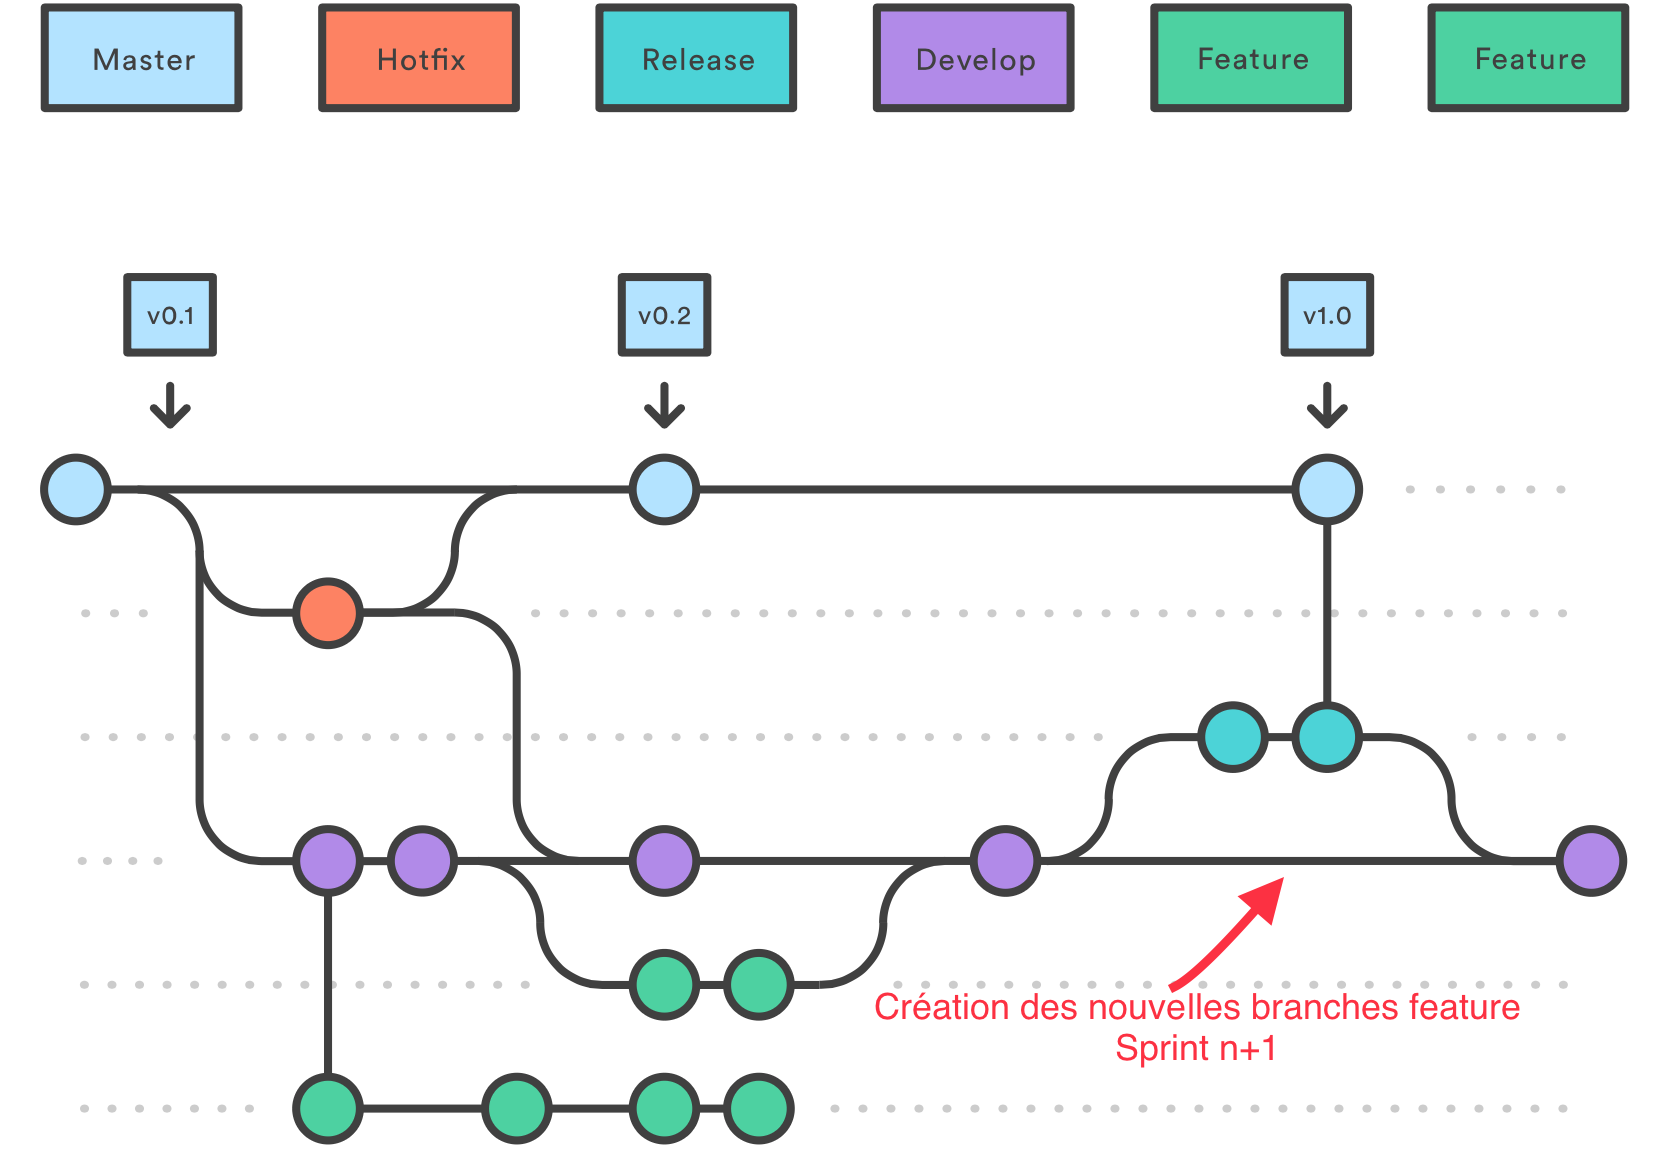
\includegraphics[width=\textwidth]{./assets/figures/git-flow.png}
        \caption{Git flow \label{git-flow}}
    \end{figure}
\end{center}

\section{Postman}
Durant le développement du \Gls{backend}, j'ai réalisé un \href{Postman collaboratif}{https://www.postman.com/} afin d'acceuillir toutes les requêtes possibles pour le \Gls{backend} et le tester pendant la phase de développement.

% cliffhanger


\section{Planning}
%todo
Cette section a pour but d'apporter une discussion sur le planning et son évolution.
Les deux versions (initiale et finale) du planning sont disponibles en annexe.

\subsection{Description générale du planning}

Dans le document, certaines couleurs apparaîssent, en voici les significations:
\begin{itemize}
    \item le gris indique la semaine du \emph{CRUNCH};
    \item le orange foncé indique la semaine de vacances de Pâques;
    \item le bleu indique quand les tâches seront réalisées;
    \item le orange clair indique les tâches réalisées tout au long du projet;
    \item le vert indique la marge d'erreur / d'imprévus;
    \item en rouge, les rendus / jalons importants du projet.
\end{itemize}

La semaine sans travail est un choix personnel, cette semaine là, nous avons une semaine spéciale à la \Gls{heig-vd}, le \emph{CRUNCH}. C'est une semaine interdisciplinaire obligatoire.

Il faut savoir qu'il y aura sûrement une grande différence entre la réalisation des tâches indiquées
et la réalité. En effet, dans les projets comme celui-ci, il est souvent nécessaire de jongler entre
les différentes tâches et il est donc compliqué de suivre un planning en cascade comme ce dernier.

Le planning est séparé en trois grandes parties:
\begin{itemize}
    \item l'analyse;
    \item la conception et la réalisation;
    \item la préparation des livrables.
\end{itemize}

La conception et réalisation ne sont pas séparées car je vais devoir altérner entre les deux.
Je vais souvent concevoir quelque chose, le réaliser, me rendre compte que ce n'est
pas optimal et répéter le processus. C'est pour cela que ces deux parties sont liés et non séparées.
Cela permet de travailler itérativement, comme cela se fait beaucoup en développement logiciel.

\subsection{Analyse}
L'analyse contient principalement de l'étude et des choix technologiques. Certains prototypes peuvent être réalisé pour consolider les choix effectués. Tous les choix technologiques et conceptuels sont cruciaux pour la suite du projet.\\
La justification des choix à l'aide d'articles scientifiques sera également un point à ne pas négliger au niveau du temps consacré.

\subsection{Conception et réalisation}
La partie conception et réalisation est séparée en plusieurs sections:
\begin{itemize}
    \item Environnement de développement et de production;
    \item \Gls{devops};
    \item Modification du \Gls{backend} et de la base de données;
    \item Modification du \Gls{frontend}.
\end{itemize}

Les points à ne pas sous-estimer dans ces parties sont la mise en place d'un bon environnement de travail / de développement et la \Gls{ci} pour la première partie du projet. Ces deux points sont essentiels pour pouvoir développer l'application sans problème.\\
Deux sujets sur la conception peuvent prendre du temps et sont très important, il s'agit de la conception de la base de données, car celle-ci découle sur toute la réalisation du \Gls{backend} et la conception de l'architecture de code, car si elle est significativement changée au milieu du projet, peut faire perdre énorméement de temps.\\
Un point qui a été mal identifié de ma part lorsque j'ai réalisé la première version de ce planning,
c'est le fait que concevoir toute une nouvelle base de données allaient presque m'obliger à
re-développer le \Gls{backend} quasiment de zéro sans pouvoir utiliser significativement le travail déjà
présent.\\
Cette partie était presque prévue sous le point "Séparation et refactor du code déjà écrit" mais
elle prendra beaucoup plus de temps que prévu. Elle va s'en doute s'étendre à plus de 80 heures de
travail. C'est pourquoi elle a été séparée en plus petite partie. \\
Pour finir, cette partie est cruciale pour le projet car elle correspond à la base de l'\Gls{api} et doit être solide pour pouvoir itérer dessus. \\
Le dernier point dont j'avais sous-estimer et oublier dans ma première version du planning, était le déploiement, j'ai donc également rajouté cette partie à ma dernière version du planning.

\subsection{Livrables}
En ce qui concerne la préparation des livrables, il est clair que le rapport est l'un des points
demandant le plus de temps au niveau du travail et est crucial pour la réussite du projet. Ce
dernier se réalisant tout au long du projet, il n'a pas de date précise où il va être réaliser. On
peut cependant prévoir plus d'effort avant le rendu intermédiaire et le rendu final.\\
En ce qui concerne la présentation de la défense, elle est indiquée sur le planning mais sera uniquement réalisée pendant le mois d'août.\\
La partie gestion de projet est également et logiquement réalisée tout au long du projet.

\subsection{Discussion sur le planning}
En observant le planning finale, nous remarquons, tout d'abord, que mes heures de travail ne suivent pas du tout la courbe prévue et cela était à prévoir et est totalement normale que cela soit comme ça. En effet, dans les projets de développement, il est difficile de réaliser une tâche après l'autre, car nous sommes souvent amené à réaliser plusieurs tâches à la fois.

Ensuite, nous nous rendons compte que j'ai mis beaucoup plus de temps prévu pour le écrire le rapport, ainsi que pour le déploiement. Cela se remarquera encore dans les problèmes rencontrés et expliqués plus tard dans le rapport. L'installation des technologies a également pris plus de temps que prévu avec tous les problèmes rencontrés à cause de \emph{WSL}.

Au niveau des tâches ayant pris moins de temps que prévu, nous avons les différentes tâches liées au choix, mais cela peut s'expliquer par une mauvaise répartition dees heures notées entre le rapport sur ce sujet et ces choix en eux-même. \\
La création des containeurs \Gls{docker} a également pris moins de temps que prévu car j'en ai réalisé moins que prévu. \\
Quand à l'installation des technologies et la machine virtuelle, les heures ont dû être mal répartie avec le déploiement au niveau du suivi. \\
J'ai gagné beaucoup de temps au niveau de la \Gls{cd} car aucune n'a été créée finalement, seul un guide a été écrit et cela a pris beaucoup moins de temps.
Nous remarquons que les routes \emph{messages} et \emph{users} ont pris moins de temps que prévu et c'est une bonne chose. \\
Les tests unitaires m'ont également pris moins de temps que prévu et ceci car le nombre est assez limité. \\
Finalement, nous remarquons également que je n'ai pas eu le temps de passer énormément de temps sur la configuration des webosckets côté \Gls{frontend}.

Au final, je m'en suis plus tôt bien sorti au niveau de l'estimation des heures du travail tout en maintenant et faisant évolué ce planning tout au long du projet.

% cliffhanger
Maintenant les outils de travail ont été définis, nous pouvons passer à la conception et la réalisation de la base de données, racine de tout projet avec stockage de données.

\chapter{Conception et Réalisation de la BD}

\section{Modèle EA}
Le modèle Entité-Associations est la première étape lors de la conception d'une base de données. Il se rapproche également d'un diagramme de classe classique utiliser pour la \emph{POO} (programmation orienté objet).\\
Nous allons décrire chacune des entités et ses relations.\\
Mais avant cela, voici quelques informations sur le schéma, une sorte de légende:\\
Un rectangle représente une entité et possède son nom dans sa partie supérieur.\\
Les valeurs textuelles en dessous sont les champs de l'entité. Le champ souligné représente la clé primaire de l'entité, cette dernière doit être unique.\\
Les traits tiré entre deux entités sont des associations et peuvent se lire dans les deux sens. Les verbes écrits au dessus des traits servent à donner un sens à l'association.\\
Les symboles et numéros à chaque extrémités des entités indiquent respectivement:
\begin{itemize}
    \item 0 : zéro / aucun;
    \item 1 : un;
    \item 1..* : un ou plusieurs;
    \item * : zéro ou plusieurs.
\end{itemize}

Par exemple, nous peuvons lire l'association \emph{user - message}, comme ceci:\\
Un utilisateur peut envoyer zéro ou plusieurs messages.\\
Un message peut être envoyé que par un utilisateur.

Finalement, quelques commentaires peuvent être ajouté avec des rectangles pliés en haut à droite et relié avec des traits pointillés.

\begin{center}
    \begin{figure}[H]
        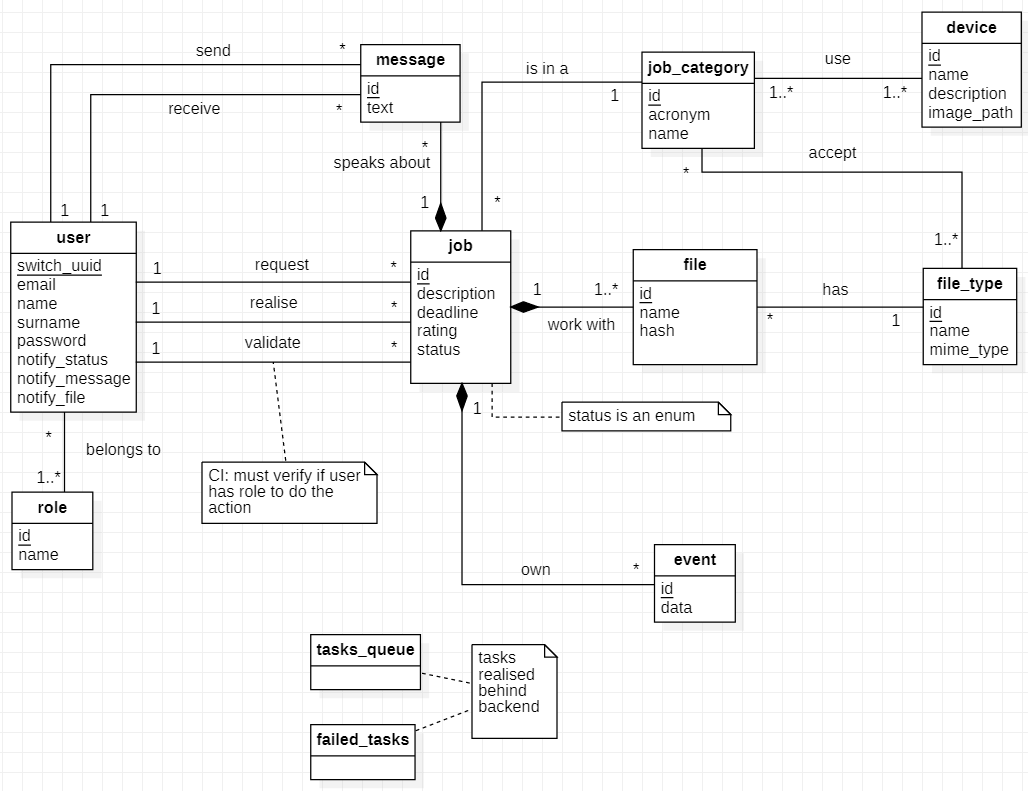
\includegraphics[width=\textwidth]{./assets/figures/ea.png}
        \caption{Modèle EA \label{ea}}
    \end{figure}
\end{center}

\subsection{Entité users}
L'entité \emph{user} représente un utilisateur de l'application, que ce soit un élève, un professeur ou un technicien.\\
Il possède des informations classiques le concernant, ainsi que le champ \emph{username} représentant l'identifiant unique fourni par le service Switch edu-id qui sera utilisé.\\
Les champs contenant le mot \emph{notify} servent à stocker les préférences de l'utilisateur concernant les notifications de l'application.

Nous voyons au niveau des relations, que l'utilisateur peut envoyer et recevoir des messages.\\
Il peut posséder également plusieurs rôles mais doit en posséder au moins un, celui par défaut qui est le rôle \emph{client}.\\
L'utilisateur peut de toute façon faire une demande de travail (job). Cependant, seul les utilisateurs possédant le rôle \emph{validator}, en général, les professeurs pourront valider le travail.\\
Le travail validé, un \emph{worker}, en général un technicien, pourra réaliser le travail demander et en indiquer le suivi.

\subsection{Entité jobs}
L'entité \emph{job} représente un travail demandé par un utilisateur de l'application.\\
Il possède un id (identifiant unique), un titre, une description du travail à réaliser, une date butoir (deadline), une évaluation que l'utilisateur / client qu'il peut attribuer au travail terminé, le nombre d'heures passées à réalisé le travail et un status d'avancement du travail mis à jour par le travailleur.\\
Le status d'avancement d'un travail sera défini par un enum (liste exhaustive de valeurs), la voici:
\begin{itemize}
    \item new;
    \item validated;
    \item assigned;
    \item ongoing;
    \item on-hold;
    \item completed.
\end{itemize}

Nous voyons au niveau des relations, que le travail peut posséder des messages qui lui sont liés.\\
Il possède également une catégorie de travail définissant les machines qui peuvent être utilisées pour le réaliser.\\
Le travail possédera également un utilisateur client, un validateur et un travailleur.\\
Il doit également contenir un ou plusieurs fichiers nécessaires pour réaliser le travail demandé.\\
Finalement, certains événements peuvent être lié au travail. Nous parlons ici d'événements permettant de préfevenir l'utilisateur via des notifications ou email.

\subsection{Entité roles}
L'entité \emph{role"}représente simplement un rôle que peut avoir un utilisateur au sein de l'application. Cette entité est nécessaire car un utilisateur peut posséder plusieurs rôles et ils doivent tous être défini la même chose.\\
Seul un id (identifiant unique) et un nom du rôle est nécessaire.\\
Voici la liste des rôles définis:
\begin{itemize}
    \item admin;
    \item client;
    \item worker;
    \item validator.
\end{itemize}

\subsection{Entité messages}
L'entité \emph{message} représente un message envoyé entre deux utilisateurs au sujet d'un travail demandé.\\
Il possède uniquement un id (identifiant unique) et un texte.\\
Il est associé à deux utilisateurs, un représentant celui qui a envoyé le message et l'autre celui qu'il l'a reçu. Le message est également associé au travail dont il est le sujet.\\
Une aggrégation a été modélisé pour cette dernière association car nous souhaitons supprimé tous les messages liés à un travail, si ce dernier est supprimé.

\subsection{Entité job\_categories}
L'entité \emph{job-category} représente une catégorie de travail pouvant être effecutée au Fablab, par exemple, une impression 3D ou une découpe laser.\\
La catégorie possède un id (identifiant unique), un acronyme, une description plus précise et un nom.\\
Elle est associé à un travail car ce dernier est obligé d'avoir une catégorie.\\
Elle possède également un fichier car ce dernier correspond à l'image affichée au niveau de l'interface graphique et la représentant. \\
Elle possède une liste de type de fichiers acceptés pour réaliser un travail de cette catégorie et est défini par l'association \emph{job-category - file-type}. Cela permettra de facilement vérifier si un fichier donné pour un travail peut être accepté pour la catégorie de ce dernier.

\subsection{Entité file\_types}
L'entité \emph{file-type} représente un type de fichier que peut accepter une catégorie de travail du \Gls{fablab}.\\
Le type de fichier possède un id (identifiant unique), un nom et un \href{https://developer.mozilla.org/fr/docs/Web/HTTP/Basics_of_HTTP/MIME_Types}{mime-type} étant utiliser pour valider les fichiers télécharger.\\
Comme expliqué précédement dans la catégorie, un type de fichier possède une ou plusieurs catégories qui sont acceptées.\\
Le type de fichier peut également être associé à plusieurs fichiers.

\subsection{Entité files}
L'entité \emph{file} représente un fichier fourni pour réaliser un travail du \Gls{fablab}.\\
Le fichier possède un id (identifiant unique), un nom, son dossier où il est stocké et un hash de son contenu.\\
Il est associé à un type de fichier (\emph{file-type}), ce qui est utile pour faire le lien avec la catégorie du travail.\\
Il possède évidemment un travail indiquant auquel il appartient.\\
Une aggrégation a été modélisée pour cette dernière association car nous souhaitons supprimé tous les fichiers liés à un travail, si ce dernier est supprimé.

\subsection{Entité events}
L'entité \emph{event} représente un événement concernant un travail du \Gls{fablab}. Par exemple, un événement est généré si le status d'un travail a été modifié ou si un fichier a été ajouté. \\
L'événement possède un id (identifiant unique), un champ indiquant s'il faut notifier l'utilisateur (\emph{to\_notify}), des données (\emph{data}) et une énumération contenant les valeurs suivantes:

\begin{itemize}
    \item file;
    \item message;
    \item status.
\end{itemize}

Le champ \emph{data} ne contiendra des données uniquement si l'événement est de type \emph{status} ou \emph{file}.

Il est associé à un travail comme expliqué plus précédement.\\
Il est également associé à un utilisateur afin de connaître quel utilisateur notifié si ceux dernier n'a pas consulté le travail lié à l'événement.\\
Une aggrégation a été modélisée pour cette dernière association car nous souhaitons supprimé tous les événements liés à un travail, si ce dernier est supprimé.

\subsection{Entité tasks-queue et failed-tasks}
Ces entités ont été modélisées pour effectuer les tâches en arrière plan du \Gls{backend}, comme l'envoi d'email retardé. Je ne peux pas donner plus de précisions sur les champs car ils ont été générées automatiquement.

\newpage

\section{MLD}
Le modèle logique des données n'est rien d'autre qu'une évolution du modèle EA.\\
Les entités deviennent des tables et les associations des relations, ce qui est presque la même chose.\\
Les tables sont au pluriel pour respecter la philosophie de \Gls{laravel} et de son \Gls{orm} \emph{Eloquent}.\\
Les champs obtiennent des types représentant la façon dont ils seront stockés.\\
Les clés étrangère issues des association s'ajoutent aux tables.\\
Les associations N à N du modèle EA voient naître une table intermédiaire. Voici celles qui ont été créées:
\begin{itemize}
    \item file\_type\_job\_category;
    \item role\_user.
\end{itemize}

\begin{center}
    \begin{figure}[H]
        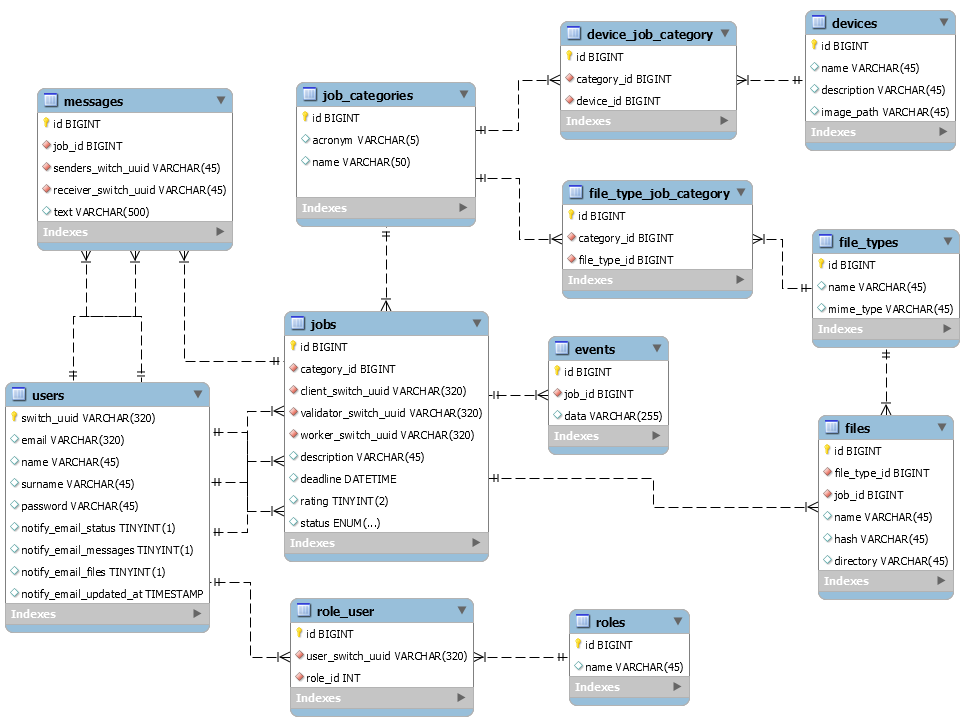
\includegraphics[width=\textwidth]{./assets/figures/mld.png}
        \caption{Modèle Logique des données \label{mld}}
    \end{figure}
\end{center}

Sur le schéma, quelques nouveaux symboles apparaîssent, voici une légende:
\begin{itemize}
    \item clé jaune : clé primaire de la table;
    \item losange bleu : la colonne ne peut pas valoir null;
    \item losange vide : la colonne peut valoir null;
    \item losange rouge : la colonne possède une clé étrangère.
\end{itemize}

Une clé étrangère étant le champ représantant une autre table issue d'une relation existante. La clé primaire représente la table en elle-même, elle est son identifiant.

\subsection{Champs spéciaux}
Quelques champs obtiennent des valeurs précises et méritent une explication.\\
Le champ \emph{username} de la table \emph{users} contient au maximum 17 caractères, car l'école défini ces nom d'utilisateurs en utilisant les 8 premières lettres du prénom et les 8 premières du nom avec un \emph{.} entre deux.
Le champs \emph{email} de la table \emph{users} possèdent 255 charactères car un email peut contenir au maximum 255 charactères \cite{email-length}.

Le champ \emph{status} de la table \emph{jobs} et le champ \emph{type} de la table \emph{events} est une enum comme expliqué précédement dans le modèle EA.

Tous les champs \emph{created\_at}, \emph{updated\_at} et \emph{deleted\_at} sont des champs automatiquement généré par \Gls{laravel} si nous ajoutons certaines options à la table et au modèle comme nous allons le voir plus tard. Ces champs indique l’heure à laquelle la donnée à été créée / modifiée / supprimée pour la dernière fois.

Les types de champs et leur taille de la base de données ont été minutieusement choisi afin de correspondre au mieux aux besoins de l'application. \\
Il a été décidé que seul 50 caractères suffiront pour stocker les noms et prénoms des utilisateurs. \\
Pour tous les autres champs ayant le nom \emph{name}, il a été observé quel était la longueur maximale possible avec les données qui nous étaient fournies et un supplément a été ajouté. \\
Le champ \emph{mime\_type} a fait l'objet d'une recherche afin de valider sa longueur maximum grâce au poste \cite{mime-type-length}. \\
De même pour le champ \emph{name} de la table \emph{file\_type} qui a été validé grâce au poste suivant \cite{extension-length}. \\
Le dernier champ à être été validé est celui nommé \emph{hash} de la table \emph{file}, ce dernier a été validé grâce au poste \cite{hash-256-length}.

% cliffhanger
Le modèle logique des données établi, il est maintenant nécessaire de l'implémenter grâce aux migrations de \Gls{laravel} et nous allons voir cela tout de suite.

\section{Migrations Laravel}

Les migrations du \Gls{backend} réalisées avec Laravel et l'\Gls{orm} \emph{Eloquent} se rapprochent le plus possibles du \emph{MLD} présenté précédement.

\subsection{Types de champs}
Voici une liste des types possibles et utilisées:
\begin{itemize}
    \item id: un entier positif incrémentable, unique, indiqué comme clé primaire et référencé via un index;
    \item string: une chaîne de caractères;
    \item longText: un grand texte;
    \item enum: une liste exhaustive de valeurs possibles;
    \item tinyInteger: un petit entier;
    \item date: une date.
\end{itemize}

La liste plus complète peut être consultée dans la doc \href{https://laravel.com/docs/9.x/migrations#available-column-types}{Laravel}.

Sur la figure \ref{migrations-jobs}, nous pouvons observer un exemple de migration contenant presque tous les points abordés ci-dessous.

\begin{listing}[h]
    \inputminted{php}{assets/code/16_create_jobs_table.php}
    \caption{Migration de la table \emph{file-types} \label{migrations-jobs}}
\end{listing}

\subsection{Champs possiblement \emph{null}}
La possibilité de laisser une valeur nulle sur un champ n'apparaît pas sur le MLD, mais est bien présente au niveau des migrations et modèles de \Gls{laravel}.\\
Tous ces champs possèdent l'indiquation: \emph{->nullable()}.\\
Seul certains champs peuvent être \emph{null} dans notre base de données et ceux-ci interviennent surtout dans la table \emph{jobs}.\\
Les champs qui peuvent être \emph{null} sont des champs dont la valeur n'est pas obligatoirement présente à la création mais peut-être ajoutée plus tard. Il s'agit par exemple de la note donnée au travail \emph{rating} ou encore le technicien devant effectuer ce dernier qui peut être assigné après coup.

\subsection{Champs uniques}
Il est possible d'indiquer qu'un champ doit posséder une valeur unique avec l'option: \emph{->unique()}.\\
Cette possibilité est par exemple utilisée par le champ email.

\subsection{Champs timestamps}
Les champs de type \emph{->timestamps()} sont un raccourci utilisé par \Gls{laravel} pour créer deux champs indiquant la date de création de la donnée et la date de modification. Ces champs sont gérés automatiquement par \Gls{laravel}, ce qui est bien pratique.

\subsection{Indexes}
Il est possible de créer des indexes sur certains champs afin d'améliorer les performances de la base de données lors de certaines requêtes. Ces indexes peuvent être créer grâce à l'instruction \emph{index('table-champ')}.\\
Ces derniers sont toujours créer sur les clés primaires et doivent être créer sur les clés étrangères. D'autres champs régulièrement utilisés par des requêtes peuvent faire l'objet d'indexes.

\subsection{Clés étrangères}
Les clés étrangères peuvent être gérées de deux façon différentes.\\
Soit nous ajoutons un champ \emph{foreignId('table-id')} suivi d'un \emph{->constrained('table')} qui permet de faire le lien directe entre la clé primaire et la clé étrangère tout en générant un index. Mais ceci est possible uniquement si nous utilisons une clé primaire de type \emph{id()}.

Dans le deuxième cas, lorsque nous possèdons une clé primaire basée sur un autre type de champ, il faut tout d'abord créer un champ à la main avec la valeur voulue.\\
Puis faire le lien entre la clé primaire et étrangère à la main en utilisant d'abord \emph{->foreign('table-champ')}, puis en référançant avec \emph{->references('champ')->on('table')}.\\
Puis, finalement, créer un index avec \emph{index('table-champ')} sur le champ de la clé étrangère.

\subsection{Options de suppression}
Des options de suppression sont proposées par \emph{Eloquent} afin de ne pas supprimer définitivement les données de la base de données, mais de simplement les désactiver afin quelles n'apparaîssent plus dans les requêtes.\\
Ceci est possible en ajoutant l'option \emph{->softDeletes()} à la table.\\
\Gls{laravel} s'occupera ensuite de gérer les cas de suppression lui-même.

% cliffhanger
Maintenant la base de données créée, parlons des données qu'il faut au minimum y ajouter et plus précisément le \emph{seeding}.

\section{Seeding de la BD}
Le \emph{seeding} de la base de données a été en s'aidant de \href{https://laravel.com/docs/9.x/seeding}{la documentation officielle de \Gls{laravel}}. \\
Deux types de \emph{seeders} ont été mise en place, la première concerne toutes les données nécessaires au bon fonctionnement du programme, que cela soit en production ou en développement. Ces données  concerne les tables suivantes:
\begin{itemize}
    \item file\_types;
    \item job\_categories;
    \item file\_type\_job\_category;
    \item roles;
    \item files;
    \item users;
    \item role\_user.
\end{itemize}

Les tables \emph{roles} et \emph{role\_user} sont nécessaire pour ajouter les utilisateur administrateur de base.

Tous les autres \emph{seeders}, donc ceux du deuxième type, sont uniquement executé en environnement de développement et ont pour but de créer quelques données fictives.

\chapter{Conception et Réalisation du Backend / de l'API}

La première chose à noter dans cette section, c'est que la version 8 était utilisée dans le précédent projet et cette dernière a été mise à jour pour utiliser la dernière version, la version 9.

% cliffhanger
Maintenant la base de données créée et peuplée, parlons de l'architecture de code que nous devons mettre en place pour intéragir avec ces dernières.

\section{Architectures de code}

Ne connaissant pas le \Gls{framework} \Gls{laravel} à l'origine, mais plutôt celui de \emph{Java Spring}, j'ai effectué un schéma de l'architecture de code de ce dernier afin de le comparer avec celui de \Gls{laravel} et pouvoir mieux le comprendre. Sur la figure \ref{architecture-code-spring}, nous voyons clairement l'architecture classique allant de la vue passant par les \emph{Controllers}, puis les \emph{services} contenant la logique métier et finalement les \emph{repository} utilisant les \emph{DAO} pour commumiquer avec la base de données. \\
Des \emph{DTO} peuvent également être ajoutées entre la vue et les controllers.

%\figi{architecture-code-spring.drawio}{16cm}{Architecture de code du framework Spring "classique"}
\begin{center}
    \begin{figure}[H]
        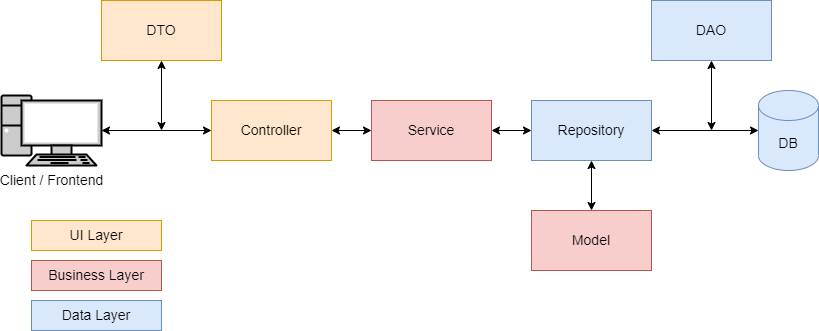
\includegraphics[width=\textwidth]{./assets/figures/architecture-code-spring.drawio.png}
        \caption{Architecture de code du Framework Spring "classique" \label{architecture-code-spring}}
    \end{figure}
\end{center}

J'ai ensuite essayé de comprendre l'architecture de code de \Gls{laravel} en me plongeant dans la documentation. \\
Je me suis rendu compte que \Gls{laravel} proposait énormément de classes ou d'outils de code que ce que j'avais pu comprendre en premier lieu. J'ai donc réaliser un schéma de l'architecture de code que je vais utiliser pour ce projet disponible sur la figure \ref{architecture-code-finale}.

%\figi{architecture-code-finale.drawio}{16cm}{Architecture de code Laravel finale}
\begin{center}
    \begin{figure}[H]
        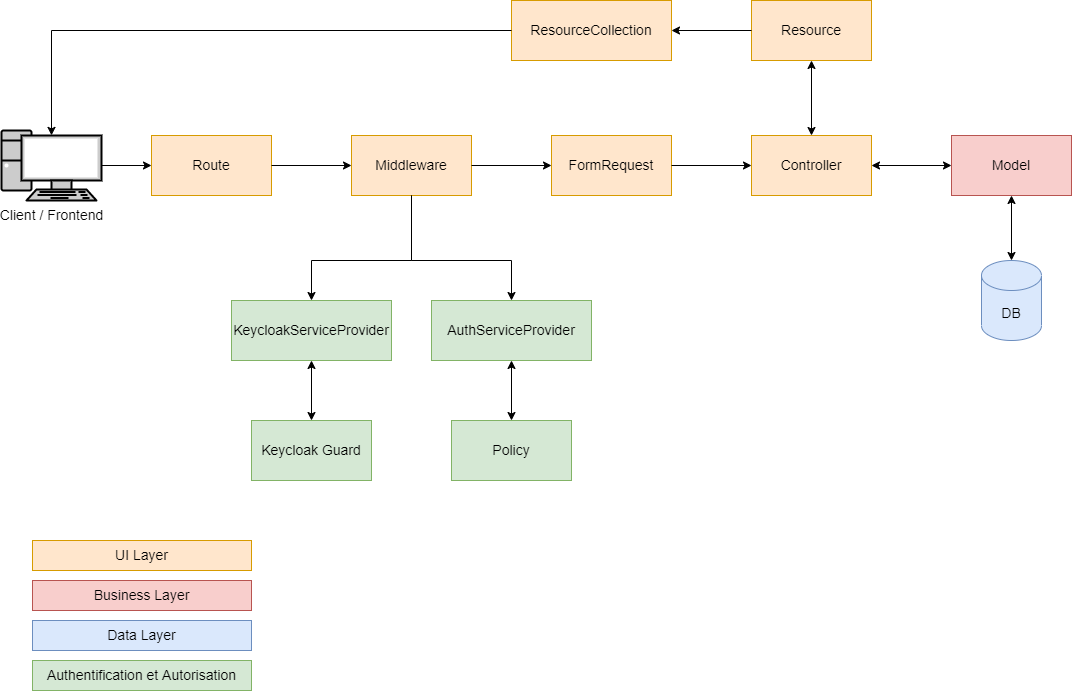
\includegraphics[width=\textwidth]{./assets/figures/architecture-code-finale.drawio.png}
        \caption{Architecture de code Laravel finale \label{architecture-code-finale}}
    \end{figure}
\end{center}

Nous allons maintenant discuté de quelques \emph{pattern} de code utilisé et fourni par \Gls{laravel}.\\
Tout d'abord, nous pouvons observer que les authorisations peuvent être contenue dans un \emph{middleware} utilisant au final des \emph{Policy} afin de contenir la logique déterminant si l'utilisateur possède le droit d'accès à une ressource.

Ensuite, nous observons que les \emph{Controllers} recevoivent des \emph{Form Rquests} représentant des requêtes contenant les valeurs nécessaires pour la requête. Les valeurs à l'intérieur des requêtes seront exhaustivement définies et syntaxiquement validées. Cela permettra de travailler avec des valeurs sûrs au niveau des \emph{Controllers} et des \emph{Models}. \\
Ces \emph{Form Rquests} peuvent être comparées à des \emph{DTO} de validation. \\
%Par exemple, il sera possible de valider qu'un email donné soit un email syntaxiquement correct.

Les \emph{Controllers} travailleront avec des \emph{Resources} (ressources) afin de retourner uniquement les valeurs voulues. Ces \emph{Resources} définissent exactement les données qui doivent être renvoyer à l'utilisateur. \\
Ces \emph{Resources} utilisent également des \emph{ResourcesCollection} permettant de
définir des collections de ressources lorsqu'une route doit fournir plus qu'un seul élément. \\
Ces \emph{Ressources} peuvent être comparées à des \emph{DTO} de sortie. \\
%Il sera par exemple possible de définir que le mot de passe de l'utilisateur ne soit
pas retourné à ce dernier. \\

% cliffhanger
Avant de passer aux détails d'implémentation de cette architecture de code, il est nécessaire de définir les routes que l'\Gls{api} fournit.

\section{Routes}

%todo must be here
\begin{listing}[H]
    \inputminted{php}{assets/code/api-1.php}
    \caption{Routes de l'API \label{routes-api-2}}
\end{listing}

\begin{listing}[H]
    \inputminted{php}{assets/code/api-2.php}
    \caption{Routes de l'API \label{routes-api-1}}
\end{listing}

\newpage

Les routes définies par l'\Gls{api} sont organisée par modèle / ressource et sont ensuite trier par action possible. \\
Voici la liste des ressources sur lesquels certaines actions peuvent être exécutées:
\begin{itemize}
    \item files;
    \item file types;
    \item job categories;
    \item jobs;
    \item messages;
    \item users.
\end{itemize}

Le détail de ces routes est consultable sur les figures \ref{routes-api-1} et \ref{routes-api-2}.

Nous remarquons aisément que la route principale est la route \emph{jobs} et que toutes les autres routes sont également liées à cette dernière. Nous pouvons également remarquer que la route \emph{file types} est uniquement réservé aux administrateurs.

\subsection{REST}
Les routes fournies essaient au maximum de suivre le principe \Gls{rest}. \\
Toutes les routes indiquant la méthode \emph{GET} servent uniquement à récupérer des informations.
Les routes avec la méthode \emph{POST} à créer une nouvelle donnée / entrée. \\
Les routes avec la méthode \emph{PUT} à mettre à jour les données d'une entrée. \\
Les routes avec la méthode \emph{PATCH} à mettre à jour seulement certaines données spécifiques d'une entrée. \\
Les routes avec la méthode \emph{DELETE} à supprimer une entrée.

Nous remarquons également qu'il a été choisi d'insérer l'id de l'entrée mise à jour (méthode \emph{PUT}) au niveau des données du \emph{body} de la requête et non dans la \emph{query string}. Le but étant de regrouper toutes les informnations / données à vérifier au même endroit. \\
La majorité des routes avec la méthode \emph{PATCH} suivent le même principe. Une exception a été faite pour la route \emph{PATCH /api/jobs/\{id\}/notifications/user/\{username\}} car aucune donnée ne doit être transmise ne plus du job et de l'utilisateur concerné. Il était donc plus simple et lisible de passer les informations dans la query string.

% cliffhanger
Maintenant les routes définies et connues, il est nécessaire de parler de ce qu'il faut fournir et ce qui est nécessaire de fournir pour les utiliser. Nous allons donc voir comment l'authentification pour accéder à l'\Gls{api} a été mise en place.

\section{Authentification}
Le système d'authentification Keycloak étant celui choisi, il est maintenant nécessaire de définir son fonctionnement plus en détail.

\subsection{Fonctionnement de Keycloak}
En résumé, l'outil Keycloak permet à l'école d'utiliser les utilisateurs de leur domaine et donc de leur \Gls{ldap} afin d'authentifier une personne. Tout ceci en fournissant un formulaire de connexion et renvoyant un \Gls{jwt} une fois l'authentification réussie.

%\figi{keycloak-flow.drawio}{16cm}{Flow de Keycloak}
\begin{center}
    \begin{figure}[H]
        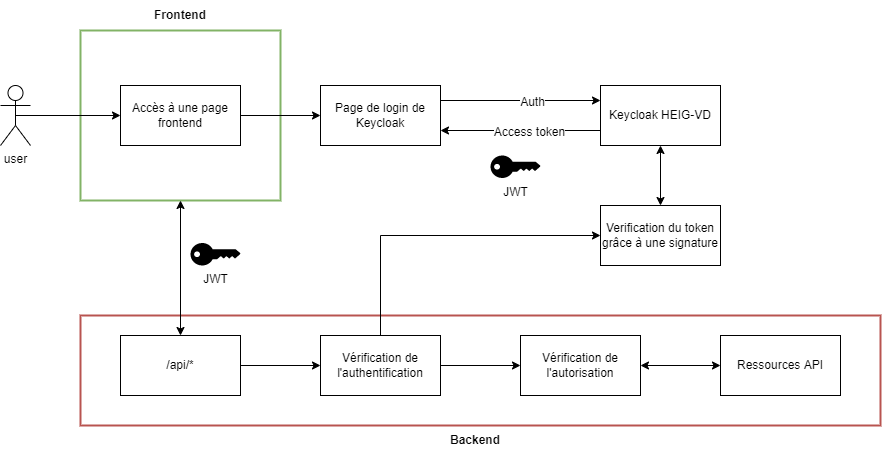
\includegraphics[width=\textwidth]{./assets/figures/keycloak-flow.drawio.png}
        \caption{Flow de Keycloak \label{keycloak-flow.drawio}}
    \end{figure}
\end{center}

En consultant la figure \ref{keycloak-flow.drawio} mettant en image notre situation et la figure \ref{keycloak-flow-lib} tirée de la librairie \href{https://github.com/robsontenorio/laravel-keycloak-guard}{laravel-keycloak-guard}, nous comprenons bien que l'utilisateur arrivant sur le site, commence par s'authentifier à l'aide de ses informations d'identification, puis récupère un \Gls{jwt} agissant comme certificat / clé d'accès afin d'effectuer des requêtes au \Gls{backend}. \\
Ce token / jeton est ensuite ajouter dans l'entête de chaque requête vers le \Gls{backend}. \\
Lorsque le \Gls{backend}, reçoit une requête, il vérifie le jeton donné grâce à une signature fournie par le domaine Keycloak de la \Gls{heig-vd} et détermine si ce dernier et valable ou non.

\begin{center}
    \begin{figure}[H]
        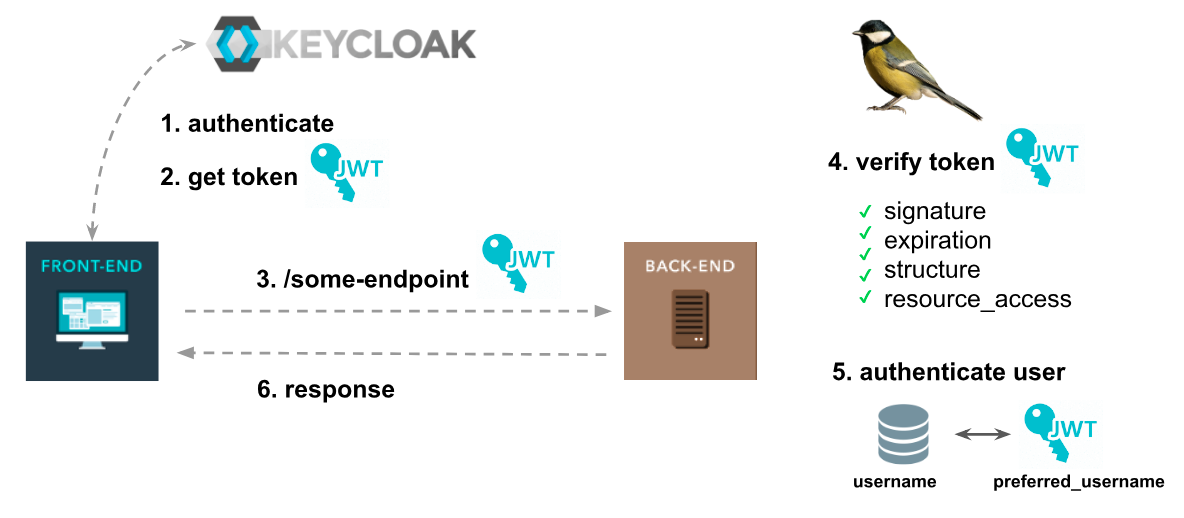
\includegraphics[width=\textwidth]{./assets/figures/keycloak-flow-lib.png}
        \caption{Flow de Keycloak tiré de \label{keycloak-flow-lib}}
    \end{figure}
\end{center}

Le fonctionnement de Keycloak expliqué, il est nécessaire d'expliquer la façon dont il a été implémenté au niveau de \Gls{backend}.

\subsection{Implémentation de Keycloak côté Backend}
Tout d'abord, nous pouvons remarqué sur les figures \ref{routes-api-1} et \ref{routes-api-2}, que l'authentification est utilisée dans le middleware \emph{auth:api}. Ce dernier étant appliqué à toutes les routes de l'\Gls{api}.

Pour ensuite implémenter la logique utilisée par ce middleware, je me suis inspiré d'un packet Laravel existant, \href{https://github.com/robsontenorio/laravel-keycloak-guard}{laravel-keycloak-guard}. Je n'ai pas pu l'utiliser direcement, car il n'était pas totalement adapté à nos besoins.

Pour intégrer mon adaptation de package au projet, j'ai d'abord créer un \emph{KeycloakServiceProvider} comme nous pouvons le voir à la figure \ref{keycloak-service-provider}. \\
Dans ce dernier, nous voyons que nous définissons la \emph{KeycloakGuard} pour l'authentification.

\begin{listing}[H]
    \inputminted{php}{assets/code/KeycloakServiceProvider.php}
    \caption{KeycloakServiceProvider \label{keycloak-service-provider}}
\end{listing}

Ensuite, nous implémentons la \emph{KeycloakGuard} dans un fichier et une classe à part (disponible en annexe). Il est également nécessaire de définir quelques Exception liées à cette implémentation. \\
Tous ces fichiers sont disponibles dans le dossier \emph{/app/Providers/Keycloak}.

De plus, il est nécessaire d'ajouter un fichier de config afin de supporter certains paramètres à fournir dans le \emph{.env} tel que la clé publique permettant de vérifier les tokens. Ce fichier de config doit être créer dans le dossier \emph{config} et se nommer \emph{keycloak.php}. Ce dernier est défini comme sous la figure \ref{keycloak.php}.

\begin{listing}[h]
    \inputminted{php}{assets/code/keycloak.php}
    \caption{auth.php \label{keycloak.php}}
\end{listing}

Finalement, il faut définir la \emph{KeycloakGuard} comme \emph{guard} dans le fichier de configuration \emph{auth.php}, comme montré sur la figure \ref{auth.php}.

\begin{listing}[h]
    \inputminted{php}{assets/code/auth.php}
    \caption{auth.php \label{auth.php}}
\end{listing}

% cliffhanger
Maintenant que le système d'authentification est défini, il est important d'utiliser les personnes authentifiées pour définir les différentes autorisations concernant les ressources de l'\Gls{api} et c'est ce que nous allons voir dans la prochaine section.

\newpage

\section{Autorisation d'accès aux ressources et gestion des droits}

Un système de contrôle d'accès aux ressources basé sur les rôles a été mis en place ou aussi appelé \emph{RBAC (Role Based Access Control)}.
Pour mettre ce système en place, il nous faut des rôles bien défini et c'est ce que nous allons maintenant.

\subsection{Rôles}
Voici les différents rôles:
\begin{itemize}
    \item \emph{admin} représentant un admin de l'application;
    \item \emph{client} représantant un client de l'application (généralement étudiant de la \Gls{heig-vd});
    \item \emph{worker} représantant un technicien;
    \item \emph{validator} représentant un validateur de travail (généralement un professeur).
\end{itemize}

À savoir que le rôle \emph{validator} a été prévu mais non implémenté dans l'application.

Par définition, les rôles worker et validator peuvent être vu comme des sortes d'interface dans le milieu de la programmation.

Nous pouvons donc représenter les rôles sous la forme d'un diagramme, comme la figure \ref{roles-diagram.drawio}

%\figi{roles-diagram.drawio}{16cm}{Diagramme de classe des rôles de l'application}
\begin{center}
    \begin{figure}[H]
        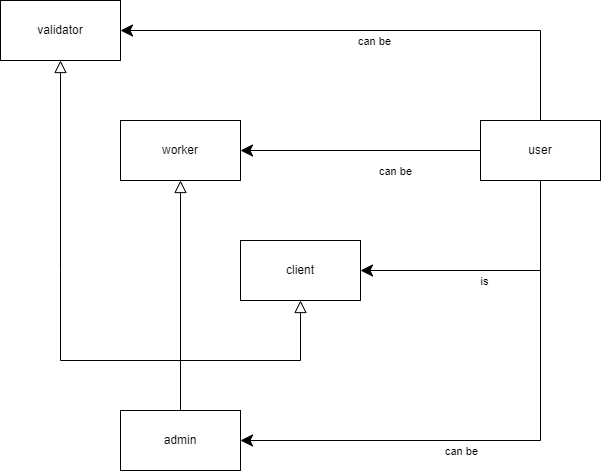
\includegraphics[width=\textwidth]{./assets/figures/roles-diagram.drawio.png}
        \caption{Diagramme de classe des rôles de l'application \label{roles-diagram.drawio}}
    \end{figure}
\end{center}

Quelques précisions s'imposent, nous remarquons que le rôle \emph{client} est donné à n'importe quel utilisateur authentifier par la \Gls{heig-vd}. \\
Nous remarquons aussi que le rôle \emph{admin} possède tous les droits.

Un autre point étant que les utilisateurs anonymes, n'ont accès à aucune ressource fournie par l'\Gls{api}.

Nous allons maintenant voir comment ces rôles sont utilisés pour gérer l'accès aux différentes ressources de l'\Gls{api}.

\subsection{Accès par route et action}
Nous allons maintenant voir par route, quel accès est accordé à quel rôle.
Mais avant cela, un petit rappel sur le nom de fonctions utilisées pour les méthodes \Gls{http} de l'\Gls{api} est nécessaire et est consultable à la figure \ref{rappel-methode-api}.

\begin{table}[h]
    \begin{center}
        \caption{Rappel des méthodes définies par Laravel pour une API \label{rappel-methode-api}}
        \begin{tabularx}{1.0\textwidth} {X|X|X}
            Méthode HTTP & Chemin  & Nom de fonction \\ \hline
            GET          & /       & index           \\
            GET          & /\{id\} & show            \\
            POST         & /       & store           \\
            PUT          & /       & update          \\
            DELETE       & /\{id\} & delete          \\
        \end{tabularx}
    \end{center}
\end{table}

Avant de finalement passer à cette mise en place, une petite légende doit être définie.

\subsubsection{Légende}
Voici un récapitulatif des symboles qui peuvent être utilisés dans les tableaux: \\
x indique que le rôle a accès à la route sans condition.
j / u / m = indique que le rôle a accès à la route sous certaines conditions. Ces conditions seront précisées pour chacune des lettres et des routes.

\subsubsection{Route \emph{files}}
Pour la route \emph{files}, la gestion des autorisations est disponible sur la figure \ref{autorisations-route-files}.

\begin{table}[h]
    \begin{center}
        \caption{Route \emph{files} \label{autorisations-route-files}}
        \begin{tabularx}{1.0\textwidth} {X|X|X|X|X}
            rôles  & show & store & update & delete \\ \hline
            admin  & x    & x     & x      & x      \\
            client & j    & j     & j      & j      \\
            worker & j    &       &        &        \\
        \end{tabularx}
    \end{center}
\end{table}

j = Pour effectuer ces actions, le client / travailleur doit faire partie du travail liée au fichier. \\
Pour les actions du client uniquement, il doit faire partie du travail en tant que client.

\subsubsection{Route \emph{jobs}}

\subsubsubsection{méthodes API}

\begin{table}[h]
    \begin{center}
        \caption{Route \emph{jobs} \label{autorisations-route-jobs}}
        \begin{tabularx}{1.0\textwidth} {X|X|X|X|X|X}
            rôles  & index & show & store & update & delete \\ \hline
            admin  & x     & x    & x     & x      & x      \\
            client &       & j    & x     & j      & j      \\
            worker &       & j    &       &        &        \\
        \end{tabularx}
    \end{center}
\end{table}

j = Pour effectuer ces actions, le client / travailleur doit faire partie du travail. \\
Pour les actions du client uniquement, il doit faire partie du travail en tant que client.

\subsubsubsection{Autres méthodes}

\begin{table}[h]
    \begin{center}
        \caption{Route \emph{jobs} suite \label{autorisations-route-jobs-other-get}}
        \begin{tabularx}{1.0\textwidth} {X|X|X|X|X}
            rôles  & get unassigned jobs & get all user's jobs & get all client's jobs & get all worker's jobs \\ \hline
            admin  & x                   & x                   & x                     & x                     \\
            client &                     & u                   & u                     &                       \\
            worker & x                   & u                   &                       & u                     \\
        \end{tabularx}
    \end{center}
\end{table}

u = Pour effectuer ces actions, le client / travailleur doit être le même utilisateur que celui qui effectue la requête.

\begin{table}[h]
    \begin{center}
        \caption{Route \emph{jobs} suite 2\label{autorisations-route-jobs-updates}}
        \begin{tabularx}{1.0\textwidth} {X|X|X|X|X}
            rôles  & assign a worker & update status & update rating & update notifications \\ \hline
            admin  & x               & x             & x             & x                    \\
            client &                 &               & j             & j u                  \\
            worker & j               & j             &               & j u                  \\
        \end{tabularx}
    \end{center}
\end{table}

j = Pour effectuer ces actions, le client / travailleur doit faire partie du travail. \\
Pour les actions du client uniquement, il doit faire partie du travail en tant que client. \\
Pour les actions du travailleur uniquement, il doit faire partie du travail en tant que travailleur.

u = Pour effectuer ces actions, le client / travailleur doit être le même utilisateur que celui qui effectue la requête.

\subsubsection{Route \emph{messages}}

\begin{table}[h]
    \begin{center}
        \caption{Route \emph{messages} \label{autorisations-route-messages}}
        \begin{tabularx}{1.0\textwidth} {X|X|X|X}
            rôles  & index & show & store \\ \hline
            admin  & x     & x    & x     \\
            client &       & m    & j s   \\
            worker &       & m    & j s   \\
        \end{tabularx}
    \end{center}
\end{table}

m = Pour effectuer ces actions, le client / travailleur doit faire partie du message (en tant qu'expéditeur ou récepteur). \\
j = Pour effectuer ces actions, le client / travailleur doit faire partie du travail liée au message.
s = Pour effectuer ces actions, le client / travailleur doit être l'expéditeur du message.

\subsubsection{Route \emph{users}}

\begin{table}[h]
    \begin{center}
        \caption{Route \emph{users} \label{autorisations-route-users}}
        \begin{tabularx}{1.0\textwidth} {l|l|l|l|l|l|X}
            rôles  & index & show & store & update & delete & update email notifications \\ \hline
            admin  & x     & x    & x     & x      & x      & x                          \\
            client &       & u    &       &        &        & u                          \\
            worker &       & u    &       &        &        & u                          \\
        \end{tabularx}
    \end{center}
\end{table}

u = Pour effectuer ces actions, le client / travailleur doit être le même utilisateur que celui qui effectue la requête.

\subsubsection{Route \emph{job categories}}

\begin{table}[h]
    \begin{center}
        \caption{Route \emph{job categories} \label{autorisations-route-job-categories}}
        \begin{tabularx}{1.0\textwidth} {X|X|X|X|X|X|X}
            rôles  & index & show & store & update & delete & image \\ \hline
            admin  & x     & x    & x     & x      & x      & x     \\
            client & x     & x    &       &        &        & x     \\
            worker & x     & x    &       &        &        & x     \\
        \end{tabularx}
    \end{center}
\end{table}

\subsubsection{Routes admin}
Seul les administrateurs peuvent effectuer des actions sur la route suivante \emph{file\_types}.

\begin{table}[h]
    \begin{center}
        \caption{Routes admin \label{autorisations-route-admin}}
        \begin{tabularx}{1.0\textwidth} {X|X|X|X|X|X}
            rôles  & index & show & store & update & delete \\ \hline
            admin  & x     & x    & x     & x      & x      \\
            client &       &      &       &        &        \\
            worker &       &      &       &        &        \\
        \end{tabularx}
    \end{center}
\end{table}

% cliffhanger
Toute cette conception d'autorisation théorique définie, il est maintenant nécessaire de définir comment elle a été implémentée au niveau du code.

\subsection{Mise en place}
La mise en place du système d'autorisation est basée sur un concepte que \Gls{laravel} fourni, les \href{https://laravel.com/docs/9.x/authorization#creating-policies}{\emph{Policies}}.

Les \emph{Policies} une fois définies, elles sont utilisées et appelées dans un middleware. L'instruction \emph{can} fait appelle au middleware et à la policy correspondante afin de vérifier l'accès à la ressource. Nous voyons bien l'appel à cette fonction dans le fichier \emph{routes/api.php} (\ref{routes-api-1}, \ref{routes-api-2}). \\
Pour chaque route disponible sur une ressource / un modèle, une fonction dans la \emph{Policy} correspondant défini l'accès à cette dernière. \\
Dans chaque \emph{Policy}, il y également une fonction de nommée \emph{before} qui est appelée avant toute vérification. Cette fonction est utilisée afin de vérifier si l'utilisateur possède au moins le rôle \emph{client} ou s'il est \emph{admin}.

La figure \ref{policy-files} est un exemple de \emph{Policy}.

\begin{listing}[H]
    \inputminted{php}{assets/code/FilePolicy.php}
    \caption{Policy de la route \emph{files} \label{policy-files}}
\end{listing}

Il est également nécessaire d'enregistrer chacune des \emph{Policies} dans le tableau \emph{policies} de la classe \emph{AuthServiceProvider}, comme on peut le voir sur la figure \ref{auth-service-provider}.

\begin{listing}[H]
    \inputminted{php}{assets/code/AuthServiceProvider.php}
    \caption{AuthServiceProvider \label{auth-service-provider}}
\end{listing}

% cliffhanger
Il est bien de définir un système de contrôle d'accès aux différentes ressources, mais il est également important de pouvoir retracer ce qu'il s'est passé sur le serveur. C'est ce que nous allons voir grâce à la politique de logging mise en place.

\section{Politique de logging}
Tout d'abord, le logging our journalisation est le fait de tracer l'exécution de certaines actions sur le seveur grâce à des messages stocké dans un fichier de log. \\
C'est un point important du développement d'application informatique car il est légalement demandé de pouvoir retracé certaines requêtes en cas d'enquête. \\
Le logging est également très utile pour le debugging en phase de développement mais également lorsque certains problèmes apparaîssent en production. \\
Le logging contient différent niveau de sévérité, de ce fait une politique de logging doit être définie, afin de savoir quel événement sera assigné à quel sévérité et c'est ce qui a été défini à la figure \ref{politique-log}.

\begin{table}[h]
    \begin{center}
        \caption{Politique de log\label{politique-log}}
        \begin{tabularx}{1.0\textwidth} {l|X}
            Niveau de log & Raison déclanchant le log                                                           \\ \hline
            Emergency     & Pas utilisé                                                                         \\
            Critical      & Pas utilisé                                                                         \\
            Error         & Une erreur interne survient lors d'une requête sur le serveur                       \\
            Warning       & Un utilisateur essaie d'accéder à une ressource ou route dont il n'a pas les droits \\
            Notice        & Pas utilisé                                                                         \\
            Info          & Lorsqu'un utilisateur accède à une route pour laquelle il a des droits              \\
            Info          & Lorsqu'une action de n'importe quel controller est réussie                          \\
            Info          & Lorsqu'une erreur de logique métier se produit                                      \\
            Info          & Lorsqu'il y a un problème avec le fichier téléchargé                                \\
            Debug         & Utilisé pour le debugging                                                           \\
        \end{tabularx}
    \end{center}
\end{table}

\subsection{Niveau de logging du serveur de production}
Un autre point survient lorsque nous souhaitons mettre en place une politique de logging, quel sera le niveau minimum de sévérité utilisé pour la production. En effet, nous ne voulant pas forcément enregistrer la totalité des logs afin de réduire au maximum les fichiers de log et garder les informations essentiels. \\
Dans notre cas, j'ai fixé la limite de sévérité minimum à \emph{Warning} pour la production afin d'obtenir uniquement les informations utiles pour retracer les erreurs de serveur et les tentatives d'accès aux ressources non autorisées. \\
Lors du développement, il est évident que la limite est à \emph{Debug}.

% cliffhanger
Maintenant que nous avons vu qu'il fallait tracer ce qu'il se passe sur le \Gls{backend}, il est important de connaître les messages et status que ce dernier peut nous retourner et c'est ce que nous allons voir dans la section suivante.

\section{Erreurs retrounées par le Backend}
Tout les erreurs retournées par le \Gls{backend} sont des erreurs \Gls{http} et suivent les codes défini par ce protocole. \\
Toutes les erreurs comporte donc un \emph{Status code} et un message / des données. Ces réponses sont toutes transmises au format \Gls{json}. \\
Le tableau \ref{reponses-erreurs-backend} trace les différentes réponses que le \Gls{backend} peut retourner.

\begin{table}[h]
    \begin{center}
        \caption{Réponses et erreurs retournées par le Backend \label{reponses-erreurs-backend}}
        \begin{tabularx}{1.0\textwidth} {l|l|X}
            Status code & Signification         & Événements générant la réponse                                                                   \\ \hline
            200         & Ok                    & L'action a été exécutée avec succès                                                              \\
            400         & Bad Request           & Lorsqu'une erreur de logique métier s'est produite ou que le chemin n'existe pas                 \\
            403         & Forbidden             & L'utilisateur n'a pas le rôle pour utiliser la route sur la ressource                            \\
            404         & Not Found             & Lorsqu'une ressource à laquelle nous essayons d'accéder n'est pas trouvée ou n'existe pas        \\
            422         & Unprocessable Entity  & Lorsqu'une erreur se produit à cause d'une entrée utilisateur incorrecte                         \\
            500         & Internal Server Error & Lorsqu'une erreur que le serveur ne peut pas gérer est survenue pendant l'exécution d'une action \\
        \end{tabularx}
    \end{center}
\end{table}

% cliffhanger
Maintenant que nous avons vu toutes les réponses que le \Gls{backend} peut fournir et qu'il peut parfois renvoyé une erreur liée à une mauvaise entrée utilisateur, nous allons voir comment valider ces entrées utilisateurs et comment sont renvoyées ces erreurs dans la prochaine section.

\section{Validation des entrées utilisateurs}
Pour commencer les entrées utilisateurs peuvent être contenu à 2 endroits lors d'une requête. Elles peuvent être dans la \emph{query string} ou dans le \emph{body} de la requête HTTP.

\subsection{Query string}
Pour valider les entrées utilisateurs dans les query string, il est possible de définir des \Gls{regex} pour tous les paramètres portant le même nom des fichiers du dossier \emph{routes}.
Pour cela, il faut modifier le fichier \emph{RouteServiceProvider} comme indiqué sur la figure \ref{route-service-provider} afin d'ajouter toutes les entrées que nous souhaitons valider.

\begin{listing}[h]
    \inputminted{php}{assets/code/RouteServiceProvider.php}
    \caption{RouteServiceProvider \label{route-service-provider}}
\end{listing}

\subsection{Form Request}
Pour valider les entrées utilisateurs dans le corps de la requête, un architecture de code plus compliquée doit être mise en place. \Gls{laravel} fournit la possibilité de valider les requêtes grâce à des \href{https://laravel.com/docs/9.x/validation#form-request-validation}{\emph{Form Request}} et c'est ce que j'ai utilisé. \\
Le but de ces \emph{Form Request} étant de définir une liste de règles précises pour un type de requête précis, par exemple, insérer un nouveau \emph{job}. Ces règles vont valider les entrées utilisateurs et vont ensuite nous permettre d'être sûr de travailler avec des données valides.

Toutes les \emph{Form Request} sont disponibles dans le dossier \emph{/app/Http/Requests}. \\
Sur la figure \ref{job-category-request}, nous pouvons observer un exemple de tableau de règles définies pour l'insertion ou la mise à jour d'une catégorie de travail. \\
À savoir que toutes les règles utilisables sont disponibles sur la doc \href{https://laravel.com/docs/9.x/validation#available-validation-rules}{Laravel}

\begin{listing}[H]
    \inputminted{php}{assets/code/JobCategoryRequest.php}
    \caption{JobCategoryRequest \label{job-category-request}}
\end{listing}

\newpage

\subsection{Regex}
Comme vous l'avez peut-être remarqué sur la figure \ref{job-category-request}, il y a également des règles impliquant des \Gls{regex} et ces dernières sont définies ailleurs dans le code. \\
Ces \Gls{regex} se trouvent dans la classe disponible en suivant le chemin \emph{/app/Constants/Regex.php}. Toutes ces \Gls{regex} ont été mise en place afin de valider le maximum d'entrées utilisateurs du programme et utilisées dans les \emph{Form Request}.

\subsection{Constantes}
Je tiens à préciser que toutes les classes contenant des constantes utilisées dans l'application sont disponibles dans le dossier \emph{/app/Constants}.

% cliffhanger
Maintenant que nous avons vu comment valider les entrées utilisateurs, nous allons nous intéresser à des entrées utilisateurs un peu moins classique, les fichiers. Comment réussir à gérer la validation, l'upload et le download de fichiers pour l \Gls{backend}, C'est ce que nous allons voir dans la prochaine section.

\section{Gestion des fichiers}
Tout d'abord, il faut savoir que toute la gestion des fichiers est réalisée dans le modèle \emph{File}, toute cette partie peut-être définie comme un \emph{File Service}.

\subsection{Validation de fichiers}

Pour commencer avec la réalisation de ce \emph{service}, nous allons parcourir la validation de fichier. \\
Il faut savoir que \Gls{laravel} fournit la possibilité de récupérer des informations sur le fichier qui est en train d'être upload, ces dernières peuvent être consultée en suivant le lien suivant: \href{https://laravel.com/docs/9.x/filesystem#other-uploaded-file-information}. \\

Pour valider un fichier, certains conditions doivent être respectées, les voici:
\begin{itemize}
    \item le fichier ne doit pas être \emph{null};
    \item le fichier ne doit pas dépasser la taille de 10 Mo;
    \item le fichier doit avoir une extension qui correspond au type de fichier détecté en l'inspectant;
    \item le fichier doit posséder un type contenu dans la base de données;
    \item le fichier doit posséder un type accepter par la catégorie de travail auquel le job est relié.
\end{itemize}

Toutes ces validations sont réalisées dans une fonction nommée \emph{is\_valid\_file} que vous pouvez consulter à la figure \ref{file-validation}. Cette fonction est utilisée dans toutes les \emph{Form Request} nécessitant un fichier.

\begin{listing}[H]
    \inputminted{php}{assets/code/FileValidation.php}
    \caption{fonction is\_valid\_file du \emph{File Service} \label{file-validation}}
\end{listing}

Un point important concernant la validation de fichier étant le type de fichier qui est détecté par la fonction \emph{extension} de Laravel. Cette dernière inspecte le fichier et détermine son type. Cette dernière fonctionne très bien avec les types de fichiers classique, cependant, certains types de fichiers qui m'ont été demandé d'ajouter, ne sont pas du tout détecté correctement par cette dernière. \\
De ce fait, j'ai dû trouvé une solution et la voici. J'ai créé deux listes constantes de types de fichiers non supportés par cette fonction. \\
La première liste défini les types de fichiers dont j'ai pu testé l'upload et donc obtenir le type retourné par la fonction \emph{extension}. Cette liste fait également l'objet d'un tableau de correspondance qui est utilisé lorsqu'il faut vérifier le type du fichier. \\
La seconde liste contient tous les types de fichiers que je n'ai pas pu tester et qui esquiveront donc la vérification de la fonction \emph{extension}. \\
Une façon d'améliorer cette solution un peu "bout de bois" serait d'essayer d'utiliser la fonction \emph{mime\_content\_type} de \Gls{php}.

Une autre requête m'a été demandée en fin de projet, les types de fichiers compressé devraient si possible être validé en observant également les fichiers à l'intérieur du fichier compresser et en les validant. Cette demande n'a pas pu être mise en place pour le moment, mais des essaies ont été tentés et sont disponibles en commentaires dans le code principal, ainsi que sur l'issue ouverte sur \Gls{github}.

% cliffhanger
Une fois les fichiers validés, il faut les upload, mais où? C'est ce que nous allons voir maintenant.

\subsection{File Storage}
Pour stocker des fichiers, \Gls{laravel} propose un système de \href{https://laravel.com/docs/9.x/filesystem}{\emph{File Storage}}. Pour ce projet, il a été décidé d'utiliser un stockage de fichier local. Au niveau local, 2 \emph{disques} sont disponibles, le \emph{public} et le \emph{private}. \\
Le premier ayant pour but d'exposer des fichiers que tout le monde peut consulter et le second de conserver des fichiers afin de définir plus tard qui pourra les consulter. \\

Dans notre projet, nous utilisons le disque \emph{public} afin de stocker les images des catégories de travaux sous le dossier \emph{images} et le disque \emph{private} pour stocker tous les autres fichiers upload par les utilisateurs.

Ces disques sont disponibles au chemin \emph{/storage/app}.

% cliffhanger
Maintenant que nous savons où stocker ces fichiers, regardons comment les upload.

\subsection{Upload de fichiers}
Un des points les plus importants pour upload des fichiers, est le faite que nous souhaitons éviter de stocker 2 fois le même fichier et cela pour conserver le maximum de mémoire possible. Pour ceci, nous allons commencer par \Gls{hash} le contenu du fichier et récuper ce dernier afin de le stocker sous le nom du \Gls{hash}. \\
Nous allons ensuite créer un dossier par fichier avec uniquement les 2 premières lettres du \Gls{hash}. Cette petite manipulation est nécessaire pour éviter d'arriver à la limite de stockage par dossier de \Gls{laravel}. \\
De plus, il est nécessaire de une entrée dans la base de données avec toutes ces informations afin de pouvoir retrouver le fichier plus tard. \\
Nous générons un événement, nous verrons à quoi il sert plus tard. \\
Finalement, nous stockons le fichier sous le bon disque et le bon dossier.

Toute cette procédure est disponible en code sous la figure \ref{file-upload}.

\begin{listing}[H]
    \inputminted{php}{assets/code/FileUpload.php}
    \caption{fonction \emph{store\_file} du \emph{File Service} \label{file-upload}}
\end{listing}

De la même façon, avec le \Gls{hash} et la parade des dossiers, le \emph{File Service} gère également la mise à jour et la suppression d'un fichier.

% cliffhanger
Upload des fichiers c'est bien, mais pouvoir les récupérer et les utiliser, c'est encore mieux!
C'est ce que nous allons voir maintenant.

\subsection{Download de fichiers}
Pour récupérer des fichiers, 2 façons sont disponibles, soit nous for4ons l'utilisateur à télécharger un fichier, soit nous créons un \Gls{url} sur le disque \emph{public} où nous pouvons consulter le fichier. \\
Ces deux méthodes ont été mise en place, la première est utilisée pour télécharger les fichiers ajoutés par les utilisateurs, tandis que la seconde est utilisé pour afficher les différentes catégories de travail au niveau du \Gls{frontend}. \\
Le code permettant de réaliser ces deux actions est disponible sur la figure \ref{file-download}.

\begin{listing}[H]
    \inputminted{php}{assets/code/FileDownload.php}
    \caption{Fonctions download\_file et get\_file\_url du \emph{File Service} \label{file-download}}
\end{listing}

Le codee utilise les fonctions fournies par \Gls{laravel} consultable sur la \href{https://laravel.com/docs/9.x/filesystem#downloading-files}{documentation pour le download} et la \href{https://laravel.com/docs/9.x/filesystem#file-urls}{documentation pour les urls}.

% cliffhanger
Maintenant que nous en avons terminé avec la gestion des fichiers, il est nécessaire de parler des événements retraçant tout ce qui s'est passé dans l'application et c'est ce que nous allons faire dans la prochaine section.

\section{Gestion des événements et notifications}
Pour notre application, nous souhaitons réaliser une timeline indiquant tous les événements intervenu sur le travail consulter afin d'avoir un suivi total. Pour réaliser cette timeline, la mise en place d'événements a été conçue. Nous avons déjà vu plus tôt ce que contenait un événement dans la base de données, il est maintenant nécessaire de définir quand est-ce qu'un événement est créé et pourquoi. La figure \ref{events-email-scenario.drawio} défini parfaitement dans quelle situation un événement est généré. \\
À gauche nous observons la personne réalisant l'action indiquée, puis à droite l'événement généré et la personne qu'il doit notifier. \\
Nous pouvons clairement comprendre quel type d'événement est généré dans quelle situation. \\
Il est important de prendre en compte que lorsqu'un événement est créé dans chacune des ces actions, ce dernier a forcément la valeur \emph{to notify} à \emph{true} et va donc indiquer à l'utilisateur concerné (à droite) la notification sur le travail lié.

%\figi{events-email-scenario.drawio}{16cm}{Conception des événements pour les notifications et la timeline}
\begin{center}
    \begin{figure}[H]
        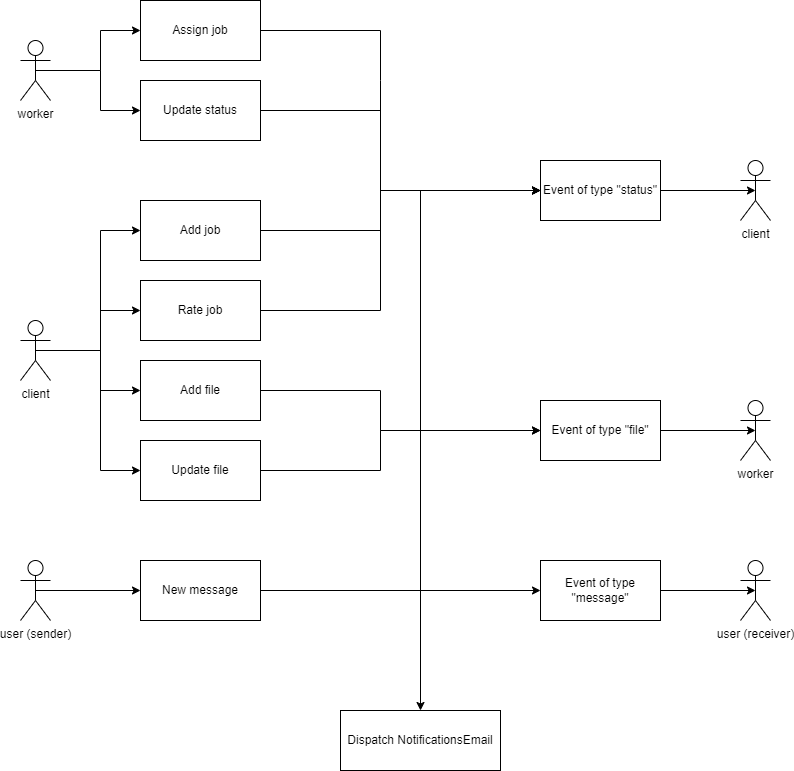
\includegraphics[width=\textwidth]{./assets/figures/events-email-scenario.drawio.png}
        \caption{Conception des événements pour les notifications et la timeline \label{events-email-scenario.drawio}}
    \end{figure}
\end{center}

% cliffhanger
Nous pouvons également voir que quand un événement est généré, un email est préparé et c'est ce dont nous allons parler dans la prochaine section.

\section{Envoi d'email}
L'envoi d'email a été réalisée en suivant la \href{https://laravel.com/docs/9.x/mail}{documentation \Gls{laravel} à ce sujet}. \\
Comme les emails ne doivent pas être envoyé tout de suite mais uniquement après 10 minutes, la mise en place d'un \href{https://laravel.com/docs/9.x/queues#creating-jobs}{\emph{Job}} et d'une \emph{Queue} a également été nécessaire. \\
Au final, ce n'est pas le mail qui est retardé, mais le \emph{Job} qui envoie le mail qui l'est.

Les \emph{Jobs} en attente sont stockés dans la base de données en attendant d'être exécuter. \\
De ce fait, deux tables ont été ajoutées aux \emph{migrations}, ce sont les tables \emph{jobs\_queue} et \emph{failed\_jobs}.

Pour mettre en place notre système de mail et de queue, un \emph{NotificationsEmailJob} a été créé, disponible dans le dossier \emph{/app/Jobs} ainsi qu'un \emph{NotificationsEmail} disponibles dans le dossier \emph{/app/Mail}. \\
Une méthode permettant de \emph{dispatch} le \emph{NotificationsEmailJob} a été ajouté au modèle \emph{Event} comme méthode de \emph{service}. Cette dernière \emph{dispatch} simplement le mail en fonction du statut de l'environnement (production ou développement). \\
La fonction a appelé est la suivante:
\begin{lstlisting}
    NotificationsEmailJob::dispatch($id)->delay(now()->addMinutes(10));
\end{lstlisting}

Cela a pour effet de stocker l'\emph{Event} dans la base de données comme expliqué précédement et il sera automatiquement exécuter après le temps indiqué lors de l'appel de la fonction.

Pour vous expliquer comment le système de mail fonctionne en adéquation avec les événements générés pour la timeline et les notifications, un diagramme de séquence est à disposition sur la figure \ref{events-email-sequence}.

\begin{center}
    \begin{figure}[H]
        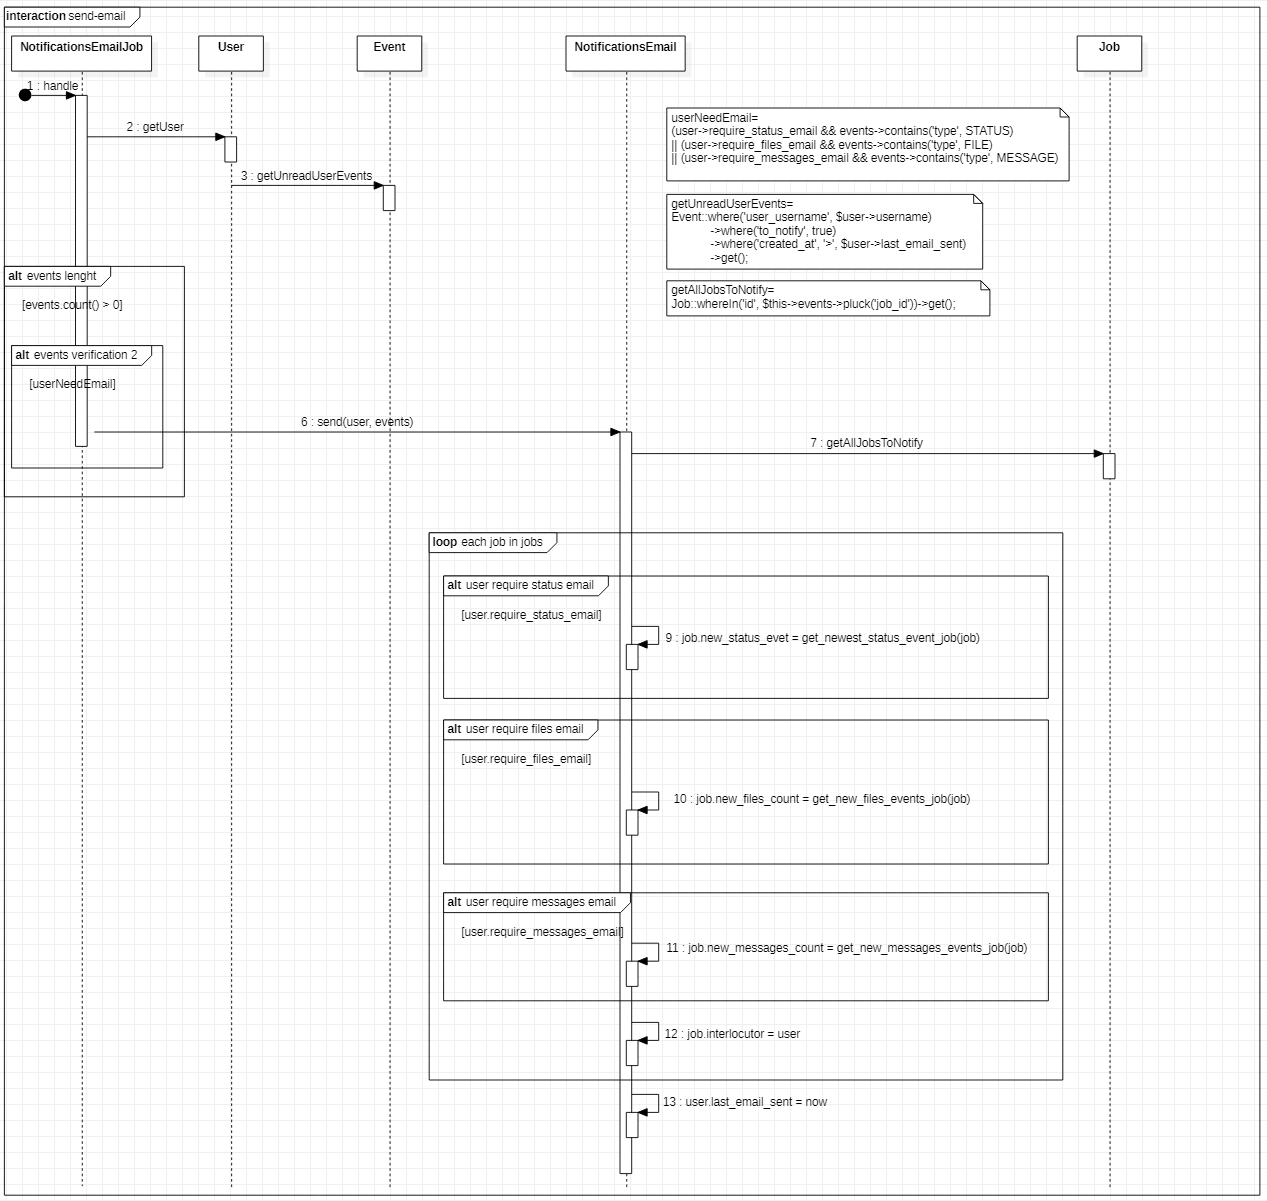
\includegraphics[width=\textwidth]{./assets/figures/emails-events-sequence.png}
        \caption{Diagramme de séquence pour la génération d'un email \label{events-email-sequence}}
    \end{figure}
\end{center}

Le but principal de ce schéma est de montrer que seuls les événements de l'application sont utilisés pour déterminer si un email doit être envoyé à l'utilisateur ou non.

En plus de tout ceci, il est également nécessaire de configurer le fichier de config \emph{mail.php} afin que nous puissions utiliser le service mail de la \Gls{heig-vd} en production. Cette configuration est disponible sur la figure \ref{config-mail}.

\begin{listing}[H]
    \inputminted{php}{assets/code/mail.php}
    \caption{Configuration ajoutée au fichier mail.php \label{config-mail}}
\end{listing}

Dernier point sur ce sujet, la classe \emph{NotificationsEmail} créé un email en utilisant une vue réalisée grâce à \href{https://laravel.com/docs/9.x/blade}{\Gls{laravel} Blade} et disponible sous \emph{/resources/views/mails/email.blade}.

% cliffhanger
Maintenant, que nous avons vu comment mettre en place des emails, nous allons passé au dernier point spécifique de cette application, les \Gls{websockets}.

\section{Websockets}
Pour que notre application soit réactive, dans le sens où un utilisateur n'ait pas besoin de raffraichir la page afin de voir apparaître les changements qu'une autre personne aurait pu apporter sur une donnée observée, le choix des webosckets avait été réalisé. \\
Une solution classique pour contrer le problème énoncer, est d'utiliser un service externe, comme \href{https://pusher.com/}{\emph{pusher}} recevant les changements du bakcend et les propageants au \Gls{frontend} via des canaux. \\
Le système utiliser est basé sur le même principe, mais au lieu d'utiliser directement \emph{pusher}, la librairie permet de lancer un serveur \Gls{websockets} imitant celui de pusher et donc d'éviter de passer par un service externe non maîtriser et potentiellement payant. \\
Cette librairie est nommée \href{https://beyondco.de/docs/laravel-websockets/getting-started/introduction}{\emph{Laravel Websockets}}. Un guide de mise en place est disponible et c'est celui que j'ai suivi.

\subsection{Events}

Pour mettre en place ce système de Webosckets, j'ai d'abord défini tous les événements (\emph{Events}) qui pouvait intervenir et être utiliser par les Webosckets. Je me suis inspiré de \href{https://laravel.com/docs/9.x/events}{la documentation Laravel sur les \emph{Events}} pour les créer et réaliser.
Ces "scénarii" sont disponibles sur la figure \ref{ws-conception-notifications.drawio}. \\
Nous remarquons à gauche l'\emph{Event} qui peut-être généré et à droite le canal dans lequel il sera transmis puis quel type d'utilisateur le recevra. \\
Un Event est au final un objet contenant le canal sur lequel il doit être envoyé et les données qu'il doit envoyer.

%\figi{ws-conception-notifications.drawio}{16cm}{Conception des événements pour les Websockets}
\begin{center}
    \begin{figure}[H]
        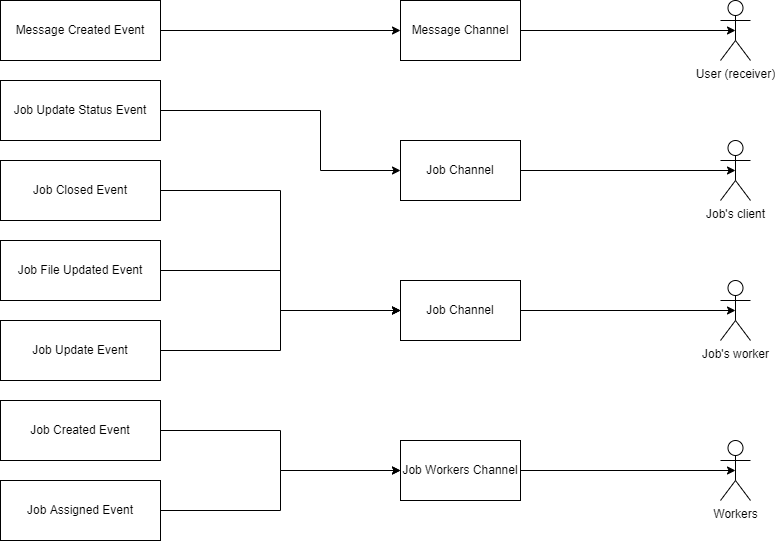
\includegraphics[width=\textwidth]{./assets/figures/ws-conception-notifications.drawio.png}
        \caption{Conception des événements pour les Websockets \label{ws-conception-notifications.drawio}}
    \end{figure}
\end{center}

Un exemple de code d'un \emph{Event} est disponible à la figure \ref{event-exemple}. \\
Comme expliqué précédemment, nous remarquons la méthode \emph{broadcastOn} retournant le channel sur lequel doit être transmis les données lorsque cet événement intervient. \\
Nous pouvons également remarquer l'utilisation de l'interface \emph{ShouldBroadcastNow} permettant d'émettre la diffusion de l' \emph{Event} de façon synchrone.

\begin{listing}[H]
    \inputminted{php}{assets/code/JobAssignedEvent.php}
    \caption{Exemple d'un \emph{Event} avec le \emph{JobAssignedEvent} \label{event-exemple}}
\end{listing}

Il a ensuite fallu configurer ces différents channels comme utilisé sur la figure précédente \ref{event-exemple}. Ces définitions de channels sont réalisées dans le fichier \emph{/routes/channels.php} que nous pouvons consulter sur la figure \ref{ws-channels}. \\
Dans ce fichier, les channels défini possède une fonction qui détermine si l'utilisateur le droit ou non de se connecter au channel.

\subsection{Channels}

\begin{listing}[H]
    \inputminted{php}{assets/code/channels.php}
    \caption{Channels pour le Broadcast sur les Websockets \label{ws-channels}}
\end{listing}

Un \emph{Event} peut ensuite être envoyer / \Gls{broadcast} grâce à l'instruction suivante:
\begin{lstlisting}
    broadcast(new JobClosedEvent($job));
\end{lstlisting}


\subsection{Fichiers de configuration}
Finalement, il est nécessaire de configurer les fichiers de config liés au \Gls{broadcast} et aux \Gls{websockets}, ces derniers se trouvent dans le dossier \emph{/config}. \\
Le premier fichier à configurer est nommé \emph{broadcasting.php} est se voit ajouter la configuration disponible sur la figure \ref{ws-broadcasting}. \\
Il est important de remarquer que le maximum de données sont associées aux valeurs données dans le \emph{.env} afin d'éviter de changer le code entre la phase de développement et la release pour que cela soit adapté à la production. \\
Cette manière de faire permet d'avoir un fichier \emph{.env} pour le développement et un fichier \emph{.env} pour la production et donc ne jamais toucher / changer le code pour faire fonctionner l'un ou l'autre.

\begin{listing}[H]
    \inputminted{php}{assets/code/broadcasting.php}
    \caption{Fichier de configuration pour le broadcasting \label{ws-broadcasting}}
\end{listing}

Le second fichier à configurer est nommé \emph{webosckets.php} est se voit ajouter la configuration disponible sur la figure \ref{ws-broadcasting}. \\
Comme pour le premier fichier et pour les mêmes raisons, un maximum de données sont associées aux valeurs données dans le \emph{.env}. \\
Nous pouvons remarquer les lignes \emph{verify\_peer} et \emph{verify\_peer\_name} qui sont à false afin d'accepter les certificats autosignés.

\begin{listing}[H]
    \inputminted{php}{assets/code/websockets.php}
    \caption{Fichier de configuration pour les Websockets \label{ws-websockets}}
\end{listing}

Un point important qui sera discuté plus tard dans le rapport, est que je n'ai malheureusement pas réussi à faire fonctionner la configuration en production. \\
Au niveau local, le  \Gls{backend} semble bien réussir à se connecter au webosckets et y propager des \emph{Events}, cependant le \Gls{frontend} ne semble pas les recevoir. \\
J'ai pu vérifier ceci grâce à la console mise à disposition par la librairie et accessible au chemin \emph{/laravel-websockets}, ainsi qu'avec des console.log du côté \Gls{frontend}.

% cliffhanger
Et pour couronner le tout, nous devons aborder l'\Gls{api} accessible uniquement par les administrateurs.

\section{API admin}
Cette \Gls{api} réservée aux administrateurs a été ajoutée afin d'améliorer le suivi et faciliter les changements des données sur l'application directement depuis un client \emph{Postman}.
Cette fonctionnalité a été développée afin de maintenir les les ressources / données suivantes:
\begin{itemize}
    \item les utilisateurs (\emph{users});
    \item les catégories de travaux (\emph{job\_categories});
    \item les types de fichiers (\emph{file\_types}).
\end{itemize}

% cliffhanger
Maintenant que nous en avons finalement terminé avec l'implémentation du \Gls{backend}, nous aimerions voir comment l'utiliser via une interface graphique et c'est là qu'intervient le \Gls{frontend}.

\chapter{Conception et Réalisation du Frontend}
Avant de commencer, je tiens à préciser que toute la conception graphique et la réalisation de cette dernière a été réalisée lors du travail de Bachelor de monsieur Lieberherr que vous pouvez retrouver en suivant le lien suivant: \href{https://tb.heig-vd.ch/7532}{Rapport du TB de m. Lieberherr}. \\
Pour rappel, le \Gls{frontend} est un \Gls{spa} (Single Page Application). \\
De ce fait, je ne vais pas documenter toute la conception graphique, je vais me contenter d'expliquer ce que j'ai modifié et ajouté au \Gls{frontend}. \\
Les modifications que j'ai apportées peuvent être séparées dans les thèmes suivants:
\begin{itemize}
    \item mise à jour et nettoyage des dépendances;
    \item ajout de l'authentification avec Keycloak;
    \item adaptation du \Gls{frontend} afin de correspondre à la nouvelle \Gls{api};
    \item ajout des ressources liées aux catégories de travaux;
    \item ajout de la gestion des rôles et modification du \emph{router};
    \item ajout du nombre d'heures de travail réalisées lorsqu'un travail est terminé.
\end{itemize}

\section{Architecture de dossier du projet}
Avant toute chose je tiens à expliquer l'architecture de dossier du \Gls{frontend} qui ne suit peut-être pas totalement les standards ou peut vite changer suivant les développeurs. \\
Voici une liste des dossiers à l'intérieur du dossier \emph{/src} et de leur utilité:
\begin{itemize}
    \item \emph{assets} contient toutes les images, logos, le css et fonts du porjet;
    \item components contient tous les composants que l'application peut utiliser dans les différentes vues;
    \item \emph{constants} contient toutes les fichiers de constantes utilisés dans le code;
    \item containers/navs contient toutes les partie de l'application présentent sur chaque page;
    \item \emph{data} contient toutes les données statiques utilisées dans le code;
    \item \emph{layouts} contient la structure / mise en page de la page de l'application;
    \item \emph{middleware} contient le middleware permettant de mettre à jour le \Gls{jwt};
    \item \emph{plugins} contient le plugin créer pour contenir le code de l'authentification avec Keycloak;
    \item \emph{store} contient tous les fichiers et modules concernant les données stockées dans le \Gls{frontend} et les appels à l'\Gls{api};
    \item \emph{utils} contient un fichier avec des méthodes utilisées par le \Gls{template} de base concernant principalement le menu;
    \item \emph{views} contient toutes les vues de l'application ainsi que les composants liés uniquement à une seul vue.
\end{itemize}

% cliffhanger
Nous allons maintenant parcourir chacune de ces modifications afin de rentrer dans les détails.

\section{Mise à jour et nettoyage des dépendances}
La première chose à noter est la suivante, quand j'ai repris le projet, il y avait plus de 100 dépréciations avec toutes les librairies utilisées. Il faut savoir que le \Gls{frontend} a été réalisé en se basant sur un \Gls{template} acheté et pas forcément très maintenu à jour. \\
Ce \Gls{template} avait le défaut d'utiliser énormément de petites librairies externes ce qui fait vite grossir la liste des dépendances et en avoir trop, ce n'est jamais bon. \\
Heureusement, lorsque monsieur Lieberherr a adapté le \Gls{template} pour réaliser le \Gls{frontend}, il a très peu utiliser les dépendances utilisées par le \Gls{template} original.\\
Après avoir remarqué ce point, j'ai passé passablement de temps à nettoyer les dépendances inutilisées dans le projet et à mettre à jour toutes les dépendances du projet pour finalement arrivé à une liste de dépendances raisonables et qui contient uniquement 21 vulnérabilités.

La majorité de ces vulnérabilités sont liés à la \emph{vue-cli} dont je ne peux pas mettre à jour car tout le projet a été adapté pour avec cette version de \emph{vue-cli}. \\
Le seul moyen de supprimer toutes ces vulnérabilités restantes, serait de repartir d'un projet vierge et ajouté au fur et à mesure les éléments du \Gls{frontend} et à nouveau refaire fonctionner le tout.

Un autre point à noter dans ces dépendances, nous remarquons que plusieurs librairies graphiques offrant souvent les même possibilités sont utilisées. Dans ce genre de cas, il serait préférable d'en choisir une seule. \\
Les librairies sont souvent lourdes en terme de mémoire et en utiliser plusieurs peut donc drastiquement augmenter la taille du site web et de ses pages.

% cliffhanger
Les dépendances mise à jour, il faut maintenant intégrer l'authentification au \Gls{frontend}.

\section{Authentification avec Keycloak}
Pour commencer, je me suis inspiré d'une partie de ce \href{https://davidtruxall.com/secure-a-vue-js-app-with-keycloak/}{tutoriel} afin de mettre en place Keycloak comme un plugin. \\
Le code du \emph{plugin Keycloak} est présent dans le dossier \emph{/src/plugins/} et se nomme \emph{keycloak.js}. \\
L'objectif est principalement de créer un objet \emph{keycloak} global et accessible partout dans le projet afin de pouvoir facilement utiliser le jeton et les informations qu'il possède. \\
La totalité des informations utilisées par le paquet sont enregistrées dans le fichier \emph{.env} du projet afin de protéger les secrets dans le code et adapté au mieux les informations en cas de quelconque changement.

J'ai également créé un middleware nommé \emph{keycloakUpdateToken.js} et se trouvant dans le dossier \emph{/src/middleware} permettant de mettre à jour le \Gls{jwt}. Ce dernier contient la méthode \emph{updateToken} qui va simplement mettre à jour le token en réalisant une requête au serveur d'authentification Keycloak de la \Gls{heig-vd}. \\
Cette méthode est principalement utilisée avant d'envoyer une requête à l'\Gls{api} afin d'être sûr d'avoir un jeton valide comme on peut le voir sur la figure \ref{api-config-js}. \\

\begin{listing}[H]
    \inputminted{js}{assets/code/apiConfig.js}
    \caption{Fichier de configuration pour les appels à l'API \label{api-config-js}}
\end{listing}

Nous pouvons voir que le token est intégrer à chaque entête de requête du \Gls{frontend} à l'\Gls{api} et ceci grâce à la librairie \href{https://axios-http.com/fr/docs/intro}{\emph{axios}} permettant de configurer énormément de paramètres sur les requêtes \Gls{http} et des les envoyer.

Finalement, j'ai intégrer l'objet Keycloak au fichier \emph{main.js} comme montré sur la figure \ref{main-js}.

\begin{listing}[H]
    \inputminted{js}{assets/code/main.js}
    \caption{Fichier principal (main) de Vue.js \label{main-js}}
\end{listing}

% cliffhanger
L'authentification implémentée, nous pouvons maintenant faire des appels à l'\Gls{api} sans soucis. Réaliser des appels à l'\Gls{api} c'est bien, mais utiliser les données récupérées, c'est mieux et c'est ce que nous allons voir maintenant.

\section{Adaptation du Frontend afin de correspondre à la nouvelle API}
Cette section ne sera pas très longue à la différence du temps que j'ai pas passé à adapter le \Gls{frontend}. En effet, la conception du \Gls{backend} ayant drastiquement changé, il a fallu modifier tous les appels à l'\Gls{api} dans le \emph{store}. \\
En parlant de \emph{store} utilisant la librairie \href{https://vuex.vuejs.org/}{\emph{vuex}}, lorsque j'ai récupéré le projet, tout était codé dans le même fichier, ce qui le rendait imbuvable. J'ai donc séparé le \emph{store} en différents modules. Un module par ressource (par exemple les travaux ou messages) a été mis en place. \\
Je me suis inspiré de \href{https://vuex.vuejs.org/guide/modules.html}{la documentation officiel sur les modules} pour intégrer ce concept.

Une fois les appels à l'\Gls{api} réalisés,il a fallu mettre à jour toutes les pages et vues de l'application, et pour réaliser ceci, il n'y a pas de miracle, il faut aller erreur après erreur et bug après bug. \\
Au final chaque page a été adaptée et potentiellement repensée au niveau du code. \\
Les plus gros changements étaient surtout présent au niveau de la gestion des notifications et de la timeline du suivi d'un travail précis. \\
J'ai également remodulé l'architecture de fichiers afin que cela soit plus instinctif.

% cliffhanger
Dans la continuation des adaptations des pages, il a fallu intégrer les catégories de travaux qui auparavant stocké statiquement dans le \Gls{frontend} et nous allons voir maintenant comment elles ont intégrées en provenant du \Gls{backend}.

\section{Ajout des ressources liées aux catégories de travaux}
Le premier ajout a été de rajouter un module dans le \emph{store} dédié aux catégories de travaux et d'y mettre les appels à l'\Gls{api} nécessaires. \\
Ensuite, il a fallu remplacer les informations statiques dans la vue dédiée aux catégories de travaux par celles récupérées de \Gls{api}. \\
Il a également fallu intégrer les images fournies par le \Gls{backend} dans cette même vue.

De plus, il a fallu intégrer dans le reste des pages afin que ces dernières soit utilisées correctement notamment pour:
\begin{itemize}
    \item la création d'un nouveau travail;
    \item les informations sur le travail spécifique;
    \item les tableaux contenant la liste des travaux de l'utilisateur;
    \item les tableaux contenant la liste des travaux non assignés.
\end{itemize}

% cliffhanger
Une fois le \Gls{frontend} totalement adapté, il est nécessaire d'ajouter une gestion des rôles afin de vérifier l'accès à certaines ressources / pages en fonction du rôle de l'utilisateur.

\section{Ajout de la gestion des rôles et modification du \emph{router}}
La première chose que j'ai mise en place est la création d'un fichier de constantes contenant tous les rôles disponibles dans l'application. Ce fichier se trouve dans le dossier \emph{/constants}.

Le routing du \Gls{frontend} a été réalisé avec la librairie \href{https://router.vuejs.org/}{\emph{vue-router}}. Le routing était déjà totalement configuré / réalisé. Les \Gls{url}s de l'application commençaient tous par \emph{/app} et j'ai donc fait en sorte de retirer cet \Gls{url} qui pourrait apparement créer des conflits avec les \Gls{websockets}.

De plus j'ai changé le nom de certaines routes afin qu'elles soient plus instinctives. Le fichier contenant toute la gestion de routes est nommé \emph{router.js} et est consultable sur la figure \ref{router-js}.

\begin{listing}[h]
    \inputminted{javascript}{assets/code/router.js}
    \caption{Router de l'application Vue.js \label{router-js}}
\end{listing}

Pour finir, j'ai ajouté une garde devant la seule route demandant d'avoir un autre rôle que \emph{client}. La route est celle des travaux non assignés \emph{/unassigned-jobs}. \\
Pour accéder à cette dernière, il faut que l'utilisateur stocké dans le \emph{store} possède le rôle \emph{worker} ou \emph{admin}.

% cliffhanger
Maintenant que le \Gls{frontend} est opérationnel, il est possible d'ajouter de nouvelles fonctionnalités, et c'est ce que nous allons voir dans la prochaine section.

\section{Ajout du nombre d'heures de travail réalisées lorsqu'un travail est terminé}
La seule fonctionnalité que j'ai ajouté au \Gls{frontend} est la suivante. Lorsque un travail indique qu'une tâche est terminée, il lui est demandé d'entrer le nombre d'heures passées sur le travail. \\
Pour ajouter cette fonctionnalité, j'ai observé la mise à jour du statut et quand ce dernier était sélectionner à \emph{Terminé}, un champ numérique s'ajoute afin de demander le nombre d'heures passées sur le travail. Nous pouvons voir le résultat final sur la figure \ref{nb-worked-hours}.

\begin{center}
    \begin{figure}[H]
        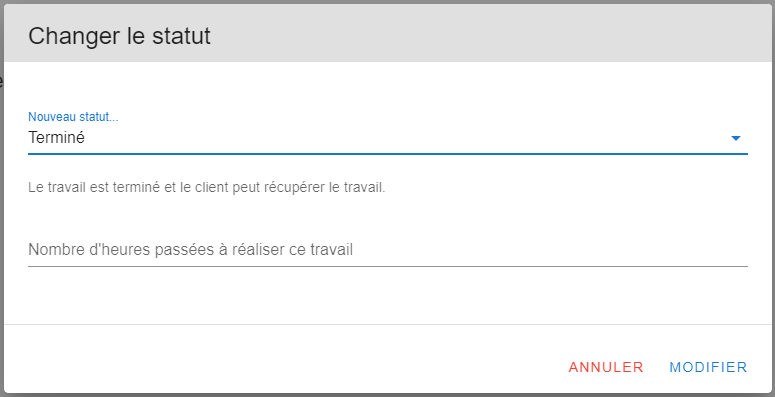
\includegraphics[width=\textwidth]{./assets/figures/nb-worked-hours.png}
        \caption{Interface pour entrer le nombre d'heures passées sur un travail \label{nb-worked-hours}}
    \end{figure}
\end{center}

% cliffhanger
Maintenant que nous en avons finalement terminé avec l'implémentation du \Gls{backend} et du \Gls{frontend}, nous aimerions savoir comment tester l'application et être certain de son bon fonctionnement et c'est exactement ce que nous allons voir au prochain chapitre.

\chapter{Intégration continue et tests}
Avant de parler d'intégration continue, parlons de tests.

\section{Tests}
Dans ce chapitre, nous allons nous concentrer sur les tests réalisés et prévus pour l'application. \\
Le premier point important étant que seul des tests automatisés ont été prévus pour le \Gls{backend}. Il a été estimé que des tests automatisés sur la partie graphique du \Gls{frontend} prendrai trop de temps et ne serait pas rentable car le \Gls{frontend} peut changer rapidement et demanderai beaucoup de temps pour également adapter les tests. \\
Cependant, des tests du système global ont été rédigés, comme nous le verrons plus tard.

\subsection{Tests automatiques}

Les tests automatiques réalisés peuvent être séparés en deux types:
\begin{itemize}
    \item les tests unitaires;
    \item les tests d'intégration.
\end{itemize}

\subsubsection{Tests unitaires}
Les tests unitaires ont été uniquement réalisé sur les \Gls{regex}, ces derniers permettant de valider le bon fonctionnement de la validation d'entrée utilisateurs.

Nous pouvons retrouver ces tests dans le dossier \emph{/tests/Unit}.

\subsubsection{Tests d'intégration}
Les tests d'intégration ont été réalisés sur toutes les routes majoritairement utilisées par les utilisateurs. Ces tests sont des tests dit \emph{end-to-end} et ont été réalisés en suivant \href{https://laravel.com/docs/9.x/http-tests}{la documentation \Gls{laravel} à ce sujet}.

Des tests sur la validation de fichiers upload ont également été réalisés.

Nous pouvons retrouver tous ces tests dans le dossier \emph{/tests/Feature}. Chaque dossier contient les tests réalisés sur une ressource / modèle. Chaque fichier représente les tests sur une action / route précise.

\subsection{Protocole de tests}
Comme mentionné précédemment, un protocole de tests a été rédigé. Ce dernier a pour but de tester globalement l'application, que cela soit en production ou en développement. \\
Nous pouvons comparer ce protocole à des tests \emph{système}. \\
Ce dernier est disponible en annexe. \\
Ce protocole est une adaptation de celui réaliser par monsieur Lieberherr.

% cliffhanger
Les tests réalisés, voyons maintenant comment réaliser une \Gls{ci} en les utilisant, dans la suite du chapitre.

\section{CI}

L'intégration continue ou \Gls{ci} a fait l'objet d'un prototype afin de tester le bon fonctionnement
avant de l'intégrer au projet final.\\
Ce prototype a subit plusieurs itérations, il a fallu partir d'une \Gls{ci} simple permettant de juste
exécuter des tests sur un base de données SQLLite sans migration. Puis il a fallu ajouter une base
de données \Gls{mysql} pour reproduire le véritable environnement. Finalement il a fallu intégrer les
migrations et les seeders afin de donner l'opportunité de tester au mieux l'application.\\
Ayant un dépôt Gitub pour le code, la \Gls{ci} a été réalisée avec \Gls{github} Actions.\\
La \Gls{ci} est consultable sur les figures \ref{ci-1} et \ref{ci-2}

\begin{listing}[h]
    \inputminted{yaml}{assets/code/ci-1.yml}
    \caption{CI pour Laravel \label{ci-1}}
\end{listing}

\begin{listing}[h]
    \inputminted{yaml}{assets/code/ci-2.yml}
    \caption{CI pour Laravel \label{ci-2}}
\end{listing}

\subsection{Déclenchement de la CI}
La première partie après le mot clé \emph{on}, indique quand cette \Gls{ci} et donc cette \Gls{github} Actions est déclanchée.

\subsection{Infrastructure et services}
Ensuite, il est nécessaire d'indiquer sur quel type de machine on souhaite faire tourner notre
installation et nos tests. Il faut également construire les services nécessaires au bon
fonctionnement des tests. Ici nous construisons un \Gls{sgbd} \Gls{mysql}, ainsi qu'une base de données.

\subsection{Étapes de configuration}

À partir du mot clé \emph{steps}, une série d'étape de configuration a lieu. \\
Chaque étape est décrite après le mot clé \emph{name}\\
Tout d'abord, nous lançons les \Gls{github} Actions, puis nous réalisons une étape non obligatoire mais
importante, nous vérifions si la connexion à \Gls{mysql} construit plus tôt fonctionne.\\
Il est notamment important d'installer tout l'environnement \Gls{php}.\\
Il faut ensuite générer les clés pour l'appluication, puis lancer les migrations et le
seeding.\\
Il est ensuite important de changer les permissions pour le storage. Et finalement il est possible
de lancer tous les tests de l'application avec \emph{phpunit}. \\

\section{Code coverage}
Comme vous le remarquez, les tests sont exécutés avec l'option \emph{--coverage clover.xml} afin de générer un rapport de code coverage. \\
Ce rapport de code coverage est stocké dans le fichier \emph{clover.xml}. Ce fichier est ensuite utiliser afin de créer un badge de code coverage au formar \emph{svg} sous le nom \emph{badge-coverage.svg}. \\
Ce badge est présent sur le \emph{README} du dépôt \Gls{github}. \\
Et c'est ainsi que le code coverage a été ajouté au projet.

% cliffhanger
Nous avons une intégration continue mise en place pour réaliser l'application qui est désormais terminée, c'est bien vous me direz, mais nous ne pouvons toujours pas accéder au site, il n'est pas en ligne! \\
Cela tombe bien, nous allons voir dans le prochain chapitre comment déployer l'application web.

\chapter{Déploiement}
Le déploiement, quelle étape importante dans un projet et souvent la plus compliquée.
Je ne vais pas vous mentir, n'étant pas expert dans le domaine, cela n'a pas été facile.

\section{Infrastructure de production}
Avant de commencer à parler du déploiement en lui-même, il est nécessaire de vous présenter l'infrastructure de production mise en place. Cette dernière est visible à la figure \ref{prod-infra}.

\begin{center}
    \begin{figure}[H]
        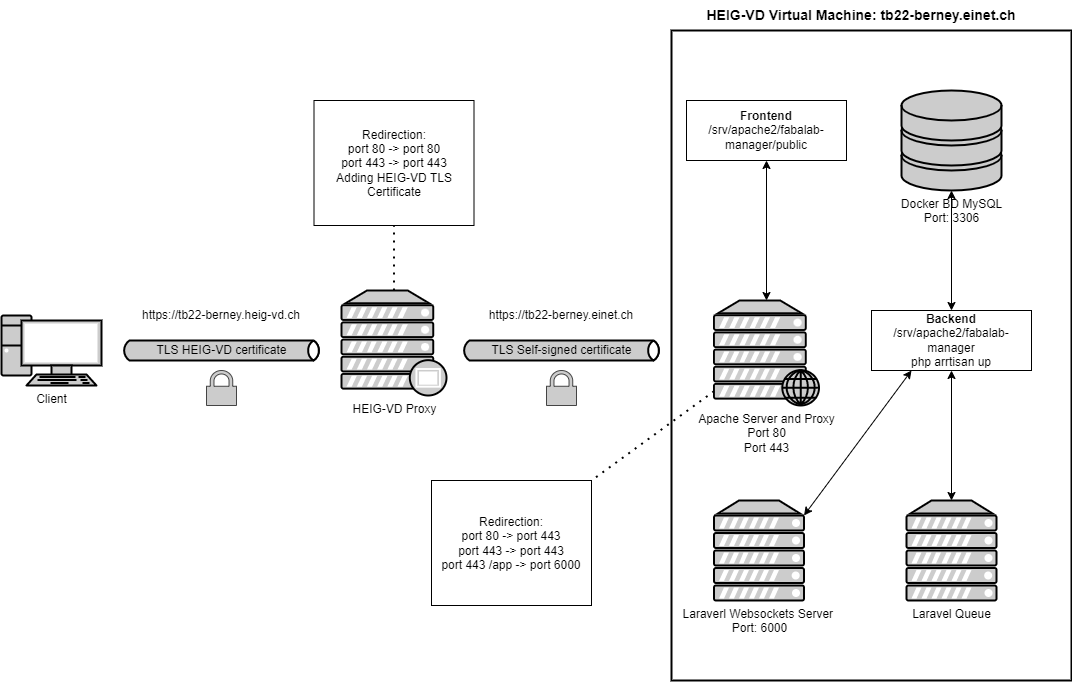
\includegraphics[width=\textwidth]{./assets/figures/prod-infra.png}
        \caption{Infrastructure de production \label{prod-infra}}
    \end{figure}
\end{center}

Tout d'abord, il faut savoir que la machine de production a été fournie par la \Gls{heig-vd}. Cette dernière est donc situé à l'intérieur du réseau de l'école. La machine n'ayant pas d'ouverture directe en \Gls{ssh} ouverte avec l'extérieur, il est obligatoire d'être connecté sur le réseau de l'école physiquement ou via \Gls{vpn}.

Nous pouvons ensuite constater qu'un \Gls{proxy} se situe entre le client et notre serveur. Ce \Gls{proxy} est installé par la \Gls{heig-vd} afin de permettre une entrée sur le serveur via une autre adresse \Gls{dns}, via un autre domaine. d'ouvrir les ports \Gls{http} et \Gls{https}. \\
Ce \Gls{proxy} permet également d'encrypter le flux avec leur propre certificat. Il a pour seul rôle de rediriger le port 443 (\Gls{https}) sur le même port de la machine et pareil pour le port 80 (\Gls{http}). \\
Ces redirections nous force donc à créer un certificat autosigné sur la machine de production afin de pouvoir tout de même accepter les connexions en \Gls{https}.

Nous remarquons également qu'un serveur \Gls{apache} a été mis en place dont nous allons voir la configuration plus tard. Ce dernier sert de serveur \Gls{http} et \Gls{https}. \\
La machine possède également un \Gls{sgbd} tournant sur un container \Gls{docker} à l'aide d'un \emph{Docker-compose}. \\
De plus, il est nécessaire de lancer deux autres services, un pour le serveur \Gls{websockets} et un pour gérer la queue des emails.

\section{Guide d'installation de la machine de production}
Avant de passer aux différentes configurations, il est important de préciser qu'un guide d'installation de la machine de production a été réalisé afin de pouvoir reproduire au mieux l'environnement de travail final. Ce dernier est disponible sur le
\href{https://github.com/heig-fablab/fablab-manager/blob/main/prod-install-guide.md}{dépôt principal sous le nom de \emph{prod-install-guide.md}} et en annexe.

\section{Docker-compose de la BD}
Avant de parler de la configuration \Gls{apache}, il est important de préciser certains points concernant la base de données mise en place. \\
Cette dernière est un \emph{Docker-compose} contenant plusieurs \Gls{conteneur}. Il contient donc le \Gls{sgbd} \Gls{mysql}, hébergement lui-même la base données nommé \emph{fablab-amanager}.

Mais il contient également un \Gls{conteneur} \href{https://www.adminer.org/}{\emph{Adminer}} permettant de gérer la base de données via une petite interface web.

Le dernier \Gls{conteneur} contient un programme permettant de réaliser des sauvegardes des base de données \Gls{mysql} à intervalle régulière et automatiquement, il est nommé \href{https://hub.docker.com/r/databack/mysql-backup}{databack/mysql-backup}.

Toute cette configuration est disponible dans le dossier \href{https://github.com/heig-fablab/fablab-manager/blob/main/mysql/docker-compose.yml}{\emph{mysql} du projet principal} et en annexe.

Nous pouvons maintenant passer à la configuration \Gls{apache}.

\section{Configuration Apache}
Le serveur \Gls{apache} va permettre de servir notre application web. \\
La configuration va simplement pointé sur le dossier \emph{public} du projet \Gls{laravel} et servir les pages web. Ces pages vont communiqué avec le \Gls{backend} lancer en parallèle avec la commande \emph{php artisan up}.

Pour entrer en détail dans la configuration \Gls{apache}, il est important de la vous la présenter avec la figure \ref{config-apache}.

\begin{listing}[H]
    \inputminted{conf}{assets/code/config-apache.conf}
    \caption{Configuration Apache \label{config-apache}}
\end{listing}

Tout d'abord, il faut savoir que la configuration est un \emph{VirtualHost} afin de ne pas toucher aux configurations de base de \Gls{apache}. Cela permet d'avoir plusieurs configuration établies sur le serveur et d'ensuite choisir laquelle est utilisée pour le site.

La configuration réalisée permet de rediriger tout le flux du port 80 sur le port 443 afin de servir le site uniquement en \Gls{https}. Cette redirection peut-être observée au niveau des opérations de type \emph{Rewrite} sous le \emph{VirtualHost *:80}.

Ensuite, nous constatons toutes les informations nécessaire au bon fonctionnement du serveur et indiquant où les pages web à servir se trouvent.

De plus, nous remarquons qu'un \emph{reverse proxy} a été mis en place sur les entrées dédiées aux \Gls{websockets}. Ces derniers passant par le chemin \emph{/app} ou \emph{/apps} sont donc redirigé sur le serveur webosckets tournant sur le port 6000 en local que nous verrons plus tard.

Finalement, nous pouvons observer la configuration permettant de servir le site en  \Gls{https} grâce au certificat autosigné généré avec \href{https://www.openssl.org/}{\emph{OpenSSL}}.

Le serveur \Gls{apache} configuré, nous devons maintenant ajouté les processus supervisés.

\section{Processus supervisé}
Les processus supervisé ont été réalisé avec l'outil \href{http://supervisord.org/}{\emph{Supervisor}}. Cet outil a comme avantage, par rapport au processus \emph{systemctl} classiques de Linux qu'il peut-être intégrer à un \Gls{docker} et offre également une meilleure surveillance des processus.

Pour ajouter des processus gérer par \emph{Supervisor} (une fois installé), il suffit d'ajouter un fichier de configuration par processus sous le dossier \emph{/etc/supervisor/conf.d}. Deux fichiers de configurations ont été créés. \\
Le premier, pour la queue est consulable sur la figure \ref{laravel-queue}.

\begin{listing}[H]
    \inputminted{text}{assets/code/laravel-queue.conf}
    \caption{Configuration pour la queue Laravel \label{laravel-queue}}
\end{listing}

Le second, pour les \Gls{websockets} est consulable sur la figure \ref{laravel-websockets}.

\begin{listing}[H]
    \inputminted{text}{assets/code/laravel-websockets.conf}
    \caption{Configuration pour la queue Laravel \label{laravel-websockets}}
\end{listing}

\emph{Supervisor} permet de toujours maintenir ces processus en vie et de les superviser.

\section{Déploiement continu}
Comme expliqué précédemment, la machine étant uniquement accessible en étant connecté sur le réseau de l'école, il était très compliqué de réaliser un déployement automatique.
De ce fait, un guide de déployement a été réalisé à la place et est disponible en annexe ou à la fin du \href{https://github.com/heig-fablab/fablab-manager/blob/main/README.md}{\emph{REAMDE.md} du dépôt principal}.

L'application web est déployée à l'adresse suivante \href{https://tb22-berney.heig-vd.ch/}{https://tb22-berney.heig-vd.ch/}.

% cliffhanger
Maintenant le site est déployé, prenons du recul sur le projet et établissant un bilan final, passons à la conclusion.

\chapter{Conclusion}

\section{Suite du projet}

\subsection{Récupération des fichiers du projet}
commit du \Gls{frontend} release ws + main -> dans rapport %todo
commit du \Gls{backend} ws + main -> dans rapport %todo
commit du keycloak -> dans rapport %todo

% cliffhanger
Le projet récupéré, regardons ce qu'il reste à corriger et améliorer sur ce dernier.

\subsection{Erreurs restantes}

\subsubsection{Websockets}
Je vais par le plus gros morceau, la mise en place des \Gls{websockets} et de leur serveur.
Comme expliqué dans la partie dédiée de l'implémentation du \Gls{backend}, ces derniers ne fonctionnent pas totalement en local, car le \Gls{frontend} ne reçoit pas les données émisent par le serveur. Cependant le \Gls{backend} arrive bien à les transmettre au serveur hébergeant les \Gls{websockets}. \\
En production, la configuration actuelle ne fonctionne également pas pour le \Gls{backend} qui jette une exception à chaque fois qu'il tente de \Gls{broadcast} un \emph{Event}. Je suis presque sûr que cela est dû à la mauvaise configuration de mon fichier \href{https://github.com/heig-fablab/fablab-manager/blob/main/.env.prod.example}{\emph{.env} de production} disponible en annexe. \\
Le fichier de configuration essaie actuellement de passer par l'\Gls{url} web du serveur, et devrait passer directement en local, ce qui éviterai pas mal de soucis.

En ce qui concerne le \Gls{frontend}, je n'est ai aucune idée d'où vient actuellement le problème comme je ne reçois pas d'erreur, ni de message dans les \emph{logs}.
Je pense aussi que cela vient de ma configuration du fichier \emph{.env}, que cela soit en local ou en production.
Cela pourrait également venir du fait que les \emph{channels} utilisés ne sont pas \emph{public} ou car les instructions de \Gls{broadcast} ne sont pas envoyées avec la fonction \emph{->toOthers()} à la suite de l'instruction \emph{broadcast(new Event(objet))} dans les \emph{Controllers}. \\

Une autre chose dont je suis presque sûr, c'est que la configuration concernant le \emph{reverse proxy} \Gls{apache} doit être fonctionnelle et le problème ne doit pas venir de là.

Selon moi, la procédure pour résoudre le problème est la suivante:
\begin{enumerate}
    \item Faire fonctionner les communications en local en essayant de changer les types de \emph{channels} et / ou la configuration du fichier \emph{.env} et / ou utiliser la fonction \emph{->toOthers()}.
    \item Déployer la version fonctionnelle en locale.
    \item Configurer le fichier \emph{.env} de la production pour faire fonctionner le \Gls{broadcast} du \Gls{backend}.
    \item Configurer le fichier \emph{.env} de la production pour faire fonctionner le \Gls{frontend}.
\end{enumerate}

Pour en finir avec ces \Gls{websockets}, les quatre fichiers d'environnement sont disponibles en annexe et avec les liens suivants:
\begin{itemize}
    \item \href{https://github.com/heig-fablab/fablab-manager/blob/main/.env.prod.example}{\emph{.env.backend.prod}};
    \item \href{https://github.com/heig-fablab/fablab-manager/blob/main/.env.dev.example}{\emph{.env.backend.dev}};
    \item \href{https://github.com/heig-fablab/fablab-manager-frontend/blob/main/.env.prod.example}{\emph{.env.frontend.prod}};
    \item \href{https://github.com/heig-fablab/fablab-manager-frontend/blob/main/.env.dev.example}{\emph{.env.frontend.dev}}.
\end{itemize}

\subsubsection{Queue d'emails en production}
La prochaine erreur restante à aborder est la queue d'emails.
Cette dernière ne semble pas fonctionner parfaitement en production.
En effet, quand je modifie l'entrée \emph{QUEUE\_CONNECTION} avec la valeur \emph{database} dans le fichier \emph{.env} de la production du \Gls{backend}.
Je reçois une exception du \Gls{backend} au moment de stocker le \emph{Job} dans la base de données.
Si cette même entrée contient la valeur \emph{sync}, cela fonctionne mais le \emph{Job} n'attends pas les 10 minutes avant d'être exécuter. \\
Vu l'exception reçue, je pense qu'il y a un problème avec la migration ou le lien entre la fonction \emph{dispatch} et la base de données.

Encore une fois pour résoudre ce problème, il faudrait pouvoir reproduire l'erreur en local, puis la corriger, puis déployer le tout et finalement mettre à jour le fichier \emph{.env} de la production pour que tout fonctionne.

\subsubsection{Conteneur Docker de sauvegarde}
Comme expliqué précédement, un \Gls{conteneur} \Gls{docker} a été ajouté au \emph{Docker-compose} de la base de données afin de faciliter les sauvegardes.\\
La seule chose à dire sur ce point, c'est que je n'ai pas pu tester le bon fonctionnement du \Gls{conteneur} et cela serait à faire.

\subsubsection{Vérification des fichiers compressés}
Comme énoncé dans la partie correspondante, la validation et vérification des fichiers compressées fonctionnent pour le type compressé en lui-même, mais il serait préférable de valider également tous les fichiers à l'intérieur du fichier compresser. \\
Pour cela, j'ai trouvé deux classes \Gls{php} qui peuvent être utilisées afin de récupérer des informations sur les fichiers à l'intérieur du fichier compressé. Ces deux classes sont les suivantes:
\begin{itemize}
    \item \href{https://www.php.net/manual/fr/class.ziparchive.php}{ZipArchive} pour les fichiers \emph{zip};
    \item \href{https://www.php.net/manual/en/class.rararchive.php}{RarArchive} pour les fichiers \emph{rar}.
\end{itemize}

Cependant, aucune classe n'existe pour les fichiers \emph{7z}, il faudrait donc les exclure des types de fichiers accepter.

J'ai également trouvé un \href{https://stackoverflow.com/questions/25847374/ziparchive-check-file-extension}{poste \emph{stackoverflow}} étant très utile pour réaliser ce que nous souhaitons. \\
La fonction \href{https://www.php.net/manual/fr/function.pathinfo.php}{\emph{pathinfo}} pourrait également servir.

Pour finir, tout ce que j'ai déjà exploré est disponible sur \href{https://github.com/heig-fablab/fablab-manager/issues/139}{une \emph{issue} dédiée}.

\subsubsection{Vérification des fichiers avec le mime type de php}
Encore une fois, comme abordé précédemment, les fichiers spéciaux utilisés pour le programme ne sont pas détecté correctement par la fonction \emph{file->extension()} fournie par \Gls{laravel}.
Pour résoudre ce problème, il serait bien de tester la fonction \href{https://www.php.net/manual/fr/function.mime-content-type.php}{\emph{mime\_content\_type} de \Gls{php}} afin d'améliorer drastiquement la qualité et la simplicité du code actuel.

Pour en finir avec ces erreurs restantes, je tiens à préciser que chaque erreur liée au code possède une \emph{issue} ouverte sur le dépôt principal du projet.

\subsection{Améliorations possibles}
voir toutes les issues nice to have

Dans cette section, je vais me contenter de lister des améliorations qui seraient intéressantes à apport au projet en général et qui sont dispensables, nous parlons ici de \emph{nice to have}.

Les améliorations possibles pour le \Gls{frontend} sont donc les suivantes:
\begin{itemize}
    \item \href{https://github.com/heig-fablab/fablab-manager/issues/78}{Réaliser une meilleure gestion des erreurs retournées par le Backend} afin de les afficher / ajouter dans les \emph{toasts} d'erreurs;
    \item \href{https://github.com/heig-fablab/fablab-manager/issues/141}{Améliorer le \emph{design} d'assignation de travaux non attribués} afin de faciliter cette fonctionnalité et limiter le nombre de cliques;
    \item \href{https://github.com/heig-fablab/fablab-manager/issues/156}{Afficher uniquement les types de fichiers accepter} lorsque l'explorateur de fichier est affiché pendant l'ajout de fichiers;
    \item \href{https://github.com/heig-fablab/fablab-manager/issues/122}{Ajouter la possibilité de visualiser des fichiers sur l'application} et cela pour certains types de fichiers;
    \item \href{https://github.com/heig-fablab/fablab-manager/issues/74}{Intégrer tous les messages ou valeurs textuelles en français dans le package \emph{i18n}} afin de pouvoir plus facilement intégrer de nouvelles langues.
\end{itemize}

Les améliorations possibles pour le \Gls{backend} sont donc les suivantes:
\begin{itemize}
    \item \href{https://github.com/heig-fablab/fablab-manager/issues/41}{Ajouter des \Gls{url} pointant sur les routes permettant de les modifier aux données retournées par le \Gls{backend}};
    \item \href{https://github.com/heig-fablab/fablab-manager/issues/100}{Accepter les deux façon de donner l'identifiant d'une donnée dans une route liée à la modification} que ça soit dans la \emph{query string} ou dans le \emph{body} de la requête;
    \item \href{https://github.com/heig-fablab/fablab-manager/issues/22}{Réaliser un \emph{Swagger} pour l'API} et donc \href{https://github.com/heig-fablab/fablab-manager/issues/45}{documenter tout ce dernier avec des \emph{OpenApi tags}};
    \item \href{https://github.com/heig-fablab/fablab-manager/issues/83}{Mieux configurer les paramètres concernant les \emph{CORS}};
    \item \href{https://github.com/heig-fablab/fablab-manager/issues/89}{Intégrer la validation d'un professeur comme étape dans le processus de demande de travail};
    \item \href{https://github.com/heig-fablab/fablab-manager/issues/93}{Tester les \emph{Form Request}} afin de valider totalement les validations d'entrées utilisateurs.
\end{itemize}

Les améliorations possibles pour les \Gls{devops} ou la documentation sont donc les suivantes:
\begin{itemize}
    \item \href{https://github.com/heig-fablab/fablab-manager/issues/126}{Ajouter un badge indiquant que le projet \emph{build}};
    \item \href{https://github.com/heig-fablab/fablab-manager/issues/127}{Ajouter un badge indiquant la licence du projet};
    \item \href{https://github.com/heig-fablab/fablab-manager/issues/134}{Trouver un moyen de faire fonctionner le debugging avec \emph{xdebug}}, ce qui a déjà été testé est disponible sous un fichier \href{https://github.com/heig-fablab/fablab-manager/blob/main/README-coverage-debug-part.md}{README supplémentaire}.
\end{itemize}

\section{Bilan final}
Pour commencer ce bilan final, si nous observons le tableau \ref{taches} contenant toutes les tâches du projet, nous remarquons que j'ai réussi à réaliser toutes les tâches de priorité \emph{Obligatoire} et \emph{Intermédiaire} ou ai trouvé un moyen de les compenser notamment pour la \Gls{cd} automatique. \\
Si l'on parcourt également le cahier des charges défini sur \href{https://gaps.heig-vd.ch/consultation/diplome/affichage.php?id=6135&mode=HTML}{\emph{gaps}}, j'ai également réussi à réaliser tous les points indiqués mis à part les \Gls{websockets} et les envois d'emails différés pour le serveur de production.\\
Je considère également le projet actuellement déployé comme utilisable par le client et c'est un point positif.

Parlant maintenant des regrets que j'ai à propos de ce projet. Le fait que je n'ai pas réussi à faire fonctionner totalement le serveur de production me frustre énormément car j'aurais aimé rendre un travail complet. \\
Cependant cela m'a fait ouvrir les yeux sur des compétences dont je ne possède pas encore et un nouveau monde, une nouvelle dimension de l'éco-système du développement d'application dont je me dois d'explorer et maîtriser à l'avenir. \\
Il est vrai que ma formation n'incluait que très peu de mise en production d'un application et cela ne m'a pas aider pour ce projet, mais je dois être capable d'apprendre ces choses par moi-même. Ce que je n'ai pas pu prendre le temps de faire dans ce projet car le temps ne me le permettait pas vu la charge de travail.

En ce qui concerne toutes les erreurs restantes et pourquoi ces dernières n'ont pas réussi à être réaliser, cela est principalement dû à un projet très conséquent et au manque de compétence dans certains domaines. Certains problèmes sont également apparu très tard dans le projet, à deux semaines de la fin, ce qui laisse très peu de temps sachant qu'il m'a fallu une semaine pour rédiger le rapport final et pauffiner les derniers détails du projet. Je pense aussi que certains problèmes n'étaient pas une priorité au niveau du cahier des charges et ont été mis de côté pour d'autres points plus importants.

Malgrès ces points négatifs, je pense avoir suffisament bien documenté le projet afin qu'il soit repris en main, puis amélioré et terminé.

Pour terminer bilan, je tiens à préciser que je suis tout de même heureux du travail rendu, car tout ce qui est fonctionnel est selon moi bien réaliser. Une petite déception me trotte évidemment dans la tête.

\section{Sources d'informations}
Lors d'un projet de développement informatique, beraucoup de recherches sont réalisées lors de la
phase de développement. Il est impossible de citer toutes les sources utilisées, mais il est
important de citer les forums les plus utilisés, ainsi que les documentations.\\
Voici donc une liste de références:

\begin{enumerate}
    \item laravel.com : documentation de \Gls{laravel} \cite{laravel}.
    \item stackoverflow.com : forum mondial numéro un pour les programmeurs \cite{stackoverflow}.
    \item medium.com : tutoriels divers sur la programmation \cite{medium}.
    \item digitalocean.com : tutoriels, pour \Gls{docker}, \Gls{apache}, Ubuntu et j'en passe \cite{digitalocean}.
    \item keycloak.org: documentation de l'outil d'authentification Keycloak utilisé par la \Gls{heig-vd}.
    \item switch.ch : toute la procédure pour l’utilisation de Shibboleth et Switch edu-id \cite{switch}.
    \item stackshare.io : outil pour comparer des technologies ou utils \cite{stackshare}.
    \item vuejs.org: documentation officiel de Vue \cite{vuejs}.
    \item vuex.vuejs.org: documentation officiel de Vuex \cite{vuex}.
    \item router.vuejs.org: documentation officiel de Router-vue \cite{vue-router}.
    \item beyondco.de : documentation de \Gls{laravel} \Gls{websockets} \cite{beyondco}.
    \item vuetify.com : documentation de la bibliothèque graphique Vuetify \cite{vuetify}.
    \item bootstrap-vue: documentation de la bibliothèque graphique Bootstrap-vue \cite{bootstrap-vue}.
    \item w3schools.com : documentation et exemples pour HTML, CSS et \Gls{javascript} \cite{w3schools}.
    \item wikipedia.org: site d'informations \cite{wikipedia}.
\end{enumerate}

\section{Remerciements}
Dans cette section, je tiens à remcercier toutes les personnes qui m'ont soutenues ou aidé lors de ce projet car sans eux, ils auraient été difficile de mener à bien se projet.

Pour commencer je tiens à remercier monsieur Yves Chevallier pour son suivi sans faille et son implication lors de ce projet. Je le remercie également pour toutes les heures passées avec moi à debugger du \Gls{latex} ou les divers configurations de mon serveur de production.

Je remercie également monsieur Benjamin Wolf pour m'avoir fourni la machine virtuelle de production. Mais également pour m'avoir soutenu dans la mise en place du système d'authentification \emph{Keycloak} de l'école et d'avoir toujours résolu mes quelques soucis lié à la machine de production.

Je remercie aussi mes amis et collègues, Nicolas Crausaz, Maxime Scharwath et Loïc Dessaules pour leurs précieux conseils concernant le \Gls{frontend} et \Gls{apache} pour les deux premiers et le \Gls{backend} pour le dernier.

Finalement, je remercie monsieur Tristant Lieberherr pour avoir passé du temps avec moi en début de projet afin de me mettre sur le droit chemin et m'avoir expliquer ce qu'il a réaliser et tenter de le faire fonctionner sur ma machine.

\vfil
\hspace{8cm}\makeatletter\@author\makeatother\par
\hspace{8cm}\begin{minipage}{5cm}
    %%if
    % Place pour signature numérique
    \printsignature
    %%fi
\end{minipage}
\clearpage

\appendix
\appendixpage
\addappheadtotoc

%%if
\chapter{Plannings}

\begin{landscape}
    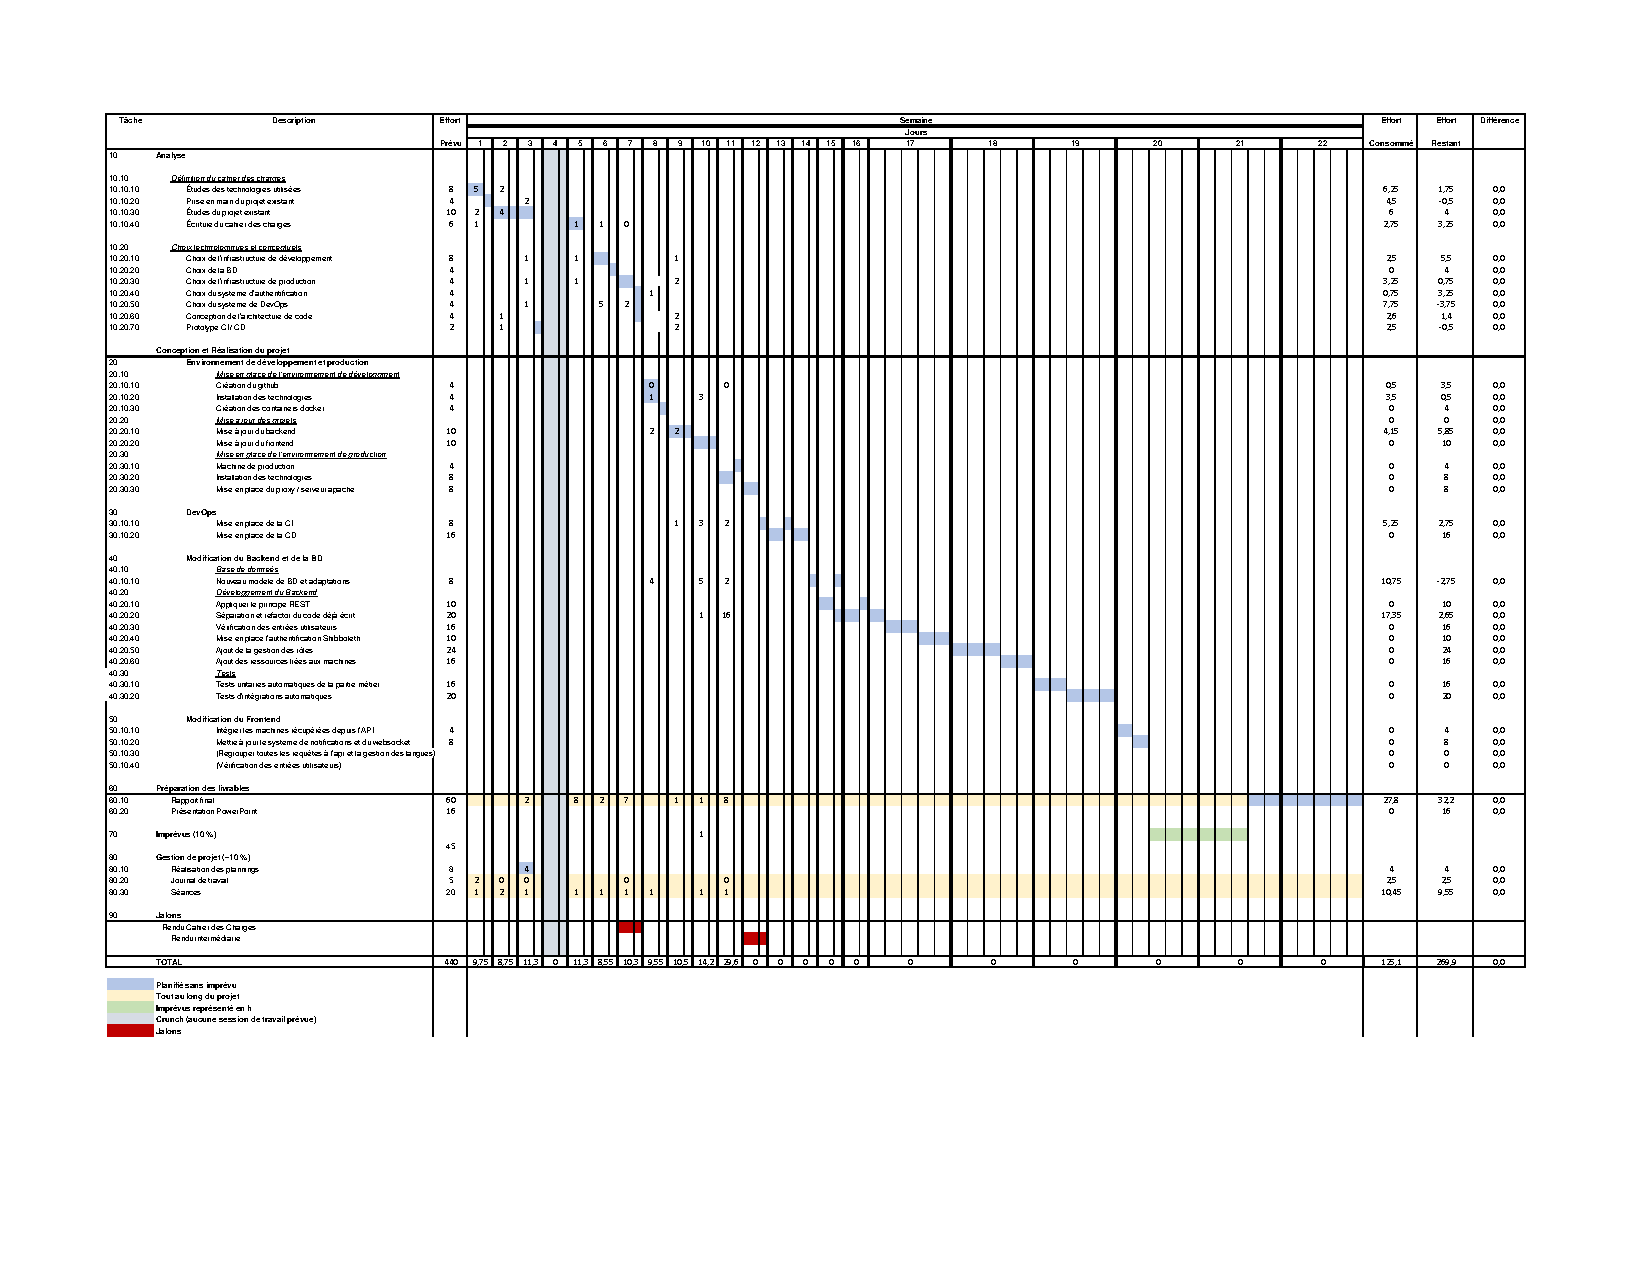
\includepdf{./assets/annexes/planning-v1.pdf}
\end{landscape}

\begin{landscape}
    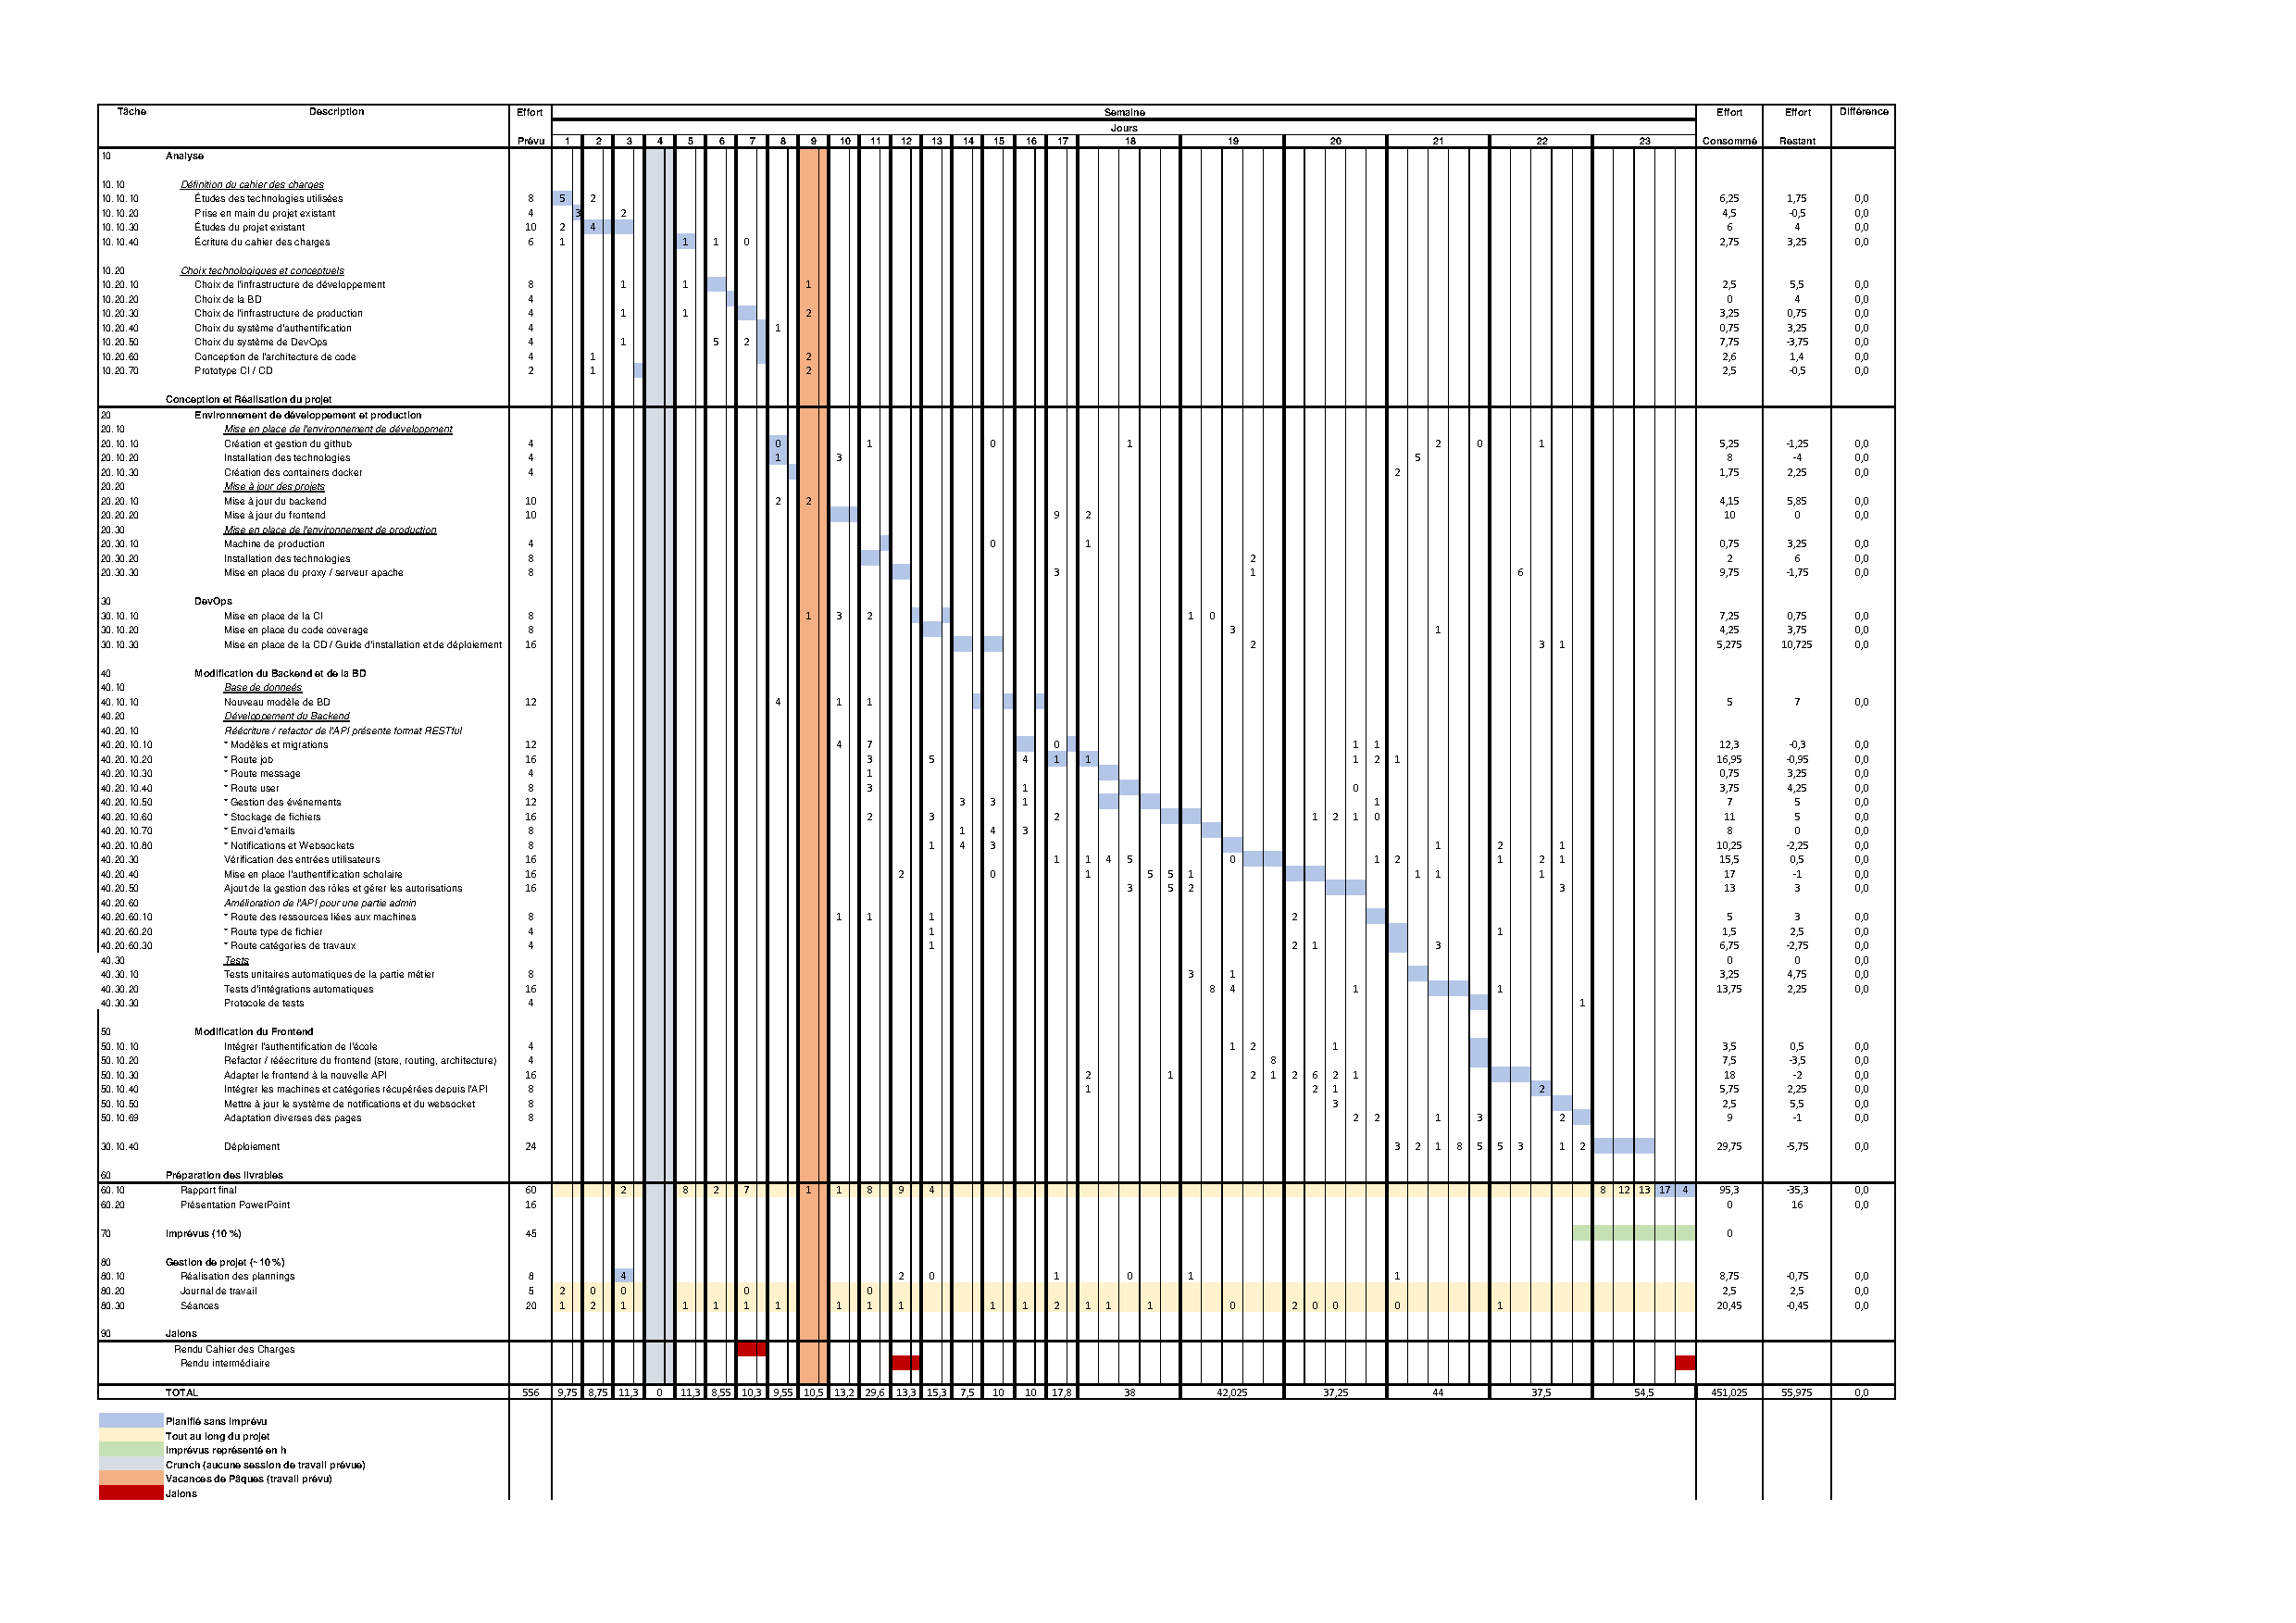
\includepdf{./assets/annexes/planning-v7.pdf}
\end{landscape}

\chapter{Docker}

\section{Introduction à Docker}
Pour pour pouvoir comparer les différentes infrastructures et faire des choix sur ces dernières, il est important d'introduire l'outil \Gls{docker}.\\
\Gls{docker} est un outil permettant de gérer des conteneurs.\\
Qu'est-ce qu'un \Gls{conteneur}? Un \Gls{conteneur} est une sorte de machine virtuelle plus légère ayant pour but d'encapsuler une ou plusieurs applications / outils technologiques ainsi que toutes les dépendances que ces applications exigent pour leur bon fonctionnement.\\
Il ne s'agit donc pas de virtualisation mais de \emph{conteneurisation} ou \emph{containerization} en anglais.
Dans une \emph{conteneurisation}, seul l'\Gls{os} et le software est virtualisé et non le hardware.\\
Nous remarquons bien la différence avec la figure suivante \ref{docker-compare}

\begin{center}
    \begin{figure}[H]
        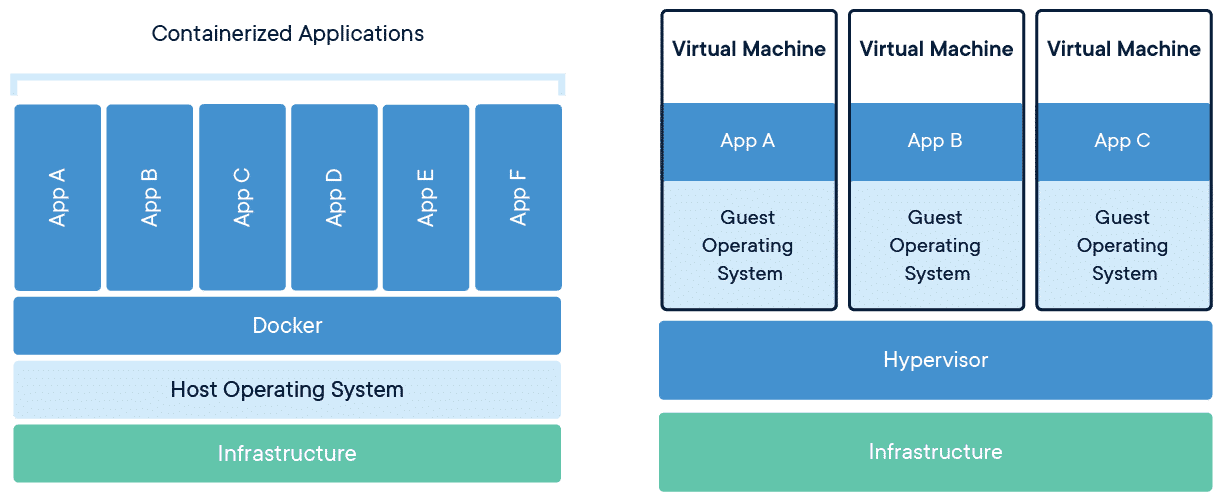
\includegraphics[width=\textwidth]{./assets/figures/docker-containerized-and-vm.png}
        \caption[Comparaison Docker vs VM]{Comparaison entre containeurs Docker et machines virtuelles
            du \href{https://www.docker.com/wp-content/uploads/2021/11/}{site Docker}
            \label{docker-compare}}
    \end{figure}
\end{center}

Les containers sont facilement téléchargeables et transmissibles. Ils sont également relativement facile à mettre en place.\\
Le principe est simple, nous avons une application et une certaine configuration qui fonctionne, nous pouvons facilement l'encapsuler dans un \Gls{conteneur} et le transmettre à nos collègues ou le télécharger sur un autre pc.\\
Un des principals avantages, est le fait que le \Gls{conteneur} ne dépend pas de l'\Gls{os} ou de l'état de la machine sur lequel il va être lancé.\\
Le seul point requis, est de posséder \Gls{docker} sur la machine.\\
Cette solution rend plus flexible et portable l'exécution d'application sur n'importe quelle machine.\\
Voici un schéma démontrant la façon dont \Gls{docker} et des \Gls{conteneur}s \Gls{docker} sont mis en place sur une
machine comme illustré sur la figure \ref{docker-container-app}.

\begin{center}
    \begin{figure}[H]
        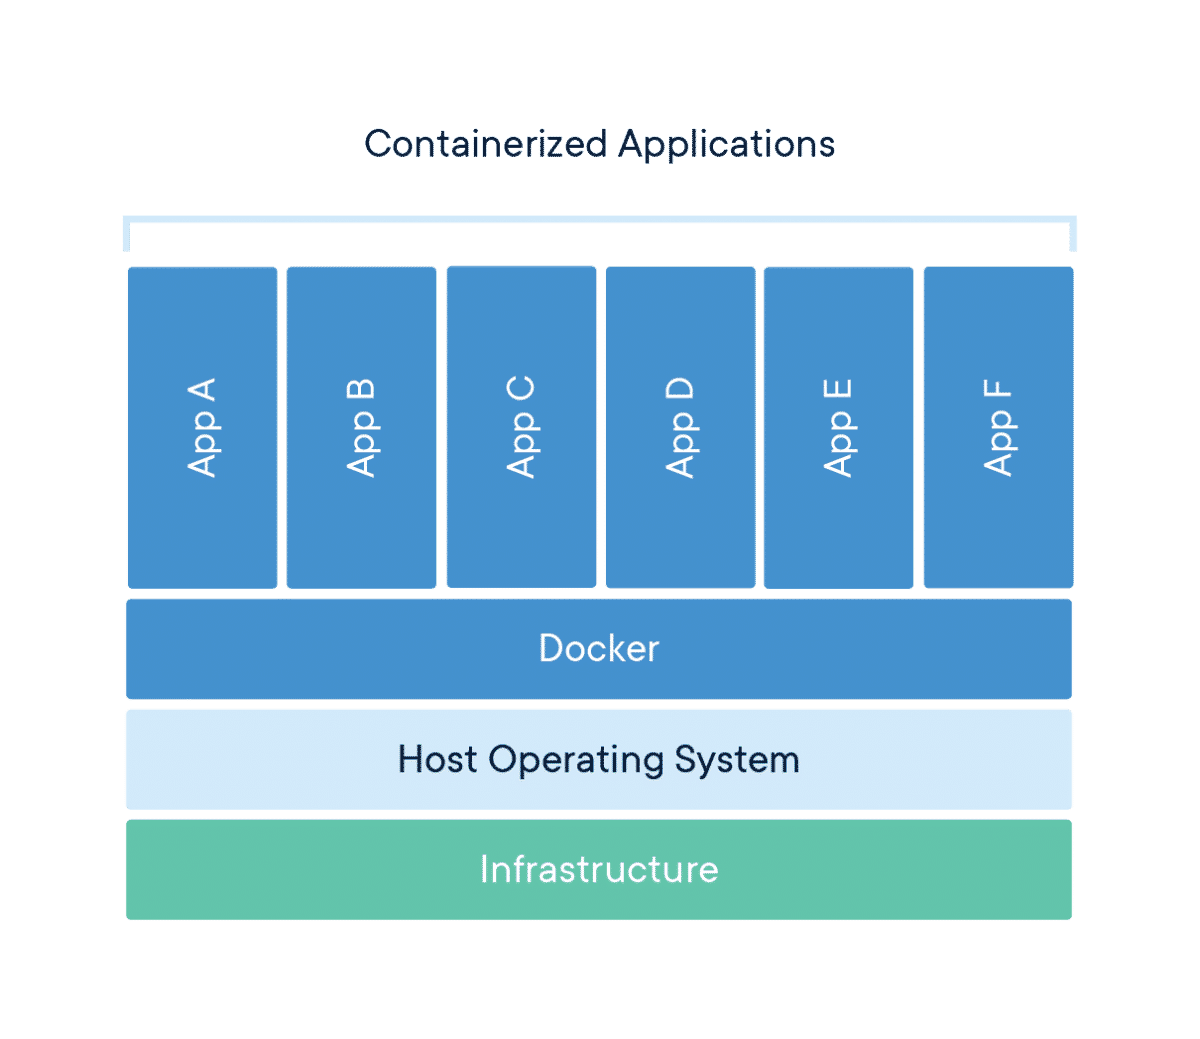
\includegraphics[width=\textwidth]{./assets/figures/container-what-is-container.png}
        \caption[Conteneurisation d'applications]{Conteneurisation d'applications via
            le \href{https://www.docker.com/wp-content/uploads/2021/11/container-what-is-container.png}{site docker}
            \label{docker-container-app}}
    \end{figure}
\end{center}

%https://www.docker.com/resources/what-container/
%https://www.ibm.com/fr-fr/cloud/learn/docker
%https://fr.wikipedia.org/wiki/Docker_(logiciel)
%https://www.youtube.com/watch?v=Gjnup-PuquQ

Voici une liste des avantages généraux de \Gls{docker} comparé à une VM:
\begin{itemize}
    \item + Les \Gls{conteneur}s sont petits comparé au VM \cite{koukia,nick}; %\char{2713}
    \item + Les \Gls{conteneur}s utilisent moins de ressources \cite{koukia};
    \item + Les \Gls{conteneur}s démarrent plus rapidement \cite{koukia};
    \item + Fonctionne bien avec les \Gls{devops} et les \Gls{ci}/\Gls{cd} \cite{koukia,data-flair-pros-cons,data-flair-use-cases};
    \item + Facilite l'extensibilité horizontale \cite{data-flair-use-cases};
    \item + Regroupe les applications et les fichiers système en une seule image standardisée \cite{kane2018docker};
    \item + Permet de tester et livrer l'exact même artefact à tous les systèmes et dans tous les
          environnements \cite{kane2018docker,nick};
    \item + Créer une abstraction autour de l'application sans sacrifier trop de ressources \cite{kane2018docker}.
\end{itemize}

Voici une liste des inconvénients de \Gls{docker} comparé à une VM:
\begin{itemize}
    \item - La sécurité; \cite{koukia}
    \item - L'isolation non complète'; \cite{koukia}
    \item - La gestion du réseau. \cite{koukia}
\end{itemize}

Pour terminer, nous pouvons voir sur la figure \ref{docker-use-cases} une liste des cas d'utilisations de \Gls{docker} \cite{data-flair-use-cases}.

\begin{center}
    \begin{figure}[H]
        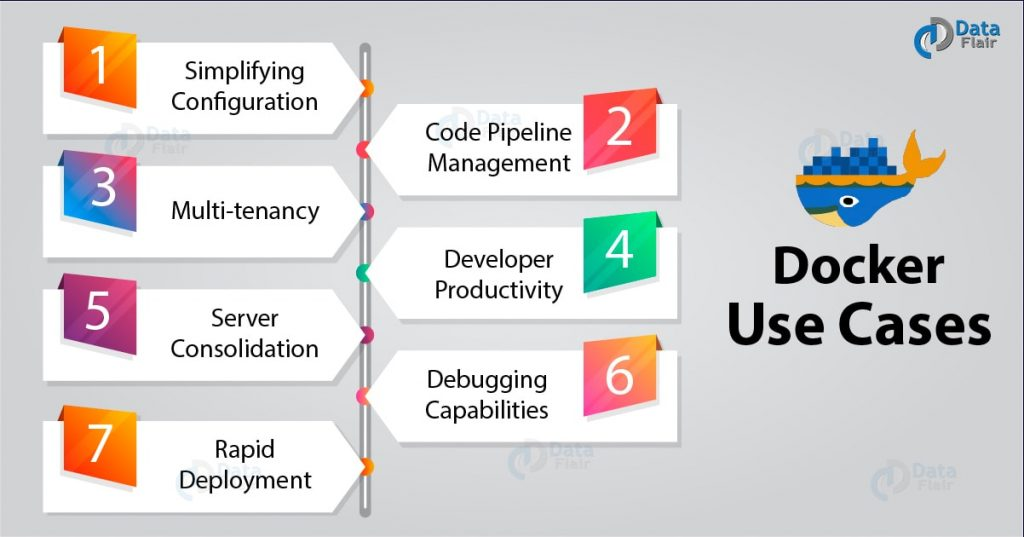
\includegraphics[width=\textwidth]{./assets/figures/docker-use-cases.jpg}
        \caption[Cas d'utilisation de docker]{Cas d'utilisation de docker via \href{https://data-flair.training/blogs/wp-content/uploads/sites/2/2018/10/}{data falir}
            \label{docker-use-cases}}
    \end{figure}
\end{center}

\subsubsection{Docker point de vue sécurité}
En ce qui concerne la sécurité de \Gls{docker}, je ne me suis pas assez plongé dedans pour ressortir une
analyse concrète et fiable mais j'ai trouvé un article \cite{combe} qui en parle et qui pourrait
être une première direction pour approfondir le sujet.

% Packaging software in a way that leverages the skills developers already have. \cite{kane2018docker}
% Bundling application software and required OS filesystems together in a single standar‐dized image format. \cite{kane2018docker}
% Using packaged artifacts to test and deliver the exact same artifact to all systems in all environments. \cite{kane2018docker}
% Abstracting software applications from the hardware without sacrificing resources \cite{kane2018docker}

% quand ne pas utiliser docker: Performance is critical to your application

%virtual machine vs containers:
%https://www.youtube.com/watch?v=cjXI-yxqGTI
%https://www.ibm.com/cloud/learn/containers?utm_medium=OSocial&utm_source=Youtube&utm_content=000023UA&utm_term=10010608&utm_id=YTDescription-101-Containers-vs-VMs-LH-Containers-Guide&cm_mmc=OSocial_Youtube-_-Cloud+and+Data+Platform_SFT+Cloud+Platform+Digital-_-WW_WW-_-YTDescription-101-Containers-vs-VMs-LH-Containers-Guide&cm_mmca1=000023UA&cm_mmca2=10010608
%https://www.ibm.com/cloud/learn/virtual-machines?utm_medium=OSocial&utm_source=Youtube&utm_content=000005UJ&utm_term=10002434&utm_id=YTDescription-101-Containers-vs-VMs-LH-Virtual-Machines-Guide&cm_mmc=OSocial_Youtube-_-Cloud+and+Data+Platform_PLT+Cloud+Platform+F2F-_-WW_WW-_-YTDescription-101-Containers-vs-VMs-LH-Virtual-Machines-Guide&cm_mmca1=000005UJ&cm_mmca2=10002434


\section{Performances de Docker}
\Gls{docker} est outil qui paraît très pratique, mais qu'en est-il de ses performances?
Pour ceci, nous allons retracer quelques évalutations réalisées lors d'une étude de IBM. Nous allons parcourir ces évalutations via des graphiques, tiré de l'étude, résumants bien les résultats.
Commençant par la latence que peut apporter \Gls{docker} indiquée sur la figure \ref{network-latency}.

\begin{center}
    \begin{figure}[H]
        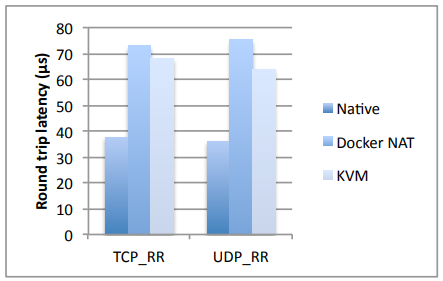
\includegraphics[width=\textwidth]{./assets/figures/docker-perf-latency.png}
        \caption[Docker latence aller-retour du réseau]{Latence aller-retour du réseau (µs) \cite{rad2017introduction} \label{network-latency}}
    \end{figure}
\end{center}

Nous constatons que la latence double, mais nous parlons ici de microsecondes, et de 30 microsecondes supplémentaires, ce qui est en soit assez peu pour de petite infrastructure.

En ce qui concerne le transfert de grosses quantité de données via \gls{tcp}, \Gls{docker} parvient à se
rapprocher des performances d'une machine native, elles n'utilisent donc pas beaucoup plus de cycles
comme illustré dans la figure \ref{tcp-transfer-latency}.

\begin{center}
    \begin{figure}[H]
        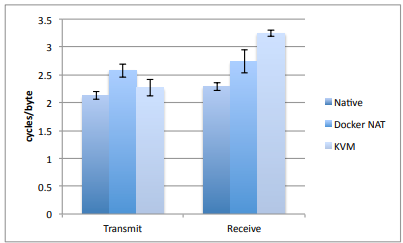
\includegraphics[width=\textwidth]{./assets/figures/docker-perf-transfer-efficiancy.png}
        \caption[Docker efficacité du transfert de masse]{Efficacité du transfert de masse TCP (cycles CPU/octet) \cite{rad2017introduction} \label{tcp-transfer-latency}}
    \end{figure}
\end{center}

Au niveau des écritures, nous remarquons grâce aux deux graphiques suivants que les performances valent
celles d'un système natif comme le montre les figures \ref{sequential-io} et \ref{random-io}

\begin{center}
    \begin{figure}[H]
        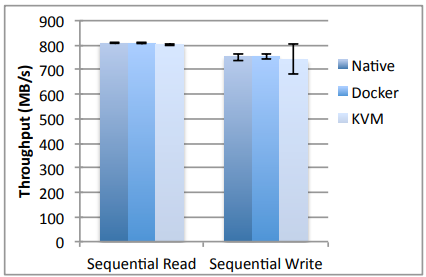
\includegraphics[width=\textwidth]{./assets/figures/docker-perf-sequential-io.png}
        \caption[Docker débit d'I/O séquentielles]{Débit d'Entrée/Sortie séquentielles (Mo/s) \cite{rad2017introduction} \label{sequential-io}}
    \end{figure}
\end{center}

\begin{center}
    \begin{figure}[H]
        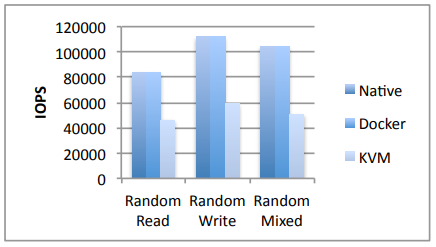
\includegraphics[width=\textwidth]{./assets/figures/docker-perf-random-io.png}
        \caption[Débit d'I/O aléatoires]{Débit d'Entrée/Sortie aléatoires (IOPS) \cite{rad2017introduction} \label{random-io}}
    \end{figure}
\end{center}

Nous pouvons également observer sur la figure \ref{docker-perf-mysql} des performances sur le \Gls{sgbd} \Gls{mysql}
que nous utilisons pour le projet.

\begin{center}
    \begin{figure}[H]
        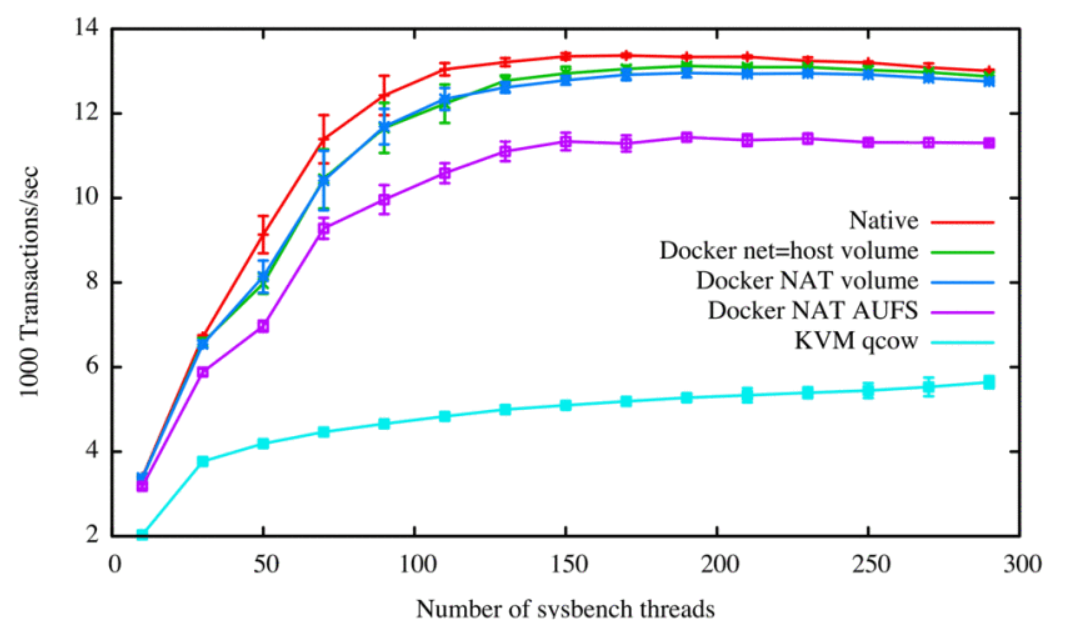
\includegraphics[width=\textwidth]{./assets/figures/docker-perf-mysql.png}
        \caption[Comparaison des perf. Docker sur MySQ]{Comparaison des performances de Docker avec des transactions sur MySQL \cite{felter} \label{docker-perf-mysql}}
    \end{figure}
\end{center}

Beaucoup d'autres informations ressortent dans un article étudiant les performances de \Gls{docker} pour
des applications demandant une grande performance. \cite{chung}
Un point intéressant, qui me paraît important, est celui de la gestion de la mémoire vive qu'utilise
\Gls{docker}, illustré sur la figure \ref{docker-perf-ram}.\\
Nous voyons clairement que \Gls{docker} n'est pas pas plus gourmand qu'une machine native et c'est un bon point.

\begin{center}
    \begin{figure}
        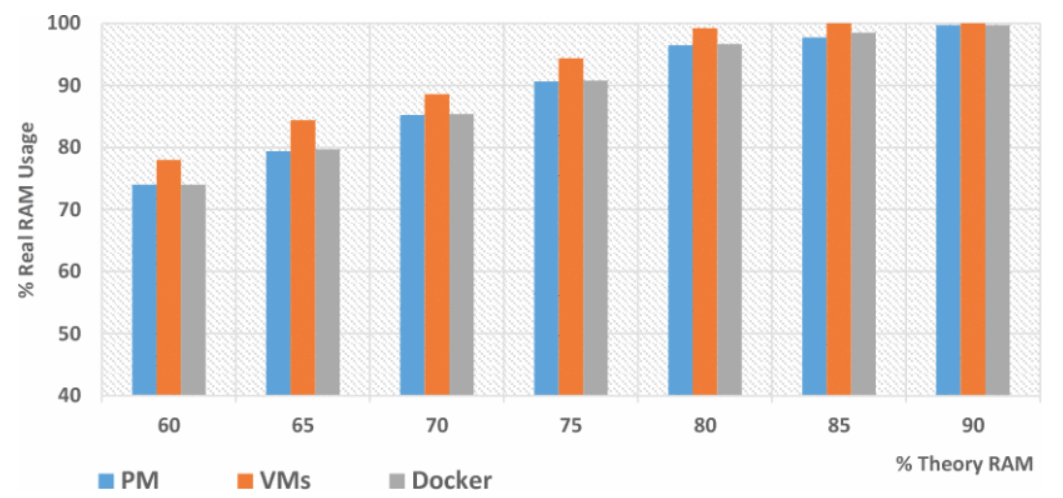
\includegraphics[width=\textwidth]{./assets/figures/docker-perf-ram.png}
        \caption[Comparaison des perf. Docker sur la RAM]{Comparaison des performances de Docker au
            niveau de l'utilisation de la mémoire vive \cite{chung} \label{docker-perf-ram}}
    \end{figure}
\end{center}

%docker en prod perf:
%https://stackoverflow.com/questions/21691540/how-to-optimize-performance-for-a-docker-container/21707838#21707838
%https://stackoverflow.com/questions/21889053/what-is-the-runtime-performance-cost-of-a-docker-container
%https://dominoweb.draco.res.ibm.com/reports/rc25482.pdf
%https://www.freecodecamp.org/news/7-cases-when-not-to-use-docker/

\section{Et Kubernetes?}
Pourquoi utiliserions-nous forcément \Gls{docker} sans avoir réfléchi à la possibilité de \Gls{kubernetes}?
Pour commencer, comme indiquer sur le site officiel:
"\Gls{kubernetes} est un système open-source permettant d'automatiser le déploiement, la mise à l'échelle et la gestion des applications conteneurisées".\\
\Gls{kubernetes} n'est donc pas vraiment une alternative à \Gls{docker}, mais peut être plutôt utiliser comme complément à ce dernier.\\
Comme la partie principale de \Gls{kubernetes} est de gérer les applications conteneurisées et de simplifier le load balancing, par exemple, il n'est pas forcément utile pour nous d'approfondir les recherches sur le sujet.\\
En effet, La charge attendu par l'application déployée ne devrait pas dépasser les 100 utilisateurs simultanés. La question du load-balancing est donc écartée, tout comme la mise en place d'un cluster \Gls{kubernetes}.

% comment mettre en place -> voir avec monsieur Graf / regarder avec des profs
% si question pointu, peuvent être transférer à m. chevallier

%https://kubernetes.io/
%https://www.youtube.com/watch?v=PziYflu8cB8
%docker vs k8s, IBM: https://www.youtube.com/watch?v=2vMEQ5zs1ko
%https://www.ibm.com/cloud/learn/kubernetes?cm_mmc=OSocial_Youtube-_-Hybrid+Cloud_Cloud+Platform+Digital-_-WW_WW-_-KubevsDockerYTDescription&cm_mmca1=000023UA&cm_mmca2=10010608#toc-what-is-ku-nVcfWlWE

%https://stackshare.io/: outil très utile pour faire des comparaisons de technologies

\section{Autres solutions de conteneurs}
Une question se pose, pourquoi utiliserions-nous forcément \Gls{docker} alors que d'autres solutions existent?
Pour commencer, voici une liste non exhaustive des solutions alternatives à \Gls{docker}:
\begin{itemize}
    \item \href{https://fr.wikipedia.org/wiki/BSD_Jail}{BSD Jails};
    \item \href{https://linuxcontainers.org/lxd/}{LXD};
    \item \href{https://linuxcontainers.org/lxc/introduction/}{LXC};
    \item \href{https://docs.oracle.com/cd/E18440_01/doc.111/e18415/chapter_zones.htm#OPCUG426}{Solaris Zones};
    \item \href{https://www.redhat.com/en/topics/containers/what-is-rkt}{RKT}.
\end{itemize}

Le principal problème de ces solutions est le manque de popularité comme nous pouvons le remarquer sur la
figure \ref{containers-trends} représentant les recherches concernant les différents sujets via l'outil \href{https://trends.google.fr/trends}{Google trends}.\\
Le fait de ne pas être populaire est un gros désavantage pour ces solutions car très peu d'informations, de tutoriels et de documentations sont disponibles sur internet.\\
Ce simple fait suffit à orienté le choix de la solution de \Gls{conteneur} sur \Gls{docker}.\\
N'ayant également pas le temps d'analyser chaque solution en profondeur dans ce travail, cela conforte mon choix.

\begin{center}
    \begin{figure}[H]
        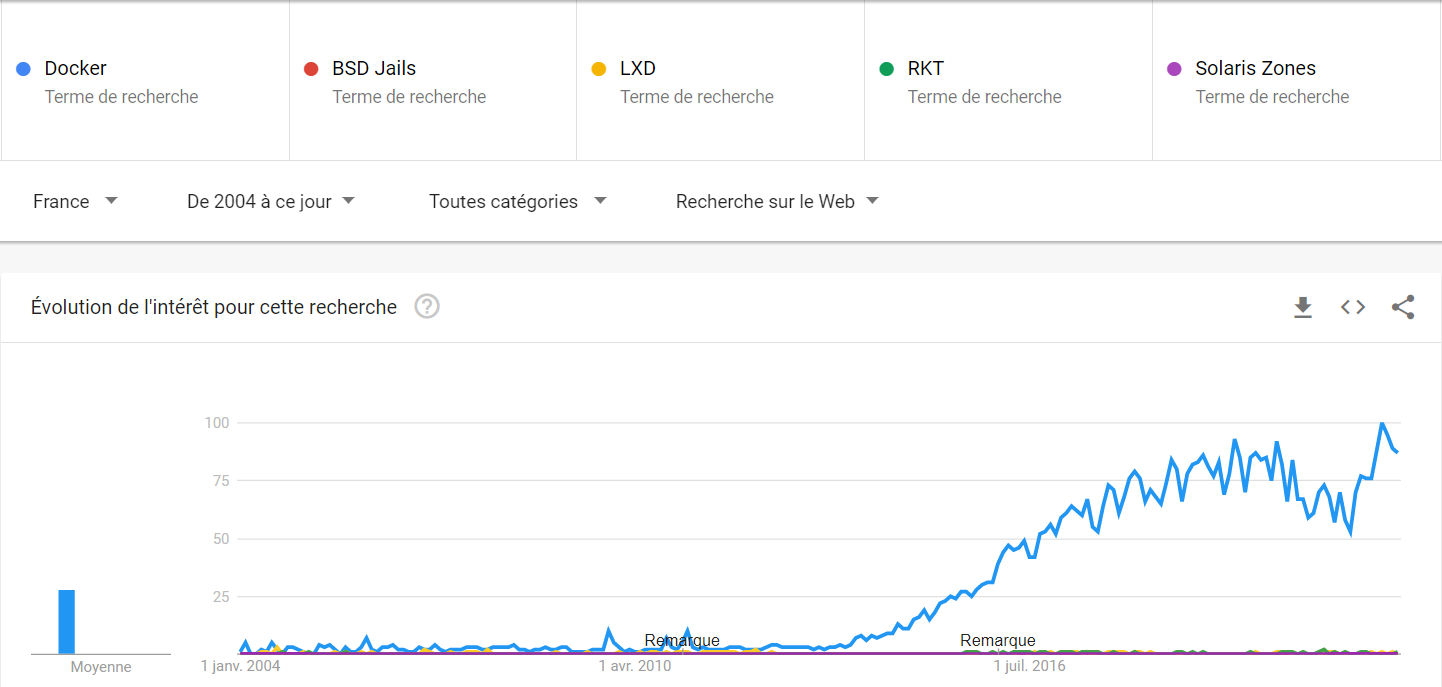
\includegraphics[width=\textwidth]{./assets/figures/google-trend-containers-2022.png}
        \caption[Tendances solutions de conteneurs]{Tendances sur les différentes solutions de conteneurs depuis 2004 \label{containers-trends}}
    \end{figure}
\end{center}

\chapter{Guides}

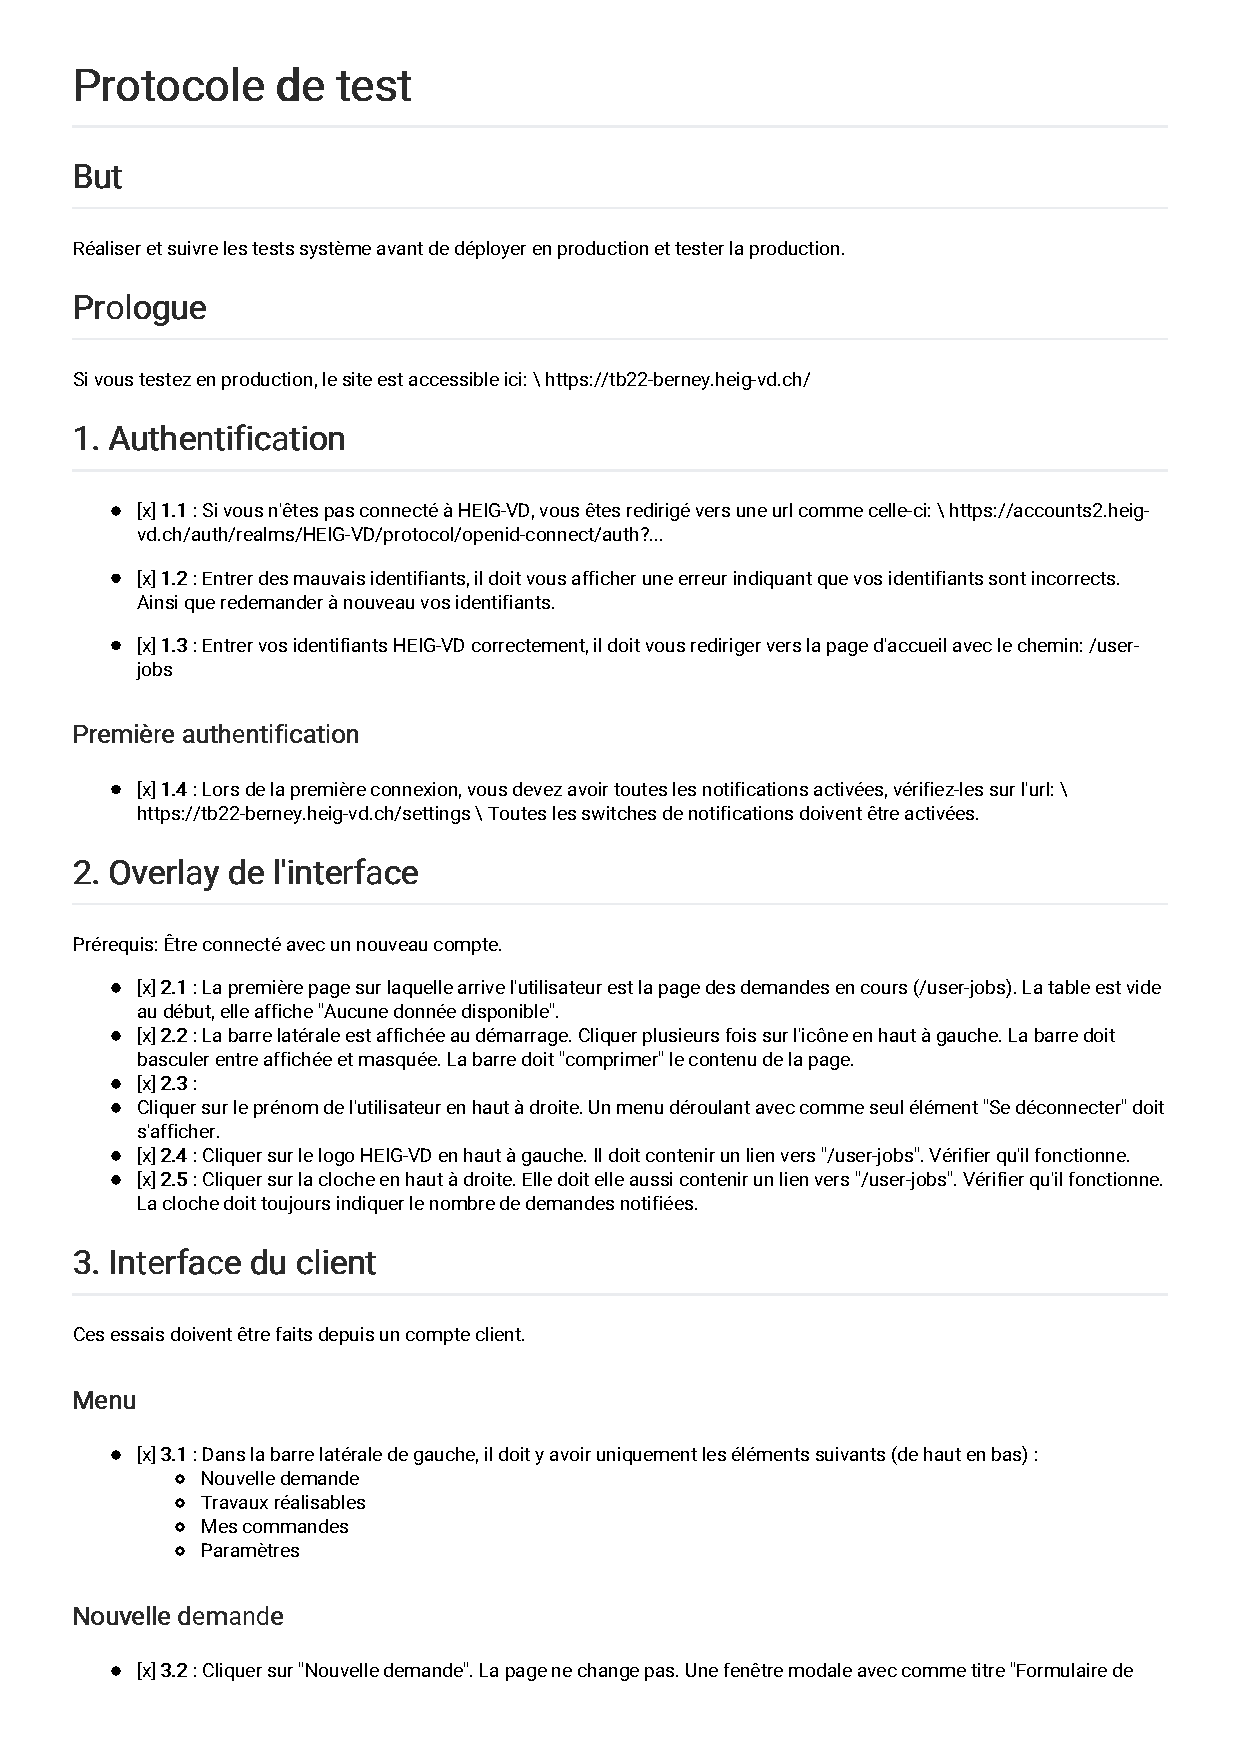
\includepdf[pages={1-}]{./assets/annexes/test-protocole.pdf}

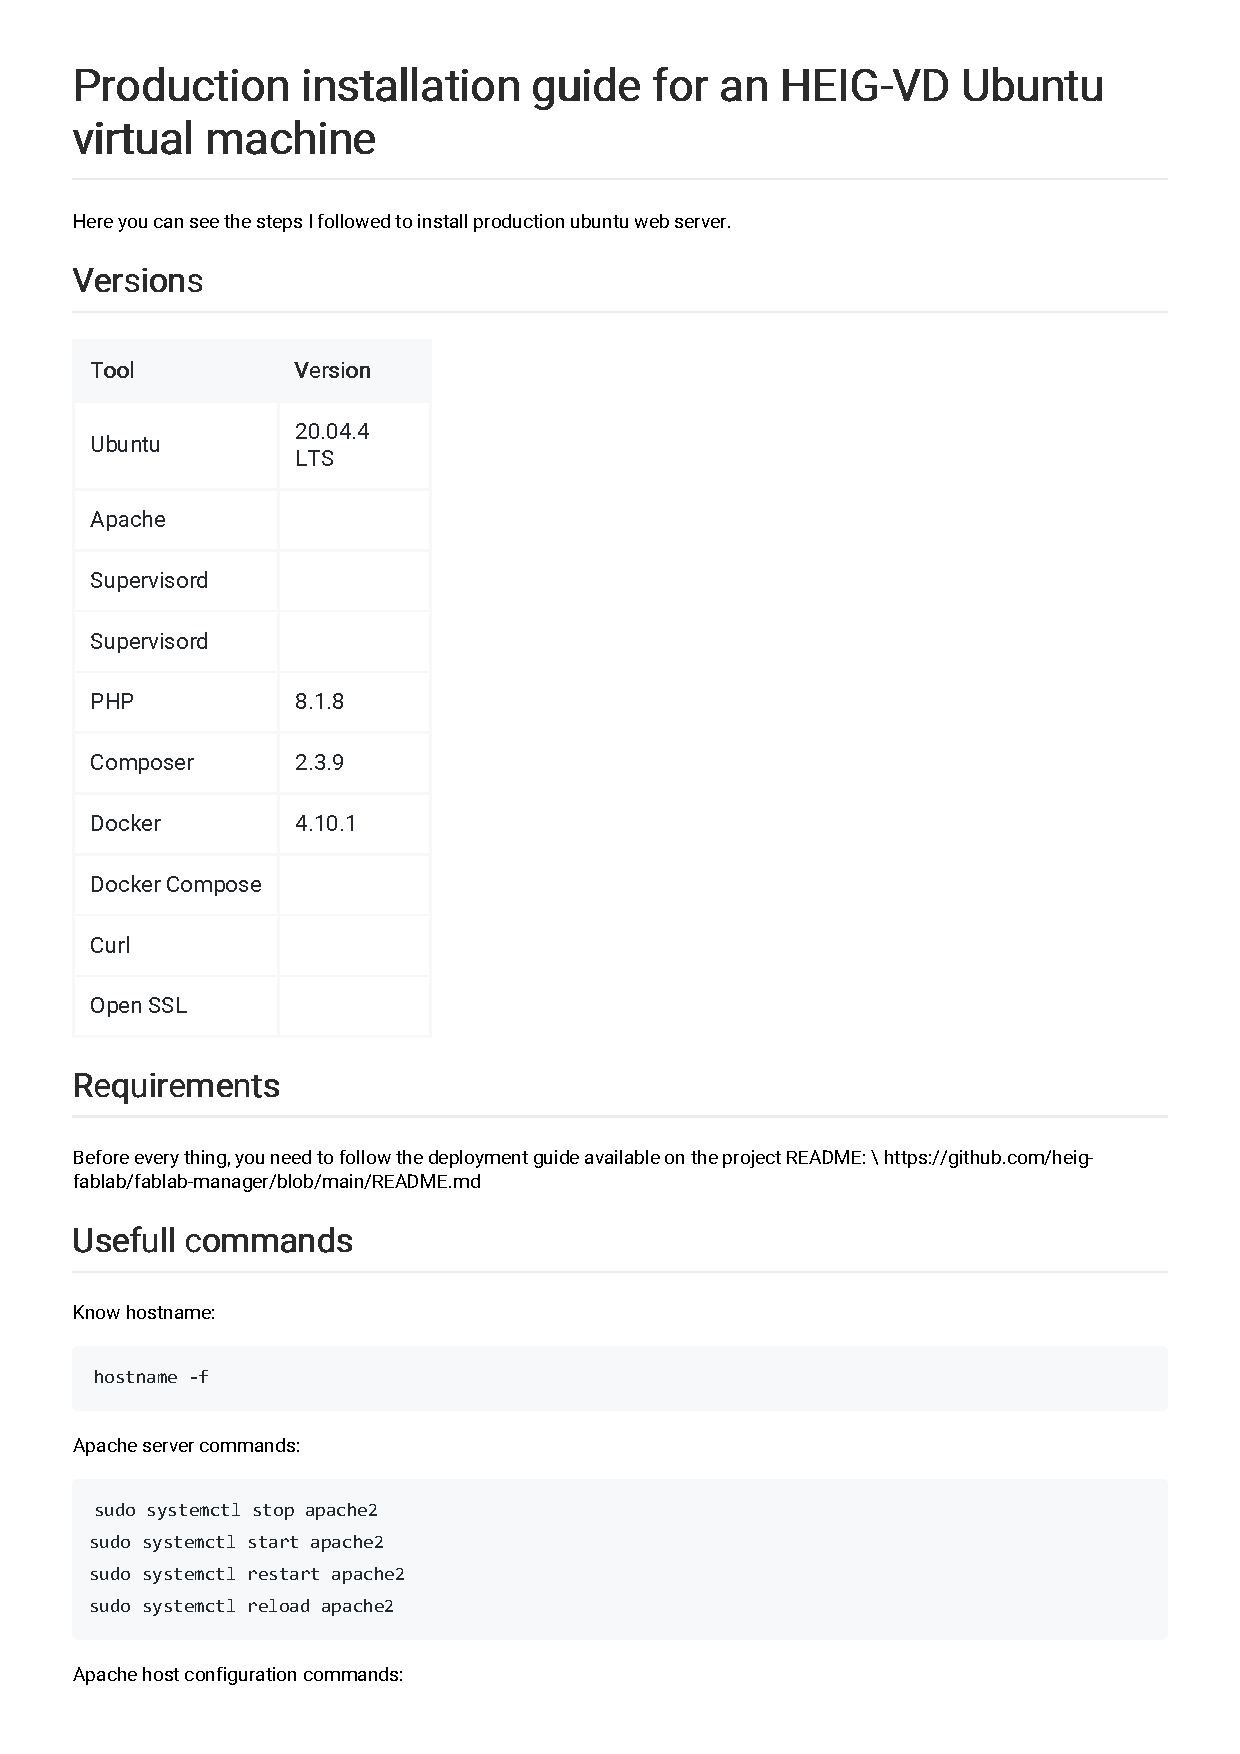
\includepdf[pages={1-}]{./assets/annexes/prod-install-guide.pdf}

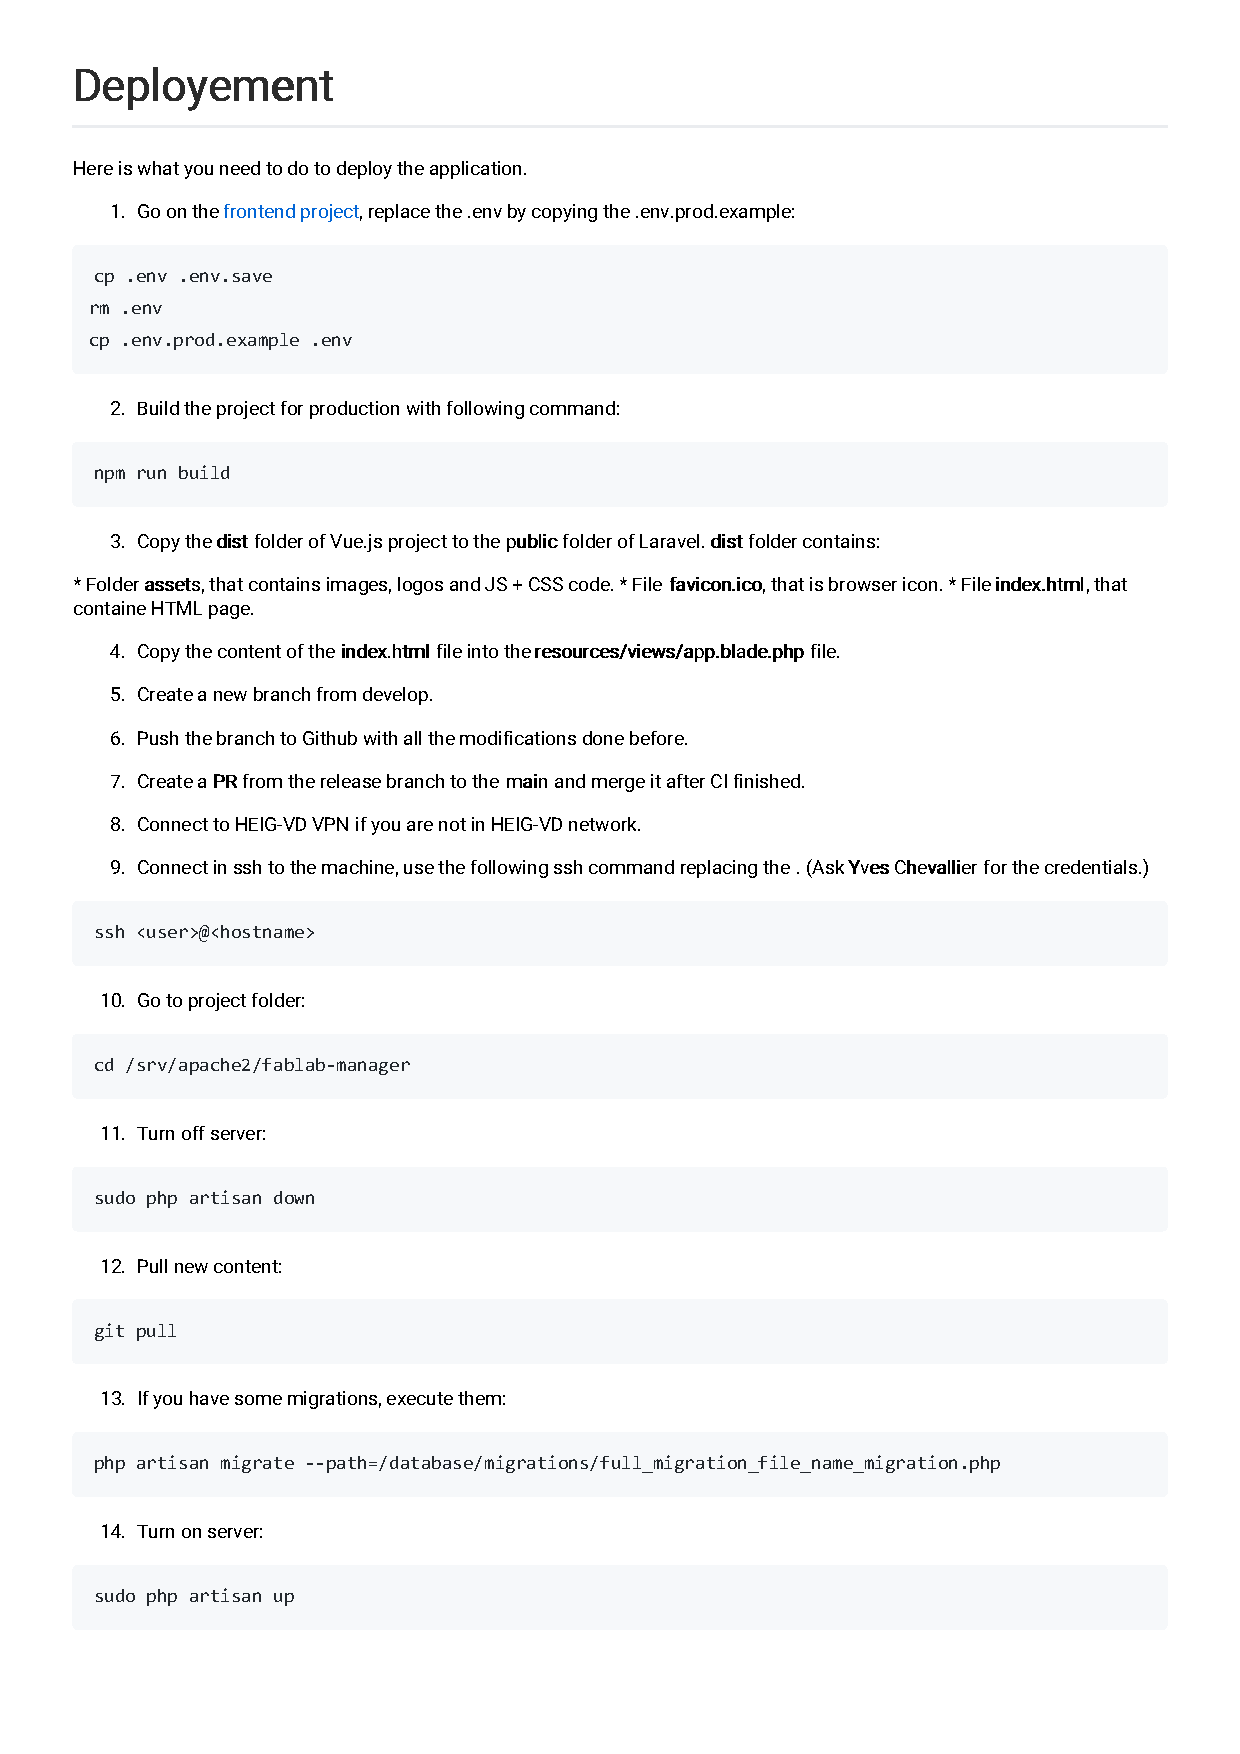
\includepdf[pages={1-}]{./assets/annexes/release.pdf}

\chapter{Code}

\section{Docker-compose}

\begin{listing}[h]
    \inputminted{yaml}{assets/code/docker-compose-mysql.yml}
    \caption{\emph{Docker-compose} pour la base de données \emph{MySQL} \label{docker-compose-mysql}}
\end{listing}

\section{Fichier env}

\begin{listing}[h]
    \inputminted{text}{assets/code/.env.backend.prod}
    \caption{Fichier \emph{.env} du Backend de la production \label{env-backend-prod}}
\end{listing}

\begin{listing}[h]
    \inputminted{text}{assets/code/.env.backend.dev}
    \caption{Fichier \emph{.env} du Backend du développement \label{env-backend-dev}}
\end{listing}

\begin{listing}[h]
    \inputminted{text}{assets/code/.env.frontend.prod}
    \caption{Fichier \emph{.env} du Frontend de la production \label{env-frontend-prod}}
\end{listing}

\begin{listing}[h]
    \inputminted{text}{assets/code/.env.frontend.dev}
    \caption{Fichier \emph{.env} du Frontend du développement \label{env-frontend-dev}}
\end{listing}

\section{Migrations}

\begin{listing}[h]
    \inputminted{php}{assets/code/12_create_file_types_table.php}
    \caption{Migration de la table \emph{file\_types} \label{migrations-file-types}}
\end{listing}

\begin{listing}[h]
    \inputminted{php}{assets/code/13_create_roles_table.php}
    \caption{Migration de la table \emph{roles} \label{migrations-roles}}
\end{listing}

\begin{listing}[h]
    \inputminted{php}{assets/code/14_create_users_table.php}
    \caption{Migration de la table \emph{users} \label{migrations-users}}
\end{listing}

\begin{listing}[h]
    \inputminted{php}{assets/code/15_create_job_categories_table.php}
    \caption{Migration de la table \emph{job\_categories} \label{migrations-job-categories}}
\end{listing}

\begin{listing}[h]
    \inputminted{php}{assets/code/17_create_events_table.php}
    \caption{Migration de la table \emph{events} \label{migrations-events}}
\end{listing}

\begin{listing}[h]
    \inputminted{php}{assets/code/18_create_files_table.php}
    \caption{Migration de la table \emph{files} \label{migrations-files}}
\end{listing}

\begin{listing}[h]
    \inputminted{php}{assets/code/19_create_messages_table.php}
    \caption{Migration de la table \emph{messages} \label{migrations-messages}}
\end{listing}

\begin{listing}[h]
    \inputminted{php}{assets/code/21_create_file_type_job_category_table.php}
    \caption{Migration de la table \emph{file\_type\_job\_category} \label{migrations-file-type-job-category}}
\end{listing}

\begin{listing}[h]
    \inputminted{php}{assets/code/22_create_role_user_table.php}
    \caption{Migration de la table \emph{role\_user} \label{migrations-role-user}}
\end{listing}

\section{Keycloak}

\begin{listing}[h]
    \inputminted{php}{assets/code/KeycloakGuard1.php}
    \caption{KeycloakGuard 1 \label{keycloak-guard1}}
\end{listing}

\begin{listing}[h]
    \inputminted{php}{assets/code/KeycloakGuard2.php}
    \caption{KeycloakGuard 2 \label{keycloak-guard2}}
\end{listing}

\begin{listing}[h]
    \inputminted{php}{assets/code/KeycloakGuard3.php}
    \caption{KeycloakGuard 3 \label{keycloak-guard3}}
\end{listing}

\begin{listing}[h]
    \inputminted{php}{assets/code/Token.php}
    \caption{Token pour Keycloak \label{keycloak-token}}
\end{listing}

\let\cleardoublepage\clearpage
\backmatter

\label{glossaire}
\printnoidxglossary
\printbibliography
\label{index}
\printindex

\end{document}
